%% GABARIT POUR MÉMOIRE STANDARD
%%
%% Consulter la documentation de la classe ulthese pour une
%% description détaillée de la classe, de ce gabarit et des options
%% disponibles.
%%
%% [Ne pas hésiter à supprimer les commentaires après les avoir lus.]
%%
%% Déclaration de la classe avec le type de grade
%%   [l'un de MATDR, MArch, MA, LLM, MErg, MMus, MPht, MSc, MScGeogr,
%%    MServSoc, MPsEd]
%% et les langues les plus courantes. Le français sera la langue par
%% défaut du document.
\documentclass[MSc,english,french]{ulthese}
  %% Encodage utilisé pour les caractères accentués dans les fichiers
  %% source du document. Les gabarits sont encodés en UTF-8. Inutile
  %% avec XeLaTeX, qui gère Unicode nativement.
  \ifxetex\else \usepackage[utf8]{inputenc} \fi

  %% Charger ici les autres paquetages nécessaires pour le document.
  %% Quelques exemples; décommenter au besoin.
  \usepackage{amsmath}       % recommandé pour les mathématiques
  \usepackage{icomma}        % gestion de la virgule dans les nombres
  \usepackage{amssymb}
  %% Utilisation d'une autre police de caractères pour le document.
  %% - Sous LaTeX
  \usepackage{tgpagella}      % texte et mathématiques en Palatino
  % \usepackage{mathptmx}      % texte et mathématiques en Times
  %% - Sous XeLaTeX
  %\setmainfont{TeX Gyre Pagella}      % texte en Pagella (Palatino)
  %\setmathfont{TeX Gyre Pagella Math} % mathématiques en Pagella (Palatino)
  %\setmainfont{TeX Gyre Termes}       % texte en Termes (Times)
  %\setmathfont{TeX Gyre Termes Math}  % mathématiques en Termes (Times)

  %% Options de mise en forme du mode français de babel. Consulter la
  %% documentation du paquetage babel pour les options disponibles.
  %% Désactiver (effacer ou mettre en commentaire) si l'option
  %% 'nobabel' est spécifiée au chargement de la classe.
  \frenchbsetup{%
    StandardItemizeEnv=true,       % format standard des listes
    ThinSpaceInFrenchNumbers=true, % espace fine dans les nombres
    og=«, fg=»                     % caractères « et » sont les guillemets
  }

  %% Style de la bibliographie.  

  \titre{Approches de bandits pour la\\ génération automatique de résumés de textes}
  \auteur{Mathieu Godbout}
  \programme{Maîtrise en informatique}
  \codirection{Luc Lamontagne, codirecteur de recherche \\
              Audrey Durand, codirectrice de recherche}


\usepackage{tikz}
\usepackage{ctable}
\usepackage{graphicx}
\usetikzlibrary{intersections}
\usetikzlibrary{external}
\usetikzlibrary{shapes.misc, positioning, fit, arrows.meta, arrows, shapes, backgrounds, calc}
\tikzexternalize[prefix=figures/]

\usepackage{pgfplots}
\usepackage{pgfplotstable}
\usepgfplotslibrary{colorbrewer}
\usepgfplotslibrary{fillbetween}
\pgfplotsset{compat=1.16, colormap/Blues, every axis/.append style={label style={font=\large}, tick label style={font=\large}}}

\usepackage{mathtools}
\DeclarePairedDelimiter{\ceil}{\lceil}{\rceil}
\DeclareMathOperator*{\argmax}{arg\,max}
\DeclareMathOperator*{\argmin}{arg\,min}


\usepackage[mathscr]{euscript}
\let\euscr\mathscr \let\mathscr\relax
\usepackage[scr]{rsfso}

\usepackage{xcolor}
\newcommand\todo[1]{\textcolor{red}{TODO: #1}}
\newcommand\question[1]{\textcolor{blue}{Question: #1}}
\newcommand\commentaire[1]{\textcolor{violet}{Commentaire: #1}}
\newcommand\ngrams{\textit{n}-grammes }

\usepackage{mathtools}

\DisemulatePackage{setspace}
\usepackage{setspace}

\addto\captionsfrench{\def\tablename{Tableau}}

  % French version of algorithmic
  \usepackage[noend]{algpseudocode}
  \usepackage{algorithm}
  \algnewcommand\AND{\textbf{et} }
	\renewcommand{\listalgorithmname}{Liste des algorithmes}
	\floatname{algorithm}{Algorithme}
	\renewcommand{\algorithmicreturn}{\textbf{retourner}}
	\renewcommand{\algorithmicprocedure}{\textbf{procédure}}
	\renewcommand{\algorithmicrequire}{\textbf{Entrée:}}
	\renewcommand{\algorithmicensure}{\textbf{Sortie:}}
	\renewcommand{\algorithmicend}{\textbf{fin}}
	\renewcommand{\algorithmicif}{\textbf{si}}
	\renewcommand{\algorithmicthen}{\textbf{alors}}
	\renewcommand{\algorithmicelse}{\textbf{sinon}}
	\renewcommand{\algorithmicfor}{\textbf{pour}}
	\renewcommand{\algorithmicforall}{\textbf{pour tout}}
	\renewcommand{\algorithmicdo}{\textbf{faire}}
	\renewcommand{\algorithmicwhile}{\textbf{tant que}}
	\newcommand{\algorithmicelsif}{\algorithmicelse\ \algorithmicif}
	\newcommand{\algorithmicendif}{\algorithmicend\ \algorithmicif}
	\newcommand{\algorithmicendfor}{\algorithmicend\ \algorithmicfor}

\begin{document}

\frontmatter                    % pages liminaires

\frontispice                    % production de la page frontispice

\chapter*{Résumé}               % ne pas numéroter
\label{chap:resume}             % étiquette pour renvois
\phantomsection\addcontentsline{toc}{chapter}{\nameref{chap:resume}} % inclure dans TdM

\begin{otherlanguage*}{french}
  <Texte du résumé en français. Obligatoire.>
\end{otherlanguage*}
                % résumé français
\chapter*{Abstract}             % ne pas numéroter
\label{chap:abstract}           % étiquette pour renvois
\phantomsection\addcontentsline{toc}{chapter}{\nameref{chap:abstract}} % inclure dans TdM

\begin{otherlanguage*}{english}
This thesis discusses the use of bandit methods to solve 
the problem of training extractive abstract generation models.
The extractive models, which build summaries by selecting sentences from an 
original document, are difficult to train because the target summary of a document is usually not built in an extractive way.
It is for this purpose that we propose to see the production of extractive summaries
as different bandit problems, for which there exist algorithms that can be leveraged for training summarization models.

In this paper, BanditSum is first presented, an approach drawn from 
the literature that sees the generation of the summaries 
of a set of documents as a contextual bandit problem.
Next, we introduce CombiSum, a new algorithm 
which formulates the generation of the summary of a 
single document as a combinatorial bandit.
By exploiting the combinatorial formulation,
CombiSum manages to incorporate the notion of the extractive potential 
of each sentence of a document in its training.
Finally, we propose LinCombiSum, the linear variant of CombiSum 
which exploits the similarities between sentences in a document 
and uses the linear combinatorial bandit formulation instead.
 
\end{otherlanguage*}
              % résumé anglais
\cleardoublepage

\maxtocdepth{subsection}
\tableofcontents                % production de la TdM
\cleardoublepage

\listoftables                   % production de la liste des tableaux
\cleardoublepage

\listoffigures                  % production de la liste des figures
\cleardoublepage

\listofalgorithms
\cleardoublepage

\dedicace{À Samantha.}
\cleardoublepage

\epigraphe{"<Texte de l'épigraphe>"}{<Source ou auteur>}
\cleardoublepage

\chapter*{Remerciements}        % ne pas numéroter
\label{chap:remerciements}      % étiquette pour renvois
\phantomsection\addcontentsline{toc}{chapter}{\nameref{chap:remerciements}} % inclure dans TdM

Je tiens à remercier mon directeur de recherche, Luc Lamontagne,
pour ses précieux conseils tout au long de mon parcours à la maîtrise.
Sa bienveillance et sa franchise m'auront permis de progresser non 
seulement en tant que chercheur, mais aussi en tant que personne.
Un merci tout particulier à Audrey Durand, ma co-directrice, pour m'avoir initié 
au passionnant domaine des bandits et de l'apprentissage par renforcement.
À travers nos interactions, j'ai découvert tout le plaisir 
qui se cache derrière le processus scientifique bien fait et je suis
impatient de continuer notre collaboration.
Par leurs efforts conjoints, Luc et Audrey m'ont permis de me 
dépasser et de bâtir mon propre bagage scientifique.

Je ne peux passer sous le silence l'incroyable communauté de recherche 
du Groupe de Recherche en Apprentissage Automatique 
de l'université Laval (GRAAL) dans laquelle j'ai eu la chance de compléter 
ma maîtrise.
Tantôt collègues de travail, tantôt partenaires de célébrations, les 
personnes que j'ai rencontrées au GRAAL ont grandement contribué 
à faire de ma maîtrise une période de ma vie que je chérirai toujours.
Merci à David, Jean-Thomas, Nicolas, Jean-Samuel, Frédérik, Gaël
et tous les autres.

Un merci spécial va aussi à mes parents, Martine et Alain, qui, avec leur éternelle confiance en 
mes capacités et leur dévouement à mon épanouissement ont rendu possible
mon cheminement scolaire et personnel.
Je conserve le dernier de mes remerciements pour Samantha, sans qui je ne serais pas 
l'ombre de la personne que je suis aujourd'hui. 
Partenaire de mes joies comme de mes peines, elle a toujours su faire ressortir 
la meilleure version de moi-même.
Par son écoute, ses questions intéressées et son soutien incomparable,
elle a certainement participé à l'écriture de ce mémoire dans une bien plus grande
proportion qu'elle ne peut l'imaginer.

Je remercie aussi le Conseil de Recherches en Sciences Naturelles et en Génie du Canada
(CRSNG), le Fonds de recherche du Québec — Nature et Technologies (FRQ-NT)
et Intact~Corporation~financière pour leur soutien financier ayant permis l'élaboration de ce document.         % remerciements

\mainmatter                     % corps du document

\chapter{Introduction}
\label{chap:introduction}

Lors d'une entrevue en 2018, le président de la multinationale Siemens 
mentionnait que\footnote{Traduction libre.} "Les données sont le nouveau pétrole, ou or,
du 21ème siècle - la matière première sur laquelle nos économies,
sociétés et démocraties sont de plus en plus bâties."
Son affirmation, partagée par bon nombre d'experts dans le domaine de la
technologie, décrit ce que l'on appelle communément l'ère du \textit{Big Data}.
Cette appellation vise à décrire la quantité immense de données maintenant 
générées et collectées par le traffic internet ou encore les appareils de 
l'Internet des ObjeTs (IoT), pour n'en nommer que quelques-uns.

Dans la panoplie de données à disposition se trouvent les données textuelles, 
issues par exemple d'interactions sur des réseaux sociaux ou encore de documents 
numériques.
Ces données textuelles présentent une opportunité d'affaires en or à qui saura
les utiliser.
En effet, des traitements requérant habituellement l'avis d'un expert humain 
peuvent se voir automatiser par des modèles entraînés à reproduire le comportement
des experts sur les données disponibles.
Il suffit de penser aux cas des agents conversationnels pour le service à 
la clientèle ou des détecteurs automatiques de contenus toxiques 
sur les sites webs pour réaliser l'immense potentiel apporté par l'abondance
des données textuelles.

Ce ne sont toutefois pas tous les domaines utilisant des données textuelles 
qui peuvent être automatisables en entièreté.
Certains domaines, notamment en assurance, requièrent explicitement l'intervention 
d'un humain pour des raisons de législation.
Comment alors faire profiter du grand afflux de données dans ces systèmes où l'humain - et
sa capacité de traitement limitée - sont essentiels ?

Une option qui peut s'avérer facilement attrayante est l'idée de condenser un ou plusieurs
documents en un texte concis contenant seulement l'information requise pour procéder à la
tâche à exécuter.
On dit alors que l'on fait appel à un système de génération automatique de résumés de textes.
Une variante particulièrement intéressante de la génération de résumé est la variante 
qui consiste à bâtir un résumé en sélectionnant des phrases du texte original.
Les systèmes de génération de ces résumés, dits résumés extractifs, 
sont le sujet d'étude principal du présent document.

Plus particulièrement, on s'intéresse à la formulation 
de la génération de résumé comme un problème de bandit \citep{Robbins:1952}.
Les problèmes de bandit sont des problèmes d'interaction séquentielle
entre un apprenant et un environnement, où l'apprenant sélectionne 
des actions dans le but de maximiser les récompenses 
qui leur sont assignées par l'environnement.
La résolution de tout problème de bandit est basée sur 
l'identification rapide par l'agent d'actions près 
de l'action optimale sur l'environnement.
En voyant la génération de résumé comme un bandit, on souhaite ainsi bâtir 
des systèmes de génération de résumés qui apprendront rapidement à générer 
des résumés de haute qualité grâce à une exploration efficace du vaste espace de résumés 
possibles. 


\section*{Objectifs}

Pour analyser la viabilité des approches par bandit pour l'entraînement 
de modèles de génération de résumés, ce document souhaite accomplir les objectifs suivants:

\begin{itemize}
      \item Présenter BanditSum \citep{dong2018banditsum}, une approche 
            modélisant la génération de résumés pour un ensemble de documents
            comme un problème de bandit contextuel \citep{contextual_bandits}.
            Avec la formulation contextuelle retenue, BanditSum 
            parvient à entraîner un système de génération de résumés 
            en optimisant l'espérance de sa performance sur un 
            ensemble de documents.
      \item Aborder la génération du résumé d'un seul document comme 
            un problème de bandit combinatoire \citep{pmlr-v28-chen13a}.
            Particulièrement, on s'intéresse à comment la formulation 
            en bandit combinatoire peut être utilisée pour entraîner un système 
            de génération résumés.   
      \item Exploiter les similarités entre les phrases d'un même 
            document pour formuler la génération du résumé d'un 
            document comme un bandit linéaire combinatoire \citep{NEURIPS2018_207f8801}.
            Spécifiquement, c'est l'application de cette formulation linéaire
            à un algorithme d'entraînement de modèle de génération 
            et son impact sur la rapidité de convergence auxquelles on s'intéresse.
      \item Comparer la performance des approches par bandit 
            aux modèles issus de l'état de l'art et à l'heuristique de
            référence Lead-3 \citep{10.5555/3298483.3298681} sur le jeu de données 
            du CNN/DailyMail \citep{hermann2015teaching}.
            Notamment, on désire savoir si les approches par bandit 
            permettent un entraînement plus rapide en nombre de documents
            et produisent des modèles qui génèrent des résumés de meilleure qualité.
\end{itemize}

\section*{Structure du mémoire}

Ce mémoire débute par une introduction aux concepts de base essentiels à la compréhension
du reste du document au chapitre \ref{chap:prerequis}.
S'ensuit au chapitre \ref{chap:bandit_contextuel} une description détaillée 
de la problématique à l'étude ainsi que la présentation d'un algorithme 
basé sur le bandit contextuel: BanditSum.
Au chapitre \ref{chap:bandit_combi}, la formulation en bandit combinatoire est employée
afin d'obtenir des cibles riches pour l'entraînement de modèles de génération de résumé.
Enfin, le chapitre \ref{chap:bandit_combi_lin} explore l'utilisation du bandit linéaire 
combinatoire pour générer des cibles riches encore une fois, mais qui exploitent les similarités 
entre les phrases d'un document pour une plus grande efficacité.
\chapter{Concepts de base pertinents}     % numéroté
\label{chap:prerequis}                   % étiquette pour renvois (à compléter!)

Ce chapitre vise à présenter les concepts de base clés à la compréhension des travaux
présentés du reste de ce document.
Les concepts abordés ici sont accompagnés d'une explication aussi dénuée que possible 
de notions non-nécessaires aux travaux de ce mémoire, afin de garder leur présentation
digeste.
À cette fin, les concepts des problèmes de bandits, des réseaux de neurones et de la
génération automatique de résumés, tous essentiels à la compréhension de ce document,
sont donc présentés dans ce chapitre.

\section{Approches par bandit}
\label{sec:bandits}

On définit un bandit \citep{Robbins:1952} comme étant un problème où un 
apprenant interagit avec un environnement de manière séquentielle.
À chaque pas de temps $t$, l'apprenant sélectionne une action $a_t \in \mathcal{A}$ à effectuer 
parmi un ensemble $\mathcal{A}$ d'actions.
Pour chaque action $a_t$ sélectionnée, une récompense associée $X_{a_t,t}$
est observée.
Le but de l'apprenant est alors de maximiser les récompenses obtenues sur un horizon
fini d'interactions avec l'environnement.
Pour mesurer la performance d'un apprenant, on utilise une métrique appelée 
le regret cumulatif, qui mesure la différence de récompense entre l'action maximisant la récompense
sur l'environnement et les actions choisies par l'apprenant.
Formellement, les algorithmes qui s'attaquent à la résolution d'un problème de bandits 
ont l'objectif fondamental de minimiser le regret cumulatif.

L'objectif de minimisation du regret cumulatif fait intervenir un 
principe fondamental dans les problèmes où un apprenant interagit avec 
un environnement: le dilemme entre l'exploration et l'exploitation.
En effet, afin de minimiser le regret, un bandit doit limiter la sous-optimalité de
la récompense associée à l'action qu'il choisit.
Pour ce faire, il doit s'assurer que l'action sélectionnée à chaque 
pas de temps \textbf{exploite} les informations perçues par le passé 
mais \textbf{explore} aussi suffisamment les actions susceptibles 
d'être meilleures.

Notons que l'objectif de minimisation du regret cumulatif est différent des approches d'apprentissage automatique
supervisées: au lieu de s'intéresser seulement à la performance finale de
l'apprenant, on s'intéresse aussi à ce que sa performance s'améliore
rapidement.
En pratique, cet objectif est le plus approprié pour des problèmes
où il est crucial de ne pas commettre trop d'erreurs durant l'apprentissage.
Notamment, diverses déclinaisons des bandits ont été appliquées avec succès dans
les domaines des essais cliniques \citep{kuleshov2014algorithms}, de
la gestion de portfolios financiers \citep{10.5555/2832249.2832384} et
de la suggestion personnalisée d'articles de journaux \citep{Li_2010}.

On présente maintenant le bandit stochastique et sa déclinaison linéaire,
qui représentent les versions du problème bandit que l'on applique tout au long du document.
Pour chacune des versions, un algorithme permettant accomplissant la minimisation 
du regret associé aussi présenté.

\subsection{Bandit stochastique}
\label{subsec:bandit_stochastique}

Un bandit stochastique \citep{lairobbins} est un problème pour lequel on a un ensemble
$\mathcal{A}$ de $K$ actions disponibles.
% À chaque action $a \in \mathcal{A}$ est associée une récompense $X_{a,t}$ pour le $t$-ème 
% pas de temps effectué.
Dans le contexte stochastique, il est supposé que les récompenses $X_{a,t}$
d'une action sont indépendantes et identiquement distribuées (i.i.d.) 
selon une espérance fixe et inconnue de l'apprenant $\mu_a$, i.e. $\mu_a = \mathbb{E} \left[X_{a,t} \right]$.
Dans ce contexte, le but de l'apprenant est de maximiser l'\textbf{espérance} de ses récompenses.
On définit alors $a^* = \underset{a \in \mathcal{A}}{\argmax} \; \mu_a$
et $\mu^* = \mu_{a^*}$, respectivement l'action et l'espérance de récompense optimales.
Afin de mesurer la performance d'un apprenant sur un bandit stochastique, la métrique de performance
utilisée est le pseudo-regret cumulatif après $T$ interactions

\begin{equation}
    R_T = T \mu^* -  \sum_{t=1}^T  \mu_{a_t}.
    \label{eq:regret_cumulatif}
\end{equation}

Ici, $R_T$ représente la différence entre les récompenses attendues en sélectionnant
l'action optimale et les actions sélectionnées par l'apprenant.
Il s'agit donc d'une mesure de regret, mais appliquée sur l'espérance (inconnue)
de récompense de chaque action, d'où le nom pseudo-regret.

\subsection{Upper Confidence Bound (UCB)}
\label{subsec:ucb}

L'algorithme UCB \citep{ucb} est un algorithme de minimisation du pseudo-regret cumulatif \eqref{eq:regret_cumulatif}
pour les bandits stochastiques.
UCB est basé sur le principe de l'optimisme face à l'incertitude (OFUL), qui permet de
résoudre de manière élégante le dilemme exploration-exploitation décrit à la section 
\ref{sec:bandits}.
Pour suivre le principe OFUL, UCB maintient des bornes supérieures UCB$_a$ sur
l'espérance de chaque action $a$.
Les bornes UCB$_a$ sont construites de sorte à être supérieures à la valeur $\mu_a$ espérée
pour l'action avec une grande probabilité.
Après $t$ pas de temps effectués, la borne supérieure
pour l'espérance de l'action $a$ est définie selon

\begin{equation}
    \text{UCB}_a(t) = \bar{x}_a(t) + \beta \sqrt{\frac{2\ln t}{n_a(t)}},
    \label{eq:ucb}
\end{equation}

où $\beta$ est un hyperparamètre régulant l'exploration et 

\begin{equation*}
    \bar{x}_a (t) = \frac{1}{n_a (t)} \sum_{\tau = 1}^{t} \mathbb{I}\left[a_\tau = a\right] X_{a_\tau, \tau} \quad \text{et} \quad
    n_a (t) = \sum_{\tau = 1}^{t} \mathbb{I}\left[a_\tau = a\right]
\end{equation*}
représentent respectivement la moyenne des récompenses reçues jusqu'au temps $t$ pour l'action $a$ et
le nombre de fois que l'action $a$ a été sélectionnée.
Dans les équations de $\bar{x}_a (t)$ et $n_a(t)$, $\mathbb{I}$ est la fonction indicatrice retournant 1 quand 
son prédicat est vrai et 0 sinon.
Quand une action $a$ n'a pas encore été sélectionnée ($n_a(t)=0$), on 
lui assigne UCB$_a(t) = \infty$, forçant l'apprenant à sélectionner au moins 
une fois chaque action avant d'exploiter les moyennes $\bar{x}_a(t)$
dans son choix d'action.

La construction des bornes supérieures UCB$_a$ incorpore de manière explicite 
le dilemme entre l'exploration et l'exploitation.
En effet, le terme $\bar{x}_a(t)$ à gauche présente l'estimation actuelle de la récompense
associée à l'action $a$ et permet donc d'exploiter les connaissances acquises
dans les pas de temps précédant $t$.
À droite, le terme $\sqrt{\frac{2 \ln t}{n_a(t)}}$ est proportionnel à l'inverse
des sélections relatives.
Il s'agit donc d'un terme qui sera plus élevé pour les actions moins choisies,
incitant l'exploration d'actions sous-exploitées.
Ainsi, en sélectionnant l'action $a_t$ avec la borne supérieure maximale
selon les observations précédentes

\begin{equation*}
    a_t = \argmax_{a \in \mathcal{A}} \text{UCB}_a(t-1),
    \label{eq:ucb_selection}
\end{equation*}

l'algorithme UCB résout directement le dilemme exploitation-exploration.
Lorsque plusieurs actions ont la même valeur de borne supérieure, 
les égalités sont brisées de manière aléatoire.

\subsection{Bandit stochastique linéaire}
\label{subsec:bandit_lineaire}

La formulation en bandit stochastique linéaire reprend exactement le même
cadre formel que le bandit stochastique.
Les seules nouvelles notions sont la présence de représentations vectorielles
$\tilde{a} \in \tilde{\mathcal{A}} \subseteq \mathbb{R}^n$
pour les actions du problème et l'introduction de l'hypothèse linéaire.
Cette dernière suppose qu'il existe un vecteur de récompense unique $\omega_*$
permettant de relier chaque action $\tilde{a}$ à sa récompense espérée $\mu_a$, i.e. 
$\langle \omega_*, \tilde{a}\rangle \approx \mu_a$ pour tout $a$.
Sous cette formulation, le pseudo-regret cumulatif après $T$ interactions
devient

\begin{equation}
    R_T = T \langle \omega_*, \tilde{a}^*\rangle -  \sum_{t=1}^T  \langle \omega_*,\tilde{a}_t\rangle =\sum_{t=1}^T  \langle \omega_*, \tilde{a}^* - \tilde{a}_t\rangle,
    \label{eq:regret_cumulatif_lineaire}
\end{equation}

pour $\tilde{a}^*$, l'action avec l'espérance $\mu_a$ la plus élevée, dite action optimale.

\subsection{Linear Upper Confidence Bound (LinUCB)}
\label{subsec:pr_linucb}

L'algorithme LinUCB \citep{chu2011contextual} représente une application 
du principe de l'optimisme face à l'incertitude (OFUL) sur le problème de bandit stochastique linéaire
pour la minimisation du pseudo-regret cumulatif \eqref{eq:regret_cumulatif_lineaire}.

Rappelons que le principe OFUL consiste à avoir, pour chaque action $a$, un estimé optimiste UCB$_a$
de sa valeur espérée $\mu_a$, lequel est plus élevé que $\mu_a$ avec forte probabilité.
Dans le contexte linéaire, on cherche à avoir UCB$_a$ qui fait usage des relations linéaires entre les 
actions pour accélérer l'apprentissage.
On présente plus bas l'intuition derrière la construction de bornes supérieures
UCB$_a$ en omettant certains détails techniques pour alléger la lecture.
Le lecteur plus curieux pourra se référer à \citet{chu2011contextual} ou \citet{abbasi2011improved}
pour des descriptions techniques complètes.

Une première intuition clé pour bâtir les bornes supérieures consiste à exploiter 
les observations faites avant le temps $t$ pour bâtir un estimé $\hat{\omega}_t$ de 
$\omega_*$.
Cet estimé devrait naturellement viser 
à combiner aussi bien que possible les paires actions-récompenses $(\tilde{a}_\tau, X_\tau)$
observées, i.e.
\begin{equation}
    \langle \hat{\omega}_t, \tilde{a}_\tau\rangle \approx X_\tau, \quad \text{pour} \quad \tau \in \{1, ..., t\}.
    \label{eq:omega_n_assumption}
\end{equation}

On peut voir \eqref{eq:omega_n_assumption} comme un problème 
de moindres carrés, où l'on souhaite trouver la solution
\begin{equation}
    \hat{\omega}_t = \argmin_{\omega \in \mathbb{R}^n} \sum_{\tau=1}^{t} \left( \langle \omega, \tilde{a}_\tau \rangle - X_\tau \right)^2.
    \label{eq:lstsq}
\end{equation}

Or, le problème \eqref{eq:lstsq} n'admet pas nécessairement de solution exacte ou unique.
LinUCB emploie donc la régularisation de Tikhonov \citep{tikhonov1963solution} 
avec $\lambda=1$ pour garantir une solution et son unicité.
L'estimé $\hat{\omega}_t$ est alors choisi selon la solution analytique connue du
problème

\begin{equation}
    \hat{\omega}_t = \mathbf{V_t}^{-1}\mathbf{b_t}, \quad \text{pour} \quad \mathbf{V_t} = (\mathbf{A^\top_t} \mathbf{A_t} + \lambda \mathbf{I}) \quad \text{et} \quad \mathbf{b_t}=\mathbf{A_t^\top} \mathbf{X_t},
    \label{eq:omega_t}
\end{equation}

où $\mathbf{A_t}$ est la matrice dont les lignes sont les actions $\tilde{a}_\tau$ sélectionnées jusqu'à maintenant,
$\mathbf{X_t}$ est le vecteur composé des récompenses $X_\tau$ associées et $\mathbf{I}$ est la matrice identité.
En pratique, $\mathbf{V_t}$ et $\mathbf{b_t}$ peuvent tous deux être calculés de manière 
itérative selon 

\begin{equation}
\mathbf{V_t} = \lambda \mathbf{I} + \displaystyle \sum_{\tau=1}^{t} \tilde{a}_\tau \tilde{a}_\tau^\top \quad \text{et} \quad \mathbf{b_t} = \displaystyle \sum_{\tau=1}^{t} \tilde{a}_\tau X_\tau.
\label{eq:linucb_iteratif}
\end{equation}

Maintenant que l'on possède une bonne estimation $\hat{\omega}_t$ 
exploitant l'expérience récoltée, on cherche à introduire un terme garantissant une exploration 
satisfaisante des actions possibles.
LinUCB propose à cet effet d'utiliser 
\begin{equation}
    \beta\sqrt{\tilde{a}^\top \mathbf{V_t}^{-1} \tilde{a}},
    \label{eq:explo_linucb}
\end{equation}
un terme qui base l'exploration liée à une action $a$ à la différence de sa 
représentation vectorielle $\tilde{a}$ par rapport 
aux actions précédentes représentées par $\mathbf{V_t}$.
Un hyperparamètre d'exploration $\beta$ est encore une fois présent.
Les détails techniques complets permettant d'arriver au terme pour l'exploration sont 
donnés dans \citep{abbasi2011improved}.

À partir de \eqref{eq:omega_t} et \eqref{eq:explo_linucb}, on peut encore une fois 
bâtir une borne supérieure incorporant directement le compromis exploration-exploitation 

\begin{equation}
    \text{UCB}_a(t) = \langle \hat{\omega}_t^\top, \tilde{a} \rangle +  \beta\sqrt{\tilde{a}^\top \mathbf{V_t}^{-1} \tilde{a}},
    \label{eq:linucb}
\end{equation}

à partir de laquelle LinUCB choisit la borne supérieure maximale 

\begin{equation*}
    a_t = \argmax_{a \in \mathcal{A}} \text{UCB}_a(t-1).
    \label{eq:linucb_selection}
\end{equation*}



\subsubsection*{Connexions avec UCB}

On prend un moment ici pour mettre l'emphase sur les connexions entre UCB et 
LinUCB, qui peut être vu comme une généralisation linéaire directe de UCB
 \citep{banditalgs}. 
En effet, si l'on considère les vecteurs d'action correspondant aux vecteurs unitaires
orthogonaux $\tilde{a} = e_a$ et une régularisation de Tikhonov avec $\lambda = 0$, on 
a que $\mathbf{V_t}$ est une matrice diagonale, où l'entrée à la position $a$ est le
nombre $n_a(t)$ de sélections de l'action $a$.
À ce moment, le terme $e_a^\top \mathbf{V_t}^{-1} e_a$ n'est 
donc que $\frac{1}{n_a(t)}$ et le 
terme d'exploration devient
\begin{equation*}
    \beta\sqrt{\tilde{a}^\top \mathbf{V_t}^{-1} \tilde{a}} = \beta\sqrt{\frac{1}{n_a(t)}},
\end{equation*}
un terme proportionnel à celui utilisé dans UCB \eqref{eq:ucb}
si l'on pose $\beta' = \beta\sqrt{2\ln(t)}$.

Aussi, $\hat{\omega}_t$ devient simplement le vecteur où l'entrée $a$ correspond 
à la moyenne des récompenses perçues pour l'action $a$.
Le produit vectoriel $\langle \hat{\omega}_t, e_a \rangle$ ne fait donc qu'aller
chercher la moyenne $\bar{x}_a(t)$ utilisée dans UCB.
Ainsi, si l'on se positionne dans le cas où aucune information n'est partagée par 
les vecteurs d'action $\tilde{a}$, LinUCB est équivalent à UCB.
Comme cela correspond au pire cas pour LinUCB, celui où aucune relation linéaire 
n'est exploitable, LinUCB obtiendra toujours une performance supérieure ou égale à UCB
dans les cas où l'hypothèse linéaire est respectée.

\section{Réseaux de neurones}

L'apprentissage supervisé est un problème dans lequel on tente 
d'apprendre la relation entre des données en entrée 
et une valeur en sortie qui leur est associée.
Concrètement, on dit que l'on dispose d'un jeu de données 
$\mathcal{D} = \{(x_i, y_i) \}_{i=1}^N$ pour lequel on souhaite apprendre 
une fonction $f$ reliant chaque entrée à sa sortie, i.e. $f(x_i) \approx y_i$.
Cette formulation est générale et polyvalente: elle peut être appliquée 
à des tâches très variées allant de la classification d'images 
à la traduction de textes. 

En pratique, on résout habituellement un problème d'apprentissage 
supervisé en commençant par sélectionner une classe de fonctions paramétrées $\mathcal{F}$.
On tente alors de trouver les paramètres 
$\theta^*$ produisant l'approximateur paramétré $f_{\theta^*} \in \mathcal{F}$
reliant le mieux chaque entrée à sa sortie pour le problème.
Les réseaux de neurones (RN) \citep{10.5555/3086952} forment l'une de ces classes 
de fonctions paramétrées particulièrement intéressante. 
Leur utilisation a récemment explosé 
suite à leur excellente performance empirique et leur application 
à vraisemblablement n'importe quel problème supervisé \citep{LIU201711}.

Les RNs ne sont utilisés dans ce document
que pour permettre l'application des contributions.
On se limite donc à présenter le processus de 
descente de gradient que les RNs utilisent ainsi 
que les cas d'utilisation pertinents aux travaux.

\subsection{Descente de gradient}
\label{subsec:gradient_descent}

Pour trouver de bons paramètres $\theta$, les réseaux de neurones 
emploient une fonction de perte $l$ qui mesure la proximité entre 
une valeur prédite $\hat{y}=f_{\theta}(x)$ et la cible $y$ pour 
un exemple $(x,y)$ du jeu de données.
Hors mis la nécessité de représenter la proximité entre 
$\hat{y}$ et $y$, $l$ est seulement soumise 
à la contrainte d'être dérivable, i.e. le gradient $\nabla_{\hat{y}} l(\hat{y}, y)$ 
doit être bien défini.
Par exemple, pour des problèmes de classification binaire 
où les cibles $y$ et les valeurs prédites $\hat{y}$ sont des nombres entre 0 et 1,
une fonction de perte utilisable est l'entropie croisée binaire
\citep{rubinstein2013cross}

\begin{equation*}
    l(\hat{y}, y) = y \ln(\hat{y}) + (1 - y)\ln(1 - \hat{y}).
\end{equation*}

L'objectif de l'entraînement d'un RN est alors de trouver 
la paramétrisation $\theta^*$ minimisant la perte espérée, 
c'est à dire obtenir

\begin{equation}
    \theta^* = \argmin_{\theta} \mathcal{L}(\theta), \text{\quad où \quad} \mathcal{L}(\theta) =  \mathop{\mathbb{E}}_{(x, y) \sim \mathcal{D}} l\left(f_{\theta}(x), y\right).
    \label{eq:perte_esperee}
\end{equation}

On nomme $\mathcal{L}$ la perte espérée, en raison de l'espérance faite 
sur les exemples du jeu de données.
En pratique, avec n'importe quel jeu de données de taille raisonnable,
cette espérance ne peut toutefois pas être calculée efficacement et 
on utilise plutôt son estimation basée sur une \textit{minibatch} de 
$B$ exemples pigés aléatoirement

\begin{equation}
    \bar{\mathcal{L}}(\theta) =  \frac{1}{B} \displaystyle\sum_{i=1}^B l\left(f_{\theta}(x_i), y_i\right), \quad \text{pour} \quad \{(x_i, y_i)\}_{i=1}^B \sim \mathcal{D}^B,
    \label{eq:perte_stochastique}
\end{equation}

appelée la perte empirique.
Naturellement, plus la taille $B$ de la \textit{minibatch} est importante,
meilleure est l'estimation de la perte espérée et c'est pour cela 
que l'on choisit habituellement $B$ aussi grand que possible selon les
ressources de calcul à disposition.

Le problème d'optimisation \eqref{eq:perte_esperee} peut être résolu en
utilisant la perte empirique \eqref{eq:perte_stochastique}
en appliquant une descente de gradient.
En effet, comme on le verra bientôt, un réseau de neurones 
est entièrement dérivable par rapport à ses paramètres $\theta$ et 
on peut donc optimiser les paramètres selon la 
règle de mise à jour 

\begin{equation}
    \theta = \theta - \alpha \nabla \bar{\mathcal{L}}(\theta),
    \label{eq:gradient_descent}
\end{equation}

où $\alpha$ est un hyperparamètre appelé taux d'apprentissage.
En pratique, on utilise des optimiseurs, notamment SGD \citep{robbins1951stochastic}
et Adam \citep{kingma2014method}, qui implémentent des variantes 
de l'équation \eqref{eq:gradient_descent} pour trouver les paramètres $\theta^*$.


\subsection{Réseaux pleinement connectés}
\label{subsec:FC}

Un réseau pleinement connecté est la forme la plus simple 
de réseau de neurones.
Au niveau le plus fondamental, un réseau pleinement connecté
est composé d'un ensemble de couches $c_i$ consécutives.
Chaque couche est constituée d'une matrice $\mathbf{W}_i$ de poids 
et d'une fonction non-linéaire d'activation $\sigma_i$.
Pour un vecteur $h_i$ en entrée, une couche $c_i$ produit en sortie 
un autre vecteur $h_{i+1}$ qui sert d'entrée à la prochaine couche selon 

\begin{equation*}
    h_{i+1} = \sigma_i \left( \mathbf{W}_i h_i\right),
\end{equation*}

où $\mathbf{W}_i h_i$ est un produit matriciel et $\sigma_i$ 
est appliquée sur toutes les composantes du vecteur $\mathbf{W}_i h_i$.
Les seuls cas particuliers sont ceux de la première couche $c_1$, qui
prend le vecteur $h_1=x$ comme entrée, et de la dernière couche $c_n$ qui 
génère la valeur prédite $h_{n+1}=\hat{y}$.
Enfin, on définit les paramètres $\theta$ d'un RN comme 
l'ensemble des matrices $\mathbf{W}_i$ qui le composent.

Pour être admissible, une fonction d'activation $\sigma$ doit seulement 
être non-linéaire et dérivable.
Cela fait en sorte que les fonctions d'activation sont nombreuses 
dans la litérature.
Celles qui sont utilisées dans ce document sont:
\begin{itemize}
    \item ReLU \citep{xu2015empirical}: $\sigma(z) = \text{max}(0, z)$, dont la sortie 
    est toujours positive et non bornée.
    \item tanh: $\sigma(z) = \frac{e^z - e^{-z}}{e^z + e^{-z}}$, dont la 
    sortie est entre -1 et 1.
    \item sigmoïde : $\sigma(z) = \frac{1}{1 + e^{-z}}$, dont la sortie est entre 
    0 et 1.
\end{itemize}

Le choix de la fonction d'activation utilisée à chaque couche dépend 
du comportement souhaité. 
On utilise habituellement les fonctions ReLU et tanh pour les
transitions entre deux couches consécutives alors que la fonction sigmoïde 
est habituellement employée en sortie quand les cibles sont entre 0 et 1.

\subsection{Réseaux récurrents}
\label{subsec:RNN}

Les réseaux pleinement connectés présentés à la section \ref{subsec:FC}
ne permettent pas d'exploiter la nature séquentielle de certains problèmes
comme ceux basés sur des données textuelles.
En effet, pour ces problèmes où l'entrée $x$ et la sortie $y$ associée sont 
des séquences $[x_1, ..., x_n]$ et $[y_1, ..., y_n]$, les réseaux 
pleinement connectés ne peuvent pas utiliser les potentielles 
relations entre les éléments d'une même séquence.
C'est à cet effet qu'ont été proposés les réseaux récurrents (RNN)
\citep{schuster1997bidirectional}.

Sous sa forme la plus simple, un RNN est représenté par trois matrices
de poids $\mathbf{U}$, $\mathbf{V}$ et $\mathbf{W}$ accompagnées de deux fonctions 
d'activation $\sigma_h$ et $\sigma_o$.
Pour chaque élément $x_i$ et représentation cachée $h_i$ en entrées, le RNN produit un vecteur 
en sortie $o_i$ et une représentation cachée $h_{i+1}$ qui sera utilisée pour 
le prochain élément selon 

\begin{equation*}
    h_{i+1} = \sigma_h\left(\mathbf{U}x_i + \mathbf{V}h_i\right) \text{\quad et \quad}
    o_i = \sigma_o\left(\mathbf{W}h_i\right).
\end{equation*}
L'idée d'un réseau récurrent est donc de générer une représentation cachée $h$
qui est utilisée et incrémentée à chaque nouvel élément $x_i$ de la séquence $x$ en entrée.

En pratique, les réseaux récurrents peuvent être bidirectionnels en incorporant 
trois nouvelles matrices $\mathbf{U}'$, $\mathbf{V}'$ et $\mathbf{W}'$ utilisées 
pour parcourir la séquence $x$ dans le sens contraire (de $x_n$ à $x_1$).
Il est aussi possible d'empiler plusieurs RNNs, en utilisant les sorties $o_i$
produites par un RNN comme séquence en entrée à un prochain RNN.
On dit alors que l'on a un réseau récurrent à $n$ couches, pour le nombre 
$n$ de RNNs empilés.
Une illustration contenant un réseau récurrent bidirectionnel à deux couches est disponible
à la figure \ref{fig:archi}.

Plus récemment, plusieurs des bons résultats empiriques obtenus avec 
des réseaux récurrents ont été obtenus en utilisant une variante plus 
complexe que celle présentée: le LSTM \citep{10.1162/neco.1997.9.8.1735}.
Les LSTMs incorporent explicitement dans leur architecture 
une représentation cachée plus riche 
permettant une meilleure circulation de l'information 
dans une séquence et un entraînement plus facile.
Ils ont notamment été appliqués avec succès sur la traduction 
de phrase \citep{wu2016googles} et la génération de description
d'image \citep{xu2016show}.

\subsection{Plongements de mots}

Un cas d'utilisation particulièrement intéressant 
des réseaux de neurones est celui de la génération de plongements 
de mots \citep{NIPS2013_9aa42b31,pennington2014glove,joulin2016bag}.
En entraînant un RN à prédire les mots dans une phrase,
il est possible d'obtenir des représentations vectorielles
de mots, communément appelés plongements de mots.

Les plongements incorporent des relations 
présentes entre les mots qu'ils représentent.
Par exemple, si l'on définit $p(m)$ comme le plongement 
associé au mot $m$, \citet{NIPS2013_9aa42b31} démontrent 
que la relation 
\begin{equation*}
    p(\text{”King”}) - p(\text{"Man"}) + p(\text{"Woman"}) = p(\text{"Queen"})
\end{equation*}
est respectée par les plongements de mots générés par leur technique.
La richesse des relations incorporées dans les plongements de mots 
est un des principaux facteurs de l'explosion récente de la performance des 
RNs sur les tâches de traitement de la langue naturelle $\mbox{\citep{almeida2019word}}$.

\section{Génération automatique de résumés}

Le sujet principal d'étude de ce document est la génération automatique 
de résumés de textes.
Formellement, un résumé est une version allégée d'un ou de plusieurs 
documents originaux.
Intuitivement, on souhaite qu'un résumé soit aussi court que 
possible mais qu'il conserve la majeure 
partie de l'information originale présente.

Pour notre part, on s'intéresse seulement au cas de la génération de résumés à partir
d'un seul document $d$ pour lequel on possède un seul résumé cible $s$.
Des approches existent spécifiquement pour la génération d'un résumé
à partir d'un ensemble de documents en entrée, mais on se contente
de dire que ca cas (multi-documents) se ramène grossièrement au cas de la génération d'un seul
document en considérant la concaténation de l'ensemble de documents.

Sous l'optique à laquelle on s'intéresse, la litérature peut actuellement être 
séparée en deux formulations distinctes: extractive et abstractive.
On présente chacune de ces méthodes, apportant une attention 
particulière à la formulation extractive qui fait l'objet 
d'une investigation détaillée dans ce document.
On en profite aussi pour bien définir comment il est possible 
d'évaluer la performance d'un système de génération de résumés 
en fin de section.

\subsection{Formulation extractive}
\label{sec:extractive}

Dans la formulation extractive, un résumé est généré en sélectionnant 
des phrases du document initial.
Cette formulation est intéressante car elle permet 
de (1) réduire drastiquement le nombre de résumés possibles, le faisant 
seulement dépendre du nombre de phrases d'un document, et (2) d'éviter 
toutes les difficultés en termes de syntaxe
et de cohérence liées à avoir à générer du texte de manière automatique.
Actuellement, les approches extractives de l'état de l'art sont
toutes basées sur l'obtention d'affinités pour chaque phrase, indiquant
si elle devrait être inclue ou non dans un résumé extractif.

Pour formaliser un peu les choses, on dit que l'on dispose de paires $(d,s)$,
représentant un document $d=[d_1, ..., d_{|d|}]$ de $|d|$ phrases
et son résumé cible $s$.
Un modèle de génération de résumés extractifs est un système à deux composantes 
$(\pi, \phi)$.
Ici, $\pi$ prend en entrée un document $d$ et retourne des affinités
$\pi(d) \in [0, 1]^{|d|}$ représentant à quel 
point chaque phrase devrait faire partie d'un résumé extractif.
On a ensuite $\phi$, qui est un processus de génération de résumé
extractif à partir des affinités $\pi(d)$.
Formellement, en définissant $\mathscr{P}(d)$ comme étant l'ensemble puissance 
des phrases de $d$ (i.e. $\mathscr{P}(d)$ contient tous les résumés extractifs possibles
de $d$), on a la signature $\phi(\pi(d)) \in \mathscr{P}(d)$.
Deux exemples intuitifs de $\phi$ sont les processus voraces et stochastiques,
où on choisit les $n$ phrases avec la plus grande probabilité ou on en pige
$n$ sans remise selon $\pi(d)$, respectivement.
Pour référence future, posons $\psi$ comme étant le processus vorace et
$\xi$ le processus stochastique.
Une illustration du processus général de génération de résumé extractif présenté
est disponible à la figure \ref{fig:summ}.


\tikzsetnextfilename{tikz_summ}
\begin{figure}[ht!]
    \begin{center}
        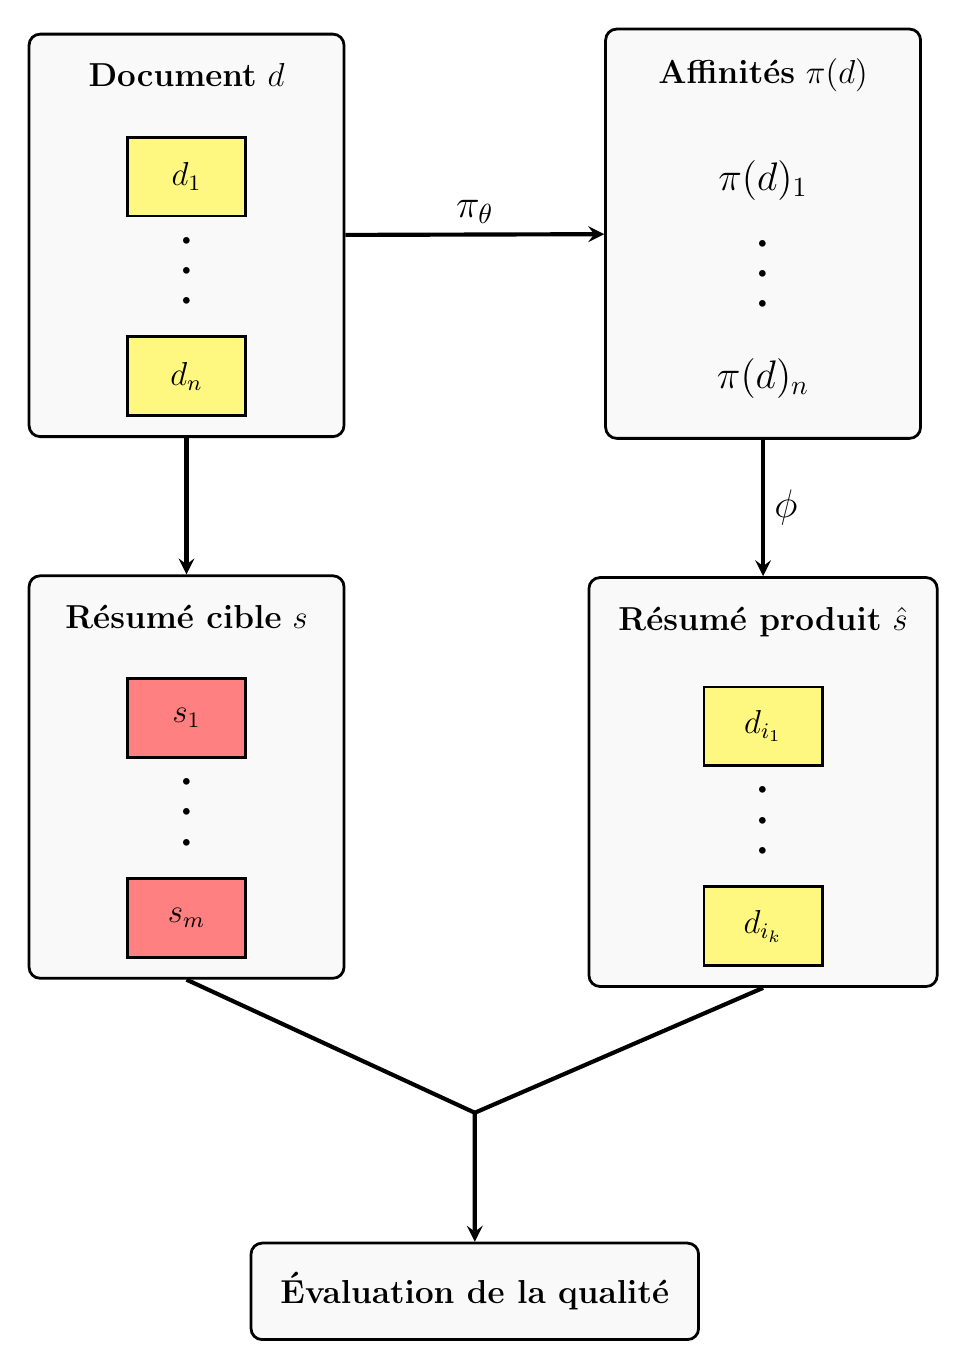
\begin{tikzpicture}[node distance=4.5cm, font=\large]
            \tikzstyle{default} = [rectangle, rounded corners, minimum width=4cm, minimum height=1cm, text centered, draw=black, line width=1pt, fill=gray!5, inner sep=0.25cm];
            \tikzstyle{sent} = [rectangle, minimum width=1.5cm, minimum height=1cm, text centered, draw=black, line width=1pt, fill=yellow!50, node distance=0.5cm];
            \tikzstyle{arrow} = [very thick,->,>=stealth, line width=1.5pt];
            
            \node (doc_t) {\textbf{Document} $d$};
            \node (d1) [sent, below=of doc_t] {$d_1$};
            \node (dn) [sent, below=of d1, yshift=-1cm] {$d_n$};
            \path (d1) -- (dn) node [font=\Huge, midway, sloped] {$\dots$};
            \begin{scope}[on background layer]
                \node (doc) [default, fit={(doc_t) (dn)}] {};
            \end{scope}
            
            \node (distro_t) [right=of doc_t]  {\textbf{Affinités} $\pi(d)$};
            \node (pi1) [node distance=0.5cm, minimum height=1cm, below=of distro_t] {\Large $\pi(d)_1$};
            \node (pin) [node distance=0.5cm, minimum height=1cm, below=of pi1, yshift=-1cm] {\Large $\pi(d)_n$};
            \path (pi1) -- (pin) node [font=\Huge, midway, sloped] {$\dots$};
            \begin{scope}[on background layer]
                \node (distro) [default, fit={(distro_t) (pin)}] {};
            \end{scope}
            
            \node (resume_t) [node distance=2cm, below=of distro] {\textbf{Résumé produit} $\hat{s}$};
            \node (di1) [sent, below=of resume_t] {$d_{i_1}$};
        \node (dik) [sent, below=of di1, yshift=-1cm] {$d_{i_k}$};
        \path (di1) -- (dik) node [font=\Huge, midway, sloped] {$\dots$};
        \begin{scope}[on background layer]
            \node (resume) [default, fit={(resume_t) (dik)}] {};
        \end{scope}
        
        \node (cible_t) [node distance=2cm, below=of doc] {\textbf{Résumé cible} $s$};
        \node (s1) [sent, fill=red!50, below=of cible_t] {$s_1$};
        \node (sm) [sent, fill=red!50, below=of s1, yshift=-1cm] {$s_m$};
        \path (s1) -- (sm) node [font=\Huge, midway, sloped] {$\dots$};
        \begin{scope}[on background layer]
            \node (cible) [default, fit={(cible_t) (sm)}] {};
        \end{scope}
        
        \coordinate (milieu) at ($(cible)!0.5!(resume)$);
        \node (eval_t) [below of = milieu, yshift=-2cm]  {\textbf{Évaluation de la qualité}};
        % \node (R) [node distance=0.5cm, minimum height=0.5cm, below=of eval_t] {\Large $\text{ROUGE}(\hat{s}, s)$};
        \begin{scope}[on background layer]
            \node (eval) [default, fit={(eval_t)}] {};
        \end{scope}
        
        \draw [arrow] (doc) -- node[anchor=south] {\Large $\pi_\theta$} (distro);
        \draw [arrow] (distro) -- node[anchor=west] {\Large $\phi$} (resume);
        \draw [arrow] (doc) -- node[anchor=west] {} (cible);
        
        \coordinate (milieu_bas) at ($(cible.south)!0.5!(resume.south)$);
        \coordinate (y) at ($(milieu_bas)!0.5!(eval.north)$);
        \draw [very thick,>=stealth, line width=1.5pt] (cible.south) -- (y);
        \draw [very thick,>=stealth, line width=1.5pt] (resume.south) -- (y);
        \draw [arrow] (y) -- (eval.north);
    \end{tikzpicture}
\end{center}
\caption[Processus de génération d'un résumé extractif]{Schéma des étapes de la génération de résumé extractif pour un document $d$ et 
son résumé cible $s$. La couleur différente utilisée pour les phrases du résumé 
cible sert à indiquer qu'elles ne sont habituellement pas des phrases du document
en entrée.}
\label{fig:summ}
\end{figure}

Enfin, pour un problème de génération de résumés donné, on fixe habituellement $\phi$.
L'objectif d'apprentissage est alors de trouver des paramètres $\theta$
qui permettent de maximiser la qualité des résumés produits par le modèle
$(\pi_\theta, \phi)$ à partir des paires document-résumé cibles $(d, s)$ contenues
dans un jeu de données $\mathcal{D}$.

\subsubsection*{Approches supervisées}

La majorité des approches extractives de l'état de l'art sont entraînées 
de manière supervisée à partir de cibles pour les affinités d'un document.
Or, comme le résumé $s$ correspondant à un document $d$ n'est habituellement pas obtenu de
manière extractive (i.e. le résumé n'est pas une combinaison de phrases du document initial),
il n'est pas trivial d'obtenir des cibles pour les affinités.
En pratique, les approches supervisées doivent utiliser des cibles basées sur des heuristiques pour
leur entraînement.

Par exemple, \citet{10.5555/3298483.3298681} précalculent des cibles binaires $y_d \in \{0,1\}^{|d|}$
utilisées comme cibles pour chaque document $d$.
Leurs cibles binaires représentent les phrases choisies par un oracle
sélectionnant de manière vorace les phrases $d_i \in d$ permettant de générer
un résumé extractif aussi près que possible du résumé cible $s$.
Après avoir sélectionné trois phrases, leur processus est arrêté et la cible $y_d$
d'un document $d$ est fixée à un vecteur binaire où les index des trois phrases 
retenues ont une valeur de 1 et les autres index ont une valeur nulle.

L'emploi de cibles binaires permet un entraînement supervisé très efficace:
\citet{liu2019text} utilisent seulement les cibles binaires
et représentent actuellement l'état de l'art extractif 
sur le populaire jeu de données du CNN/DailyMail \citep{hermann2015teaching}.
Notons toutefois qu'un réseau entraîné de manière supervisée à 
imiter un oracle ne peut pas obtenir une performance supérieure 
à celle de l'oracle.
Ainsi, les approches supervisées sont plus difficilement applicables
à des contextes où un bon oracle n'est pas disponible.

\subsubsection*{Approches par renforcement}
\label{subsec:rl_summ}

Au lieu d'utiliser des cibles binaires, les approches par renforcement visent à
optimiser directement une mesure numérique de la similarité entre deux résumés.
Disons que l'on dispose d'une métrique numérique de performance $G(\hat{s}, s)$
permettant de quantifier la proximité entre un résumé produit $\hat{s}$ et un résumé
cible $s$.
Il est alors possible de définir la fonction objective à maximiser
\begin{equation}
    J(\theta) = \underset{(d,s) \sim \mathcal{D}}{\mathbb{E}} \; \underset{\hat{s} \sim \phi(\pi_\theta(d))}{\mathbb{E}} \left[G(\hat{s}, s) \right],
    \label{eq:REINFORCE_expectation}
\end{equation}

représentant l'espérance de performance des résumés produits avec la paramétrisation $\theta$.
Comme on recherche $\theta^*$ maximisant $J(\theta)$, il vient naturellement en tête
de faire appel à des méthodes d'ascension de gradient\footnote{De manière analogue à
la descente de gradient présentée à la section \ref{subsec:gradient_descent} pour la minimisation
de fonction, l'ascension de gradient permet de maximiser une fonction.}.
Or, $J$ n'est pas calculable analytiquement en pratique car les deux espérances (sur
tous les documents et sur tous les résumés générables) sont habituellement intractables.

L'algorithme REINFORCE \citep{williams1992simple} propose une
solution élégante à ce problème, faisant une mise à jour des poids $\theta$ 
selon l'approximation du gradient de $J(\theta)$ basée sur un seul échantillon de $J$ 
\begin{equation}
    \nabla J(\theta) = G(\hat{s}, s)\nabla \ln \phi(\hat{s} | \pi_\theta, d), \quad d \sim \mathcal{D}, \hat{s} \sim \phi (\pi_\theta(d))
    \label{eq:REINFORCE_sample}
\end{equation}

où $\phi(\hat{s} | \pi_\theta, d)$ représente la probabilité de générer le résumé 
$\hat{s}$ à partir de $\pi_\theta(d)$ et $\phi$.


Le théorème du gradient de politique \citep{sutton1999policy} affirme que, en espérance,
l'approximation \eqref{eq:REINFORCE_sample} correspond au gradient de \eqref{eq:REINFORCE_expectation}
et peut donc être utilisée pour une ascension de gradient.
Les approches par renforcement basées sur REINFORCE \citep{dong2018banditsum,luo-etal-2019-reading}
parviennent actuellement à atteindre des performances très près de l'état
de l'art pour la génération automatique de résumés à un coût de calcul 
nettement inférieur.

\subsection{Formulation abstractive}

Sous cette formulation, on génère le résumé d'un texte un mot à la fois.
Les résumés abstractifs peuvent donc potentiellement reproduire 
de manière parfaite le résumé cible associé à un document.
Cette performance potentielle vient toutefois à un coût:
la formulation abstractive est naturellement plus difficile car elle nécessite de
gérer la syntaxe et les fautes d'orthographe en plus de la tâche 
de trouver les informations pertinentes du document.
De surcroît, les modèles abstractifs peuvent aussi être sujets à la génération 
d'énoncés factuellement incorrects \citep{kryscinski2020evaluating} .

Comme on s'intéresse aux méthodes extractives pour le reste du document,
on se contente de référer le lecteur aux approches abstractives
représentant l'état de l'art \citep{dou2020gsum, 2020t5, unilm, zhang2019pegasus}.
Au coeur de toutes ces approches se trouvent les architectures BERT 
\citep{devlin-etal-2019-bert} et Transformer \citep{vaswani2017attention},
auxquelles sont dues les percées récentes dans le domaine de la génération 
de texte.

\subsection{Évaluation de la performance}
\label{sec:rouge}

À la section \ref{sec:extractive}, on prenait pour acquis qu'une fonction $G$ existait
pour mesurer la proximité entre un résumé généré $\hat{s}$ et un résumé cible $s$.
Il en existe en fait plusieurs, notamment :

\begin{itemize}
    \item ROUGE-$n$ \citep{lin-2004-rouge}: métrique basée sur le chevauchement entre les séquences de $n$ mots ($n$-grammes)
          de $\hat{s}$ et $s$. Par exemple, $\text{ROUGE-1}$ représente le chevauchement entre les unigrammes
          et $\text{ROUGE-2}$ celui entre les bigrammes;
    \item ROUGE-L \citep{lin-2004-rouge}: métrique mesurant la plus longue sous-séquence commune
          entre $\hat{s}$ et;
    \item ROUGE-WE \citep{ng-abrecht-2015-better}: métrique similaire à ROUGE-$n$, mais qui utilise
          le \textit{soft-matching} basé sur la similarité entre les plongements de mots au lieu
          de la correspondance exacte.
\end{itemize}
L'intuition ici est simple: plus le chevauchement est grand entre les 
\ngrams d'un résumé généré et ceux du résumé cible, plus le résumé
généré a conservé l'information recherchée.

Or, si on se fie seulement au rappel sur les \textit{n}-grammes, le résumé optimal sera
de conserver tout le texte original. 
Pour pénaliser les résumés trop peu concis, on peut utiliser une métrique plus
appropriée que le rappel comme le score F1 pour pénaliser les 
\ngrams présents dans le résumé généré mais pas dans la cible.
Pour tout le document, tous les scores basés sur ROUGE rapportés seront donc 
basés sur la métrique F1.

Bien que ces métriques soient généralement
corrélées avec l'avis d'un expert humain, elles peuvent difficilement être considérées
comme un remplacement de celui-ci \citep{peyrard-2019-studying}.
En effet, comme les métriques sont toutes similairement corrélées avec le jugement humain
mais qu'elles ne sont que faiblement corrélées entre elles, aucune des métriques
ne peut être utilisée à elle seule comme un remplacement de l'avis humain.
En utilisant une moyenne de plusieurs métriques, il est possible d'alléger quelque peu
ce problème.
Notons toutefois que l'utilisation d'une moyenne ne suffit pas à régler le problème
en entier.
Par exemple, \citet{DBLP:journals/corr/PaulusXS17} entraînent 
plusieurs modèles abstractifs mais finissent par déployer un modèle n'atteignant
pas la meilleure moyenne de score ROUGE-1, ROUGE-2 et ROUGE-L après
une évaluation de la qualité des modèles par des humains.

Enfin, il est aussi important de mentionner que toutes les métriques énoncées 
plus haut ne sont pas dérivables.
Elles ne peuvent donc pas être utilisées directement comme fonctions de perte
pour l'entraînement d'un réseau de neurones.

\subsubsection*{Évaluation de la performance à partir d'un jeu de données}

On termine en mentionnant que, dans le contexte où l'on apprend à partir 
d'un jeu de données $\mathcal{D}=\{(d_i, s_i)\}_{i=1}^N$, il est important 
de faire l'évaluation sur un jeu de données différent de celui utilisé pour l'entraînement.
En effet, comme on s'intéresse à la performance d'un modèle de génération 
de résumés sur n'importe quel document en entrée, il est nécessaire de valider 
la performance du modèle sur des documents qui n'ont pas encore été vus par 
le modèle.

À cet effet, on sépare habituellement le jeu de données $\mathcal{D}$ en trois
sous-ensembles: un ensemble d'entraînement, un ensemble de validation et un ensemble 
de test.
L'ensemble d'entraînement est naturellement utilisé pour l'apprentissage du modèle
alors que l'ensemble de validation est utilisé pour estimer la performance 
sur des nouveaux documents pendant l'entraînement.
À la fin de l'entraînement, le modèle retenu est celui ayant la meilleure performance 
sur le jeu de validation.
Enfin, l'ensemble de test est utilisé pour estimer la performance réelle 
du modèle retenu. 

\chapter{Problématique}
\label{chap:bandit_contextuel}

L'objectif fondamental de ce mémoire est de proposer et 
d'analyser différents algorithmes basés 
sur les bandits pour l'apprentissage de systèmes de génération 
de résumés.
Pour atteindre cet objectif, il est essentiel de se doter 
d'un cadre expérimental qui sera réutilisé pour tous les algorithmes
testés afin de bien pouvoir attribuer les variations de performance 
aux algorithmes à l'essai.
On commence donc en présentant et motivant 
la problématique de génération de résumés à l'étude, avec toutes 
les contraintes et hypothèses retenues.

On présente ensuite BanditSum \citep{dong2018banditsum}, la première 
approche par bandit de ce document.
On voit comment BanditSum aborde la génération de tous les documents 
d'un ensemble comme un bandit contextuel \citep{contextual_bandits}.
On décrit par la suite comment l'algorithme REINFORCE \citep{williams1992simple} 
peut être utilisé pour résoudre le bandit contextuel proposé et 
on justifie son applicabilité à partir d'un ensemble de documents de développement.
Enfin, on met BanditSum à l'essai sur le jeu de données du CNN/DailyMail \citep{hermann2015teaching}  
et on fait valoir que la performance obtenue représente l'état de l'art
en termes d'efficacité computationnelle.

\section{Description}
\label{section:problematique}

La problématique à laquelle on s'intéresse est de trouver 
des approches par bandit qui permettent l'entraînement 
de modèles de génération de résumés.
Pour les travaux de ce document, il est choisi de s'intéresser exclusivement
aux résumés extractifs (voir section \ref{sec:extractive}), qui sont bâtis
en sélectionnant des phrases d'un document.
C'est la formulation extractive qui est retenue 
en raison de la facilité avec laquelle la génération de ce type 
de résumé peut être vue comme un problème de bandit.

Comme le résumé cible $s$ associé à un document $d$ est 
rarement constitué intégralement de phrases prélevées de $d$, il n'est pas trivial 
de définir une procédure d'apprentissage dans le contexte extractif.
En voyant la génération de résumés\footnote{À partir de maintenant, comme on considère exclusivement les 
résumés extractifs, on utilisera résumé et résumé extractif
de manière interchangeable.} comme un problème de bandit, on peut faire appel 
aux algorithmes connus de résolution des bandits pour 
optimiser les résumés produits par un modèle.
Pour la problématique à l'étude, on considère deux niveaux d'application des bandits: 
sur un ensemble de documents et sur un seul document à la fois.
Au niveau d'un ensemble de documents,
on parlera d'un objectif d'optimisation de la performance espérée du modèle 
alors qu'au niveau d'un document, on parlera plutôt d'un objectif de production 
de cibles de qualité.

Le coeur de ce document repose dans l'analyse de procédures 
d'apprentissage pour ces deux objectifs.
On se dote d'un cadre uniformisé pour comparer sur un pied d'égalité
les différents algorithmes explorés.
On fixe donc un jeu de données, une métrique d'évaluation 
et un modèle de réseau de neurones, tous largement inspirés
de BanditSum, la première approche par bandit proposée
dans la litérature pour 
l'entraînement de modèles de génération de résumés.


\subsection{Jeu de données}
\label{subsec:jeu_donnees}

Pour évaluer la performance des approches proposées, le jeu de données du
CNN/DailyMail \citep{hermann2015teaching}, référence classique dans le milieu
de la génération de résumés, sera utilisé.
Celui-ci est composé de plus de 300 000 articles de journaux et
leurs résumés écrits par un expert humain, séparés en 
287 113 exemples d'entraînement, 13 368 exemples de validation 
et 11 490 exemples de test.
Afin de mener des expériences empiriques plus poussées sur l'applicabilité
des différentes approches par bandit proposées, on utilise aussi un sous-ensemble 
du jeu d'entraînement comme jeu de développement.
Ce jeu de développement est composé de 25 000 exemples pigés 
aléatoirement du jeu d'entraînement afin d'être aussi varié que possible.
Notamment, il contient 8 674 documents de 20 phrases ou moins, 10 490
documents contenant entre 20 et 35 phrases exclusivement et 5 796 documents 
de 35 phrases ou plus.

De plus, une référence souvent utilisée pour ce jeu de données est l'heuristique
Lead-3 \citep{10.5555/3298483.3298681} qui consiste à générer le résumé d'un 
document à partir de ses 3 premières phrases.
En raison de sa bonne performance sur le jeu de données,
Lead-3 est généralement considérée comme une référence plancher pour la performance 
des modèles de génération de résumés.
En effet, comme l'heuristique Lead-3 ne requiert aucun temps d'entraînement 
ou ressource de calcul dédiée, n'importe quel modèle entraîné qui ne 
dépasse pas sa performance est considéré comme peu pertinent.

On emploie aussi plusieurs des contraintes retenues par les approches
de l'état de l'art sur le jeu de données du CNN/DailyMail.
Notamment, on considère exclusivement les résumés
de 3 phrases en sortie.
Cette contrainte, utilisée fréquemment sur le jeu de données du CNN/DailyMail,
est basée sur le fait que la moyenne du nombre de phrases contenues dans les résumés cibles
est près de 3.
De surcroît, les résultats obtenus par Lead-3 sont très bons aux yeux des métriques automatiques,
justifiant encore une fois qu'avec 3 phrases on peut générer de bons résumés des documents du jeu
de données.
Selon les statistiques du jeu de données, on considère aussi la régularisation
qui consiste à conserver seulement les documents d'au moins 3 phrases, limiter la taille des documents à
50 phrases au maximum et celle des phrases à 80 mots.
En cas d'excès de mots ou de phrases, l'excédent est simplement retiré.


\subsection{Métrique d'évaluation}
\label{subsec:eval}

Pour l'évaluation de la performance, on emploie les métriques ROUGE \citep{lin-2004-rouge}
présentées à la section \ref{sec:rouge}.
On retient la métrique de similarité entre deux résumés
utilisée par la plupart des travaux employant l'apprentissage par renforcement 
\citep{DBLP:journals/corr/PaulusXS17,dong2018banditsum,luo-etal-2019-reading}
\begin{equation}
    \text{ROUGE}(\hat{s}, s) := \frac{1}{3} \left[ \text{ROUGE-1}(\hat{s}, s) + \text{ROUGE-2}(\hat{s}, s) + \text{ROUGE-L}(\hat{s}, s) \right].
    \label{eq:ROUGE}
\end{equation}
Ici, ROUGE-1 et ROUGE-2 représentent respectivement le chevauchement au niveau des unigrammes 
et des bigrammes entre $\hat{s}$ et $s$ alors que ROUGE-L mesure leur plus longue 
sous-séquence commune.
Toutes les métriques utilisées sont 
basées sur le score F1 afin de pénaliser les résumés trop longs, 
tel que mentionné à la section \ref{sec:rouge}.

Notons que le choix de \eqref{eq:ROUGE} comme métrique d'évaluation est motivé par deux facteurs principaux.
D'abord, ROUGE\footnote{Ici et dans le reste du document, 
ROUGE représente la métrique définie par l'équation \eqref{eq:ROUGE}.} jouit d'une diversité de signal naturelle 
comme il s'agit de la moyenne de trois métriques différentes.
C'est cette diversité de signal
qui permet d'avoir une évaluation automatique se rapprochant le plus
possible de l'évaluation humaine.
Aussi, le score ROUGE a la propriété intéressante d'être presque invariant 
à l'ordre des phrases dans un résumé: seul le score $\text{ROUGE-2}$ est 
modifié au niveau de la jonction entre deux phrases quand l'ordre 
des phrases varie.
On exploite abondamment cette propriété car elle permet d'éviter 
l'explosion combinatoire induite par la considération de l'ordre 
des phrases dans un résumé.
Notamment, pour un groupe de 3 phrases composant un résumé, 
on assigne toujours le score ROUGE associé au résumé où les phrases 
apparaîssent dans le même ordre que dans le document original.

\subsubsection*{Pré-calcul des scores ROUGE}

Les méthodes présentées dans ce document font toutes
appel au calcul de plusieurs scores ROUGE dans leur procédure d'entraînement.
Comme les calculs de ROUGE sont plutôt lents et que l'on souhaite 
éviter qu'ils deviennent le principal fardeau computationnel, 
on effectue le pré-calcul des scores pour tous les documents du jeu 
d'entraînement.
Pour un document $d$, on sait que tous les résumés que l'on doit considérer sont 
les combinaisons de 3 phrases ordonnées selon leur position initiale dans $d$.
Il est donc possible de calculer et entreposer le score $\text{ROUGE}(\hat{s}, s)$ 
de tous les résumés $\hat{s}$ d'un document et de simplement aller lire la valeur 
correspondante lorsque nécessaire dans l'entraînement.

\subsection{Architecture neuronale}
\label{subsec:archi}

Au niveau architectural, on reprend exactement le modèle neuronal
de BanditSum, pour lequel une illustration est disponible à la 
figure \ref{fig:archi}.
Le modèle obtient d'abord une représentation de chaque phrase 
en prenant la moyenne des sorties d'un LSTM bidirectionnel 
à deux couches appliqué sur les plongements de mots.
Ces représentations sont ensuite passées à un second LSTM bidirectionnel
à deux couches, lequel produit des représentations de chaque phrase
qui tiennent compte des autres phrases du document.
Les affinités sont finalement obtenues via une tête de prédiction
constituée d'un réseau pleinement connecté
composé de deux couches reliées par une activation ReLU et avec sortie 
sigmoïde.
Ici, la fonction sigmoïde est utilisée car elle permet d'avoir une sortie 
entre 0 et 1 que l'on interprète comme l'affinité prédite par le modèle 
pour l'inclusion d'une phrase dans le résumé.
À l'inférence, un résumé est produit en sélectionnant les 
3 phrases avec la plus grande affinité.
On utilisera exactement la même architecture de réseau de neurones pour toutes
les expérimentations de ce document.

\tikzsetnextfilename{tikz_archi}
\begin{figure}[ht!]
    \centering
    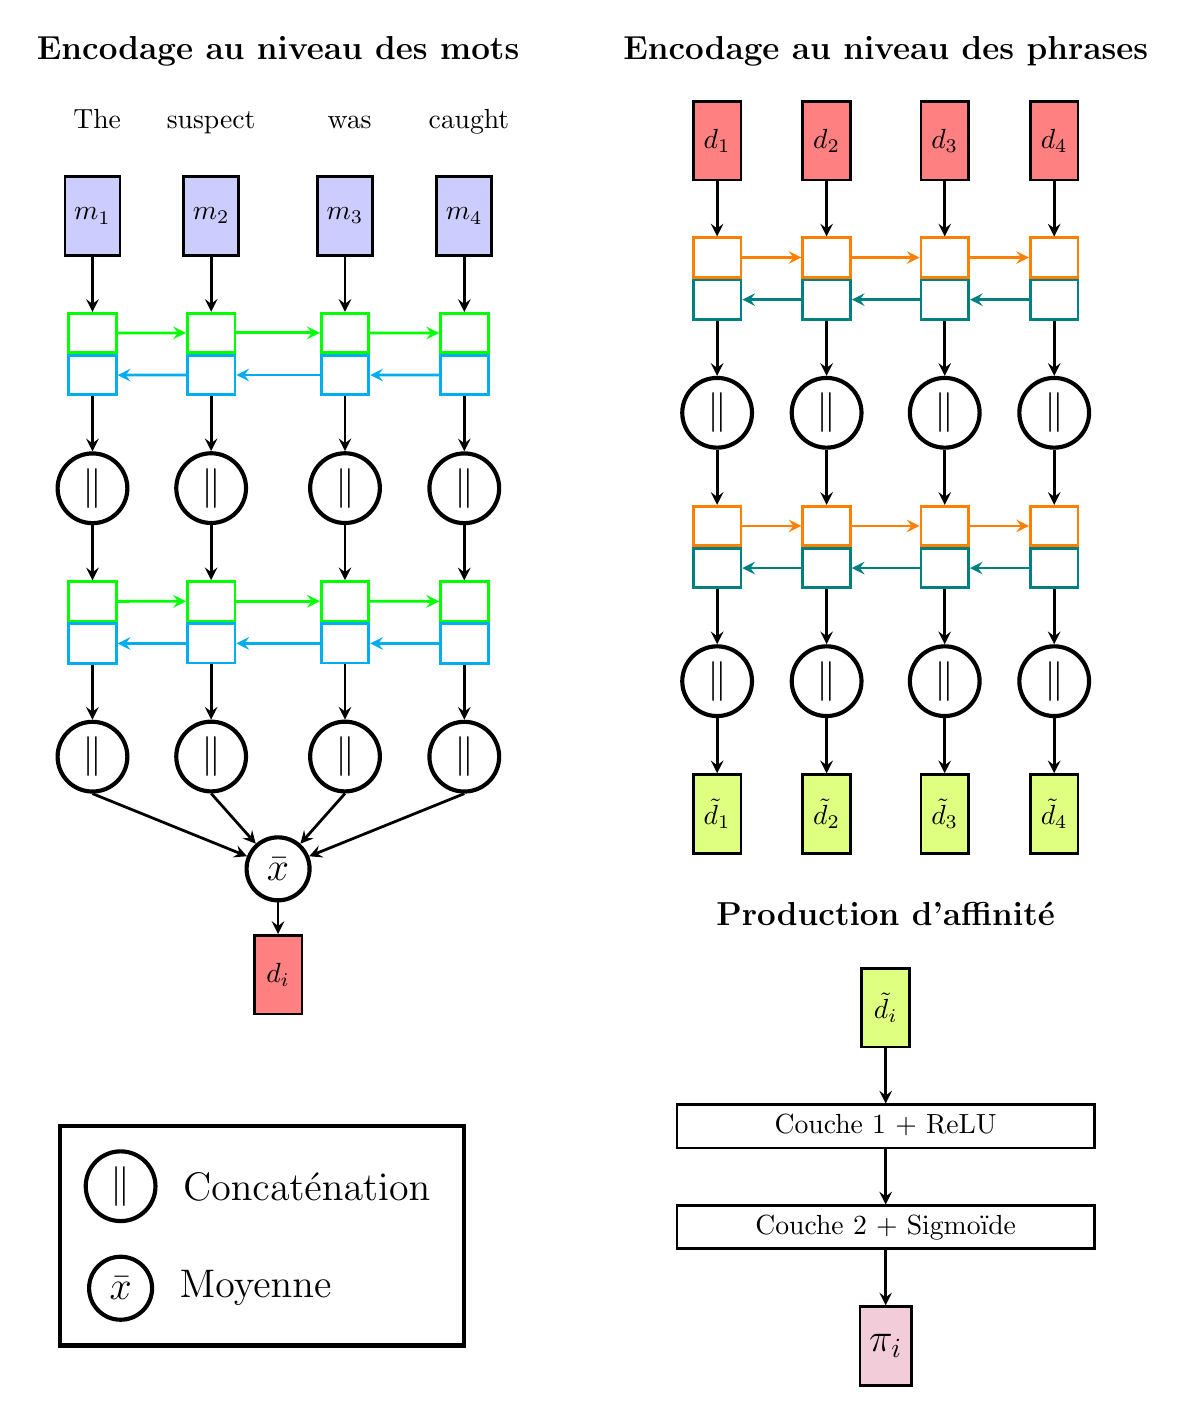
\begin{tikzpicture}[node distance=0.7cm]
        \tikzstyle{default} = [rectangle, text centered, draw=black, line width=1pt];
        \tikzstyle{embedding} = [default, minimum width=width("The"), minimum height=1.0cm, fill=blue!20, node distance=0.4cm];
        \tikzstyle{word} = [minimum width=width("caught"), minimum height=height("The"), node distance=0.3cm];
        \tikzstyle{arrow} = [very thick,->,>=stealth, line width=1pt];
        \tikzstyle{cell} = [default, minimum height=0.5cm, minimum width=width("The"), draw=green];
        \tikzstyle{cellb} = [cell, draw=cyan];
        \tikzstyle{arrowf} = [arrow, draw=green];
        \tikzstyle{arrowb} = [arrow, draw=cyan];
        \tikzstyle{operation} = [default, circle, minimum width=0.8cm, line width=1.5pt];

        % Word-level encoding
        \node (titre1) [font=\large] {\textbf{Encodage au niveau des mots}};
        \node (was) [word, below=0.3cm of titre1, xshift=0.85cm] {\vphantom{Ty} was};
        \node (suspect) [word, below=0.3cm of titre1, xshift=-0.85cm] {\vphantom{Ty}suspect};
        \node (the) [word, left=of suspect] {\vphantom{Ty} The};
        \node (caught) [word, right=of was] {\vphantom{Ty} caught};

        % Word embeddings
        \node (m1) [embedding, below=of the] {$m_1$}; 
        \node (m2) [embedding, below=of suspect] {$m_2$}; 
        \node (m3) [embedding, below=of was] {$m_3$}; 
        \node (m4) [embedding, below=of caught] {$m_4$}; 

        % First LSTM layer
        \node (h11f) [cell, below=of m1] {};
        \node (h11b) [cellb, below=0cm of h11f.south] {};
        \node (h12f) [cell, below=of m2] {};
        \node (h12b) [cellb, below=0cm of h12f.south] {};
        \node (h13f) [cell, below=of m3] {};
        \node (h13b) [cellb, below=0cm of h13f.south] {};
        \node (h14f) [cell, below=of m4] {};
        \node (h14b) [cellb, below=0cm of h14f.south] {};
       
        \draw [arrow] (m1) -- (h11f);
        \draw [arrow] (m2) -- (h12f);
        \draw [arrow] (m3) -- (h13f);
        \draw [arrow] (m4) -- (h14f);

        \draw [arrowf] (h11f) -- (h12f);
        \draw [arrowf] (h12f) -- (h13f);
        \draw [arrowf] (h13f) -- (h14f);

        \draw [arrowb] (h14b) -- (h13b);
        \draw [arrowb] (h13b) -- (h12b);
        \draw [arrowb] (h12b) -- (h11b);

        % Concatenation Layer
        \node (cat1) [operation, below=of h11b] {\Large $\Vert$};
        \node (cat2) [operation, below=of h12b] {\Large $\Vert$};
        \node (cat3) [operation, below=of h13b] {\Large $\Vert$};
        \node (cat4) [operation, below=of h14b] {\Large $\Vert$};

        \draw [arrow] (h11b) -- (cat1);
        \draw [arrow] (h12b) -- (cat2);
        \draw [arrow] (h13b) -- (cat3);
        \draw [arrow] (h14b) -- (cat4);

        % Second LSTM Layer
        \node (h21f) [cell, below=of cat1] {};
        \node (h21b) [cellb, below=0cm of h21f.south] {};
        \node (h22f) [cell, below=of cat2] {};
        \node (h22b) [cellb, below=0cm of h22f.south] {};
        \node (h23f) [cell, below=of cat3] {};
        \node (h23b) [cellb, below=0cm of h23f.south] {};
        \node (h24f) [cell, below=of cat4] {};
        \node (h24b) [cellb, below=0cm of h24f.south] {};

        \draw [arrow] (cat1) -- (h21f);
        \draw [arrow] (cat2) -- (h22f);
        \draw [arrow] (cat3) -- (h23f);
        \draw [arrow] (cat4) -- (h24f);

        \draw [arrowf] (h21f) -- (h22f);
        \draw [arrowf] (h22f) -- (h23f);
        \draw [arrowf] (h23f) -- (h24f);

        \draw [arrowb] (h24b) -- (h23b);
        \draw [arrowb] (h23b) -- (h22b);
        \draw [arrowb] (h22b) -- (h21b);

        \node (cat6) [operation, below=of h21b] {\Large $\Vert$};
        \node (cat7) [operation, below=of h22b] {\Large $\Vert$};
        \node (cat8) [operation, below=of h23b] {\Large $\Vert$};
        \node (cat9) [operation, below=of h24b] {\Large $\Vert$};

        \draw [arrow] (h21b) -- (cat6);
        \draw [arrow] (h22b) -- (cat7);
        \draw [arrow] (h23b) -- (cat8);
        \draw [arrow] (h24b) -- (cat9);

        % Mean of LSTM outputs
        \coordinate (milieu_cat) at ($(cat7)!0.5!(cat8)$);
        \node (mean) [operation, below=1cm of milieu_cat] {\Large $\bar x$};
        
        \draw [arrow] (cat6.south) -- (mean);
        \draw [arrow] (cat7.south) -- (mean);
        \draw [arrow] (cat8.south) -- (mean);
        \draw [arrow] (cat9.south) -- (mean);

        \tikzstyle{sent} = [embedding, fill=red!50];
        
        \node (di) [sent, below=of mean] {$d_i$};
        
        \draw [arrow] (mean) -- (di);
        
        \coordinate (barre_haut) at ([xshift = 0.5cm]caught.east |- titre1.north);
        \coordinate (barre_bas) at ([xshift = 0.5cm]caught.east |- di.south);

        % \draw [line width=2pt] (barre_haut) -- (barre_bas);

        \tikzstyle{cell} = [default, minimum height=0.5cm, minimum width=width("The"), draw=orange];
        \tikzstyle{cellb} = [cell, draw=teal];
        \tikzstyle{arrowf} = [arrow, draw=orange];
        \tikzstyle{arrowb} = [arrow, draw=teal];

        % Sentence-level encoding
        \node (titre2) [font=\large, right=of barre_haut, anchor=north west] {\textbf{Encodage au niveau des phrases}};
        \node (d2) [sent, below=0.3cm of titre2, xshift=-0.75cm] {$d_2$};
        \node (d3) [sent, below=0.3cm of titre2, xshift=0.75cm] {$d_3$};
        \node (d1) [sent, left=0.75cm of d2] {$d_1$};
        \node (d4) [sent, right=0.75cm of d3] {$d_4$};

        % % First LSTM layer
        \node (h31f) [cell, below=of d1] {};
        \node (h31b) [cellb, below=0cm of h31f.south] {};
        \node (h32f) [cell, below=of d2] {};
        \node (h32b) [cellb, below=0cm of h32f.south] {};
        \node (h33f) [cell, below=of d3] {};
        \node (h33b) [cellb, below=0cm of h33f.south] {};
        \node (h34f) [cell, below=of d4] {};
        \node (h34b) [cellb, below=0cm of h34f.south] {};
       
        \draw [arrow] (d1) -- (h31f);
        \draw [arrow] (d2) -- (h32f);
        \draw [arrow] (d3) -- (h33f);
        \draw [arrow] (d4) -- (h34f);

        \draw [arrowf] (h31f) -- (h32f);
        \draw [arrowf] (h32f) -- (h33f);
        \draw [arrowf] (h33f) -- (h34f);

        \draw [arrowb] (h34b) -- (h33b);
        \draw [arrowb] (h33b) -- (h32b);
        \draw [arrowb] (h32b) -- (h31b);

        % % Concatenation Layer
        \node (cat11) [operation, below=of h31b] {\Large $\Vert$};
        \node (cat12) [operation, below=of h32b] {\Large $\Vert$};
        \node (cat13) [operation, below=of h33b] {\Large $\Vert$};
        \node (cat14) [operation, below=of h34b] {\Large $\Vert$};

        \draw [arrow] (h31b) -- (cat11);
        \draw [arrow] (h32b) -- (cat12);
        \draw [arrow] (h33b) -- (cat13);
        \draw [arrow] (h34b) -- (cat14);

        % % Second LSTM Layer
        \node (h41f) [cell, below=of cat11] {};
        \node (h41b) [cellb, below=0cm of h41f.south] {};
        \node (h42f) [cell, below=of cat12] {};
        \node (h42b) [cellb, below=0cm of h42f.south] {};
        \node (h43f) [cell, below=of cat13] {};
        \node (h43b) [cellb, below=0cm of h43f.south] {};
        \node (h44f) [cell, below=of cat14] {};
        \node (h44b) [cellb, below=0cm of h44f.south] {};

        \draw [arrow] (cat11) -- (h41f);
        \draw [arrow] (cat12) -- (h42f);
        \draw [arrow] (cat13) -- (h43f);
        \draw [arrow] (cat14) -- (h44f);

        \draw [arrowf] (h41f) -- (h42f);
        \draw [arrowf] (h42f) -- (h43f);
        \draw [arrowf] (h43f) -- (h44f);

        \draw [arrowb] (h44b) -- (h43b);
        \draw [arrowb] (h43b) -- (h42b);
        \draw [arrowb] (h42b) -- (h41b);

        \node (cat16) [operation, below=of h41b] {\Large $\Vert$};
        \node (cat17) [operation, below=of h42b] {\Large $\Vert$};
        \node (cat18) [operation, below=of h43b] {\Large $\Vert$};
        \node (cat19) [operation, below=of h44b] {\Large $\Vert$};

        \draw [arrow] (h41b) -- (cat16);
        \draw [arrow] (h42b) -- (cat17);
        \draw [arrow] (h43b) -- (cat18);
        \draw [arrow] (h44b) -- (cat19);

        \tikzstyle{sent2} = [embedding, fill=lime!50];

        \node (d1t) [sent2, below=0.7cm of cat16] {$\tilde{d}_1$};
        \node (d2t) [sent2, below=0.7cm of cat17] {$\tilde{d}_2$};
        \node (d3t) [sent2, below=0.7cm of cat18] {$\tilde{d}_3$};
        \node (d4t) [sent2, below=0.7cm of cat19] {$\tilde{d}_4$};

        \draw [arrow] (cat16) -- (d1t);
        \draw [arrow] (cat17) -- (d2t);
        \draw [arrow] (cat18) -- (d3t);
        \draw [arrow] (cat19) -- (d4t);

        \coordinate (milieu_dt) at ($(d2t)!0.5!(d3t)$);

        \tikzstyle{layer} = [default, minimum width=5.3cm, minimum height=height("Sigmoïde")];
        \node (titre3) [below=1cm of milieu_dt] {\large \textbf{Production d'affinité}};
        \node (dit) [sent2, below=of titre3] {$\tilde{d}_i$};
        \node (fc1) [layer, below=of dit] {\vphantom{Sg}Couche 1 + ReLU};
        \node (fc2) [layer, below=of fc1] {\vphantom{Sg}Couche 2 + Sigmoïde};
        \node (aff) [sent, fill=purple!20, below=0.7cm of fc2] {\Large $\pi_i$};

        \draw [arrow] (dit) -- (fc1);
        \draw [arrow] (fc1) -- (fc2);
        \draw [arrow] (fc2) -- (aff);

        \node (cat) [operation, below=1.7cm of di, xshift=-2cm] {\Large $\Vert$};
        \node (cat_d) [right=0.2cm of cat] {\Large Concaténation};
        \node (mean_leg) [operation, below=0.4cm of cat] {\Large $\bar x$};
        \node (mean_d) [right=0.2cm of mean_leg] {\Large Moyenne};
        \node (legende) [rectangle, line width=1.5pt, draw=black, inner sep=0.3cm, fit={(cat) (cat_d) (mean_leg) (mean_d)}] {};
    \end{tikzpicture}
    \caption[Architecture neuronale de BanditSum]
    {Schéma décrivant l'architecture neuronale employée par BanditSum et reprise pour 
    les expérimentations tout au long du document.
    On présente tout le parcours interne des deux LSTMs bidirectionnels à deux 
    couches.
    Les représentations de phrases à partir de leurs mots sont en rouge et les 
    représentations incorporant les autres phrases sont en vert pâle.}
    \label{fig:archi}
\end{figure}

\subsubsection*{Détails expérimentaux}

On reprend des détails d'implémentation 
identiques à BanditSum afin de faciliter 
la comparaison avec les autres approches par bandit.
La dimension cachée des LSTMs est fixée à 200
et celle de la tête de prédiction est de 100.
Les plongements de mots utilisés sont les plongements GLoVe \citep{pennington2014glove} de taille 100 
pré-entraînés sur la langue anglaise.
On retient seulement les plongements pour les mots présents au moins une fois 
dans le jeu d'entraînement.
Pour tous les mots pour lesquels on ne dispose pas de plongement 
(mots hors vocabulaire), on utilise un même plongement 
aléatoire partagé.
L'optimiseur employé est Adam \citep{kingma2014method}, pour lequel on fixe 
$\beta = [0, 0.999]$.
On utilise un taux d'apprentissage $\alpha=5e^{-5}$ et une pénalité sur la norme 
des poids $\theta$ de $1e^{-6}$.
Un \textit{gradient clipping} de 1 est aussi appliqué.

Tous les entraînements sont faits en itérant 
5 fois sur l'entièreté du jeu d'entraînement.
La taille de \textit{minibatch} utilisée pour la mise à jour 
des paramètres est $B=64$.
Toutes les expérimentations sont menées 
sur une carte graphique Tesla T4, dotée d'une mémoire 
virtuelle de 16 GB.

\section{Bandit contextuel}

Un bandit contextuel est une généralisation 
du problème de bandit stochastique présenté en \ref{subsec:bandit_stochastique}.
Dans cette formulation, à chaque pas de temps $t$ l'apprenant perçoit un 
contexte $c_t \in \mathcal{C}$, pour $\mathcal{C}$ l'ensemble des contextes possibles.
Ce contexte $c_t$ permet à l'apprenant de guider le choix de son action $a_t$,
à laquelle une récompense dépendante du contexte $X_{a_t,t} = r(c_t, a_t) + \xi_t$,
où $\xi_t$ est un bruit (e.g. supposé gaussien), est associée.
Comme il n'existe pas de contraintes sur le contexte utilisé, cette
formulation est très flexible et peut être utilisée pour n'importe quelle
tâche où le comportement optimal d'un apprenant est dépendant d'informations 
reçues en entrée.

\subsection{Application à la génération de résumés}
\label{subsec:context_gen_res}

La formulation contextuelle se prête naturellement à la génération 
de résumés pour un ensemble de documents que représente notre problématique (voir la section
 \ref{section:problematique}).
Pour une paire document-résumé $(d, s)$ d'un jeu de données, il suffit de définir le contexte
comme étant le document ($c=d$).
En génération de résumés, l'utilisation d'un document comme contexte correspond à l'hypothèse
facilement vérifiable que ce n'est pas nécessairement une bonne stratégie de 
toujours sélectionner les mêmes index de phrases d'un document pour bâtir son résumé.
En posant $\mathcal{S}_d$ comme étant l'ensemble des résumés
de 3 phrases de $d$, on a que les actions qui s'offrent à l'apprenant 
sont simplement les résumés $\hat{s} \in \mathcal{S}_d$.
Ainsi, la récompense $X_t$ per­çue au temps $t$ représente naturellement la valeur de
ROUGE associée $\text{ROUGE}(\hat{s}_t, s)$ au résumé $\hat{s}_t$ sélectionné
par l'apprenant au temps $t$.

L'introduction de la notion de contexte est 
cruciale dans le cas de la génération de résumés, 
car elle permet d'avoir un seul apprenant dont la 
tâche est de produire un résumé pour n'importe quel document $d$ en entrée.
Cet apprenant peut alors être n'importe quelle fonction paramétrée, 
un réseau de neurones par exemple, dont les paramètres $\theta$ 
sont appris dans l'objectif de maximisation de la performance
espérée sur tous les documents.

\subsection{REINFORCE pour maximisation de la performance espérée}
\label{section:echantillonnage}

Si l'on considère un apprenant $\pi_\theta$ doté d'une certaine paramétrisation $\theta$,
l'algorithme REINFORCE (\ref{subsec:rl_summ}) peut être utilisé pour 
maximiser $J(\theta)$ \eqref{eq:REINFORCE_expectation}, la récompense espérée en générant
un résumé à partir de $\pi_\theta$.
Selon le formalisme de génération de résumés défini à la section \ref{sec:extractive},
l'apprenant $\pi$ retourne des affinités de sélection $\pi(d) \in [0,1]^{|d|}$
pour chaque phrase d'un document $d$.

Dans ce contexte, il est alors naturel de vouloir utiliser un processus stochastique 
pour la génération de résumés, car cela permet une expressivité 
bien plus élevée pour $J$.
En effet, en sélectionnant les résumés de manière vorace (i.e. selon 
les 3 affinités maximales de $\pi(d)$), $J(\theta)$ devient une simple 
espérance sur la pige d'un document $d$, une mesure peu révélatrice 
de la performance globale de l'apprenant.
Toutefois, si l'on génère les résumés en pigeant sans remise dans 
la distribution $p(d)$ induite par $\pi(d)$, on permet à $J(\theta)$
de tenir compte de tous les résumés possibles de $d$, pondérés par leur probabilité de pige,
permettant de distinguer des distributions qui accordent une plus grande probabilité aux
meilleurs résumés.
Pour toutes les expériences de ce chapitre, on emploie donc le processus $\xi$ de génération stochastique de résumé
qui pige 3 phrases sans répétition selon la distribution induite par $\pi(d)$.

En pratique, les approximations de $\nabla J(\theta)$ nécessaires à la 
mise à jour de REINFORCE générées en utilisant un seul
échantillon de $J$ sont très instables pour un processus stochastique comme $\xi$,
rendant l'ascension de gradient \eqref{eq:REINFORCE_sample} difficile.
Une solution simple et peu coûteuse pour stabiliser l'entraînement est alors de piger $N$
résumés $\hat{s}_n$ en fonction de $\xi$ et $\pi_\theta$ pour bâtir un meilleur estimateur selon

\begin{equation}
    \nabla J(\theta) = \frac{1}{N} \sum_{n=1}^N \text{ROUGE}(\hat{s}_n, s) \nabla \ln \xi\left(\hat{s}_n| \pi_\theta, d\right).
    \label{eq:REINFORCE_samples}
\end{equation}

Ici, $\xi\left(\hat{s}_n| \pi_\theta, d\right)$ est la probabilité de produire le résumé $\hat{s}_n$
a partir de la distribution induite par $\pi_\theta(d)$ et du processus de génération stochastique
$\xi$ et ROUGE($\hat{s}_n$, $s$) est la similarité entre un résumé généré $\hat{s}_n$ et sa cible $s$.

\subsection{Expériences}

On s'intéresse à savoir combien d'échantillons sont requis pour obtenir une représentation 
adéquate de la valeur de $\nabla J(\theta)$.
On note d'abord que, dans l'équation \eqref{eq:REINFORCE_samples}, la dérivée de $\ln \xi(\pi)$ est déterministe
et n'est pas sensible à la portion stochastique du processus de génération de résumés.
Pour mesurer la qualité de l'approximation, il faut donc seulement s'intéresser
à la différence entre la véritable valeur de $J(\theta)$ et son estimation 
basée sur des échantillons selon $\xi(\pi)$.
Enfin, comme la pige d'un document $d$ dans le calcul de $J$ est uniforme, on
peut simplement s'intéresser à l'estimation de $J$ sur un seul document à la fois.

On prend donc $J$ comme étant l'espérance exacte de récompense de $\xi$ et de $\pi$ sur une paire 
document-résumé $(d, s)$ quelconque et on pose
$\bar{J}_N(\theta) =  \frac{1}{N} \sum_{n=1}^N \text{ROUGE}(\hat{s}_n, s)$, son approximation 
à partir de $N$ échantillons.
La qualité de l'échantillonnage dépend de la proximité entre $J$ et $\bar{J_N}$, que
l'on nomme l'erreur d'échantillonnage $\Delta_N$

\begin{equation}
    \Delta_N = \left| J(\theta) - \bar{J}_N(\theta) \right|.
    \label{eq:erreur_echantillonnage}
\end{equation}

\subsubsection*{Méthodologie}

On valide la rapidité de la convergence de $\bar{J}_N$ vers $J$ en les comparant
directement sur notre ensemble de développement (\ref{subsec:jeu_donnees}).
Comme le calcul de $\bar{J}_N$ requiert une distribution pour un document,
on génère artificiellement des distributions $p(d)$ sur les phrases d'un document $d$.
Pour assurer une bonne variété dans les distributions générées, on choisit des
distributions représentant une somme pondérée entre une distribution uniforme
$U(d)$ et une distribution vorace $G(d)$:

\begin{equation*}
    p(d) = \tau U(d) + (1 - \tau) G(d).
\end{equation*}

La distribution vorace employée $G(d)$ représente un vecteur de taille $|d|$ où trois indices 
pigés aléatoirement ont la valeur de $\frac{1}{3}$ et les autres indices sont nuls.
En jumelant ainsi des distributions vorace et uniforme selon un paramètre $\tau$,
les distributions générées $p(d)$ peuvent être arbitrairement plus faciles ou difficiles 
à estimer.
Plus $\tau$ est élevé, plus $p(d)$ sera près d'une distribution 
vorace, pour laquelle la pige stochastique est toujours identique et l'approximation 
ne requiert qu'un seul échantillon.

Les expériences consistent à calculer la valeur de $\Delta_N$ pour $N$ 
allant jusqu'à 50 sur tous les documents du jeu de développement.
Pour chaque document, on génère 100 distributions $p(d)$
en faisant varier $\tau$ de 0 à 1 en incréments de 0.01 et en repigeant les indices 
non-nuls de $G(d)$ à chaque fois.
Pour chaque distribution artificielle $p(d)$, les approximations $\bar{J}_N$ sont
calculées.
On calcule la véritable valeur de 
\begin{equation*}
    J = \mathop\mathbb{E}_{\hat{s} \sim \xi(p(d))} [\text{ROUGE}(\hat{s}, s)]
\end{equation*}
 grâce au fait que l'on possède
les scores ROUGE de tous les résumés extractifs de chacun des documents.

\subsection{Résultats}
\label{subsec:results_bs}

Les résultats obtenus sont rapportés dans les figures \ref{fig:bandit_contextuel_overall}
et \ref{fig:bandit_contextuel_top3} qui présentent respectivement
l'impact de la taille du document et de la distribution $p(d)$ employée
sur l'évolution de l'erreur d'échantillonnage $\Delta_N$.
Il est à noter que les différences rapportées entre les différentes 
courbes sur les figures ne sont pas statistiquement significatives.
Pour éviter d'encombrer inutilement les figures, on rapporte alors 
seulement les moyennes observées.
Les versions incorporant la déviation standard des différentes courbes 
se trouvent à l'annexe \ref{chap:variance_graphs}.

Tout d'abord, sur la figure \ref{fig:bandit_contextuel_overall}, 
on remarque que le nombre de phrases dans un document n'est pas un
facteur déterminant sur la rapidité de convergence de l'approximation par échantillonnage.
Ce résultat n'est pas surprenant: on peut s'attendre à ce que la difficulté
de convergence soit davantage qualifiée par une mesure sur la distribution
des résumés.

\tikzsetnextfilename{bandit_contextuel_overall}
\begin{figure}[ht!]
    \begin{center}
        \begin{tikzpicture}
            \begin{axis}[grid style={dashed,gray!50}, axis y line*=left, axis x line*=bottom, every axis plot/.append style={line width=1.5pt, mark size=0pt, font=\huge}, name=plot0, xshift=-.1\textwidth, ylabel={$\Delta_N$}, xlabel={Nombre $N$ d'échantillons}, width=0.95\textwidth, height=0.4\textwidth, smooth, xmin=1, xmax=50, y tick label style={/pgf/number format/fixed}, scaled y ticks = false, ytick={1, 2, 3, 4, 5}]
                \addplot[red, ylabel near ticks, line width=1.5pt] table[x expr=\thisrow{t} + 1, y expr=\thisrow{less20_} * 100, col sep=comma]{bandit_contextuel/bandit_contextuelExpResults/doc_len/all.csv};
                \addplot[green, ylabel near ticks, line width=1.5pt] table[x expr=\thisrow{t} + 1, y expr=\thisrow{20to35_} * 100, col sep=comma]{bandit_contextuel/bandit_contextuelExpResults/doc_len/all.csv};
                \addplot[blue, ylabel near ticks, line width=1.5pt] table[x expr=\thisrow{t} + 1, y expr=\thisrow{more35_} * 100, col sep=comma]{bandit_contextuel/bandit_contextuelExpResults/doc_len/all.csv};
                \legend{$|d| \leq 20$, $20 < |d| < 35$, $35 \leq |d|$}
            \end{axis}
        \end{tikzpicture}
    \end{center}
    \caption[Erreur d'échantillonnage selon la taille de document]
    {Impact de la taille du document en entrée sur l'erreur d'échantillonnage \eqref{eq:erreur_echantillonnage}
    (plus bas est meilleur).}
    \label{fig:bandit_contextuel_overall}
\end{figure}

Une mesure naturelle sur la distribution des résumés est la valeur maximale de
la distribution des résumés $\xi\left(p(d)\right)$.
La figure \ref{fig:bandit_contextuel_top3} montre une évolution à la tendance logarithmique
pour chaque nombre d'échantillons $N$ considérés,
où plus la probabilité maximale de la distribution augmente, plus rapide est la convergence
de notre processus d'échantillonnage.

\tikzsetnextfilename{bandit_contextuel_top3}
\begin{figure}[ht!]
    \begin{center}
        \begin{tikzpicture}
            \begin{axis}[legend cell align={left}, grid style={dashed,gray!50}, axis y line*=left, axis x line*=bottom, every axis plot/.append style={line width=1.5pt, mark size=0pt, font=\huge}, name=plot0, xshift=-.1\textwidth, y tick label style={/pgf/number format/fixed zerofill,
                /pgf/number format/precision=1,
                /pgf/number format/fixed}, ylabel={$\Delta_N$}, xlabel={Probabilité maximale de $\xi(p(d))$}, width=0.95\textwidth, height=0.4\textwidth, smooth, scaled y ticks = false, ymin=0.0, ymax=2.0, ytick={0.5, 1.0, 1.5, 2.0}, xmin=0.06, xmax=1.01]
                \addplot[red, ylabel near ticks, line width=1.5pt] table[x=t, y expr=\thisrow{t8_} * 100, col sep=comma]{bandit_contextuel/bandit_contextuelExpResults/top3/all.csv};
                \addplot[green, ylabel near ticks, line width=1.5pt] table[x=t, y expr=\thisrow{t16_} * 100, col sep=comma]{bandit_contextuel/bandit_contextuelExpResults/top3/all.csv};
                \addplot[blue, ylabel near ticks, line width=1.5pt] table[x=t, y expr=\thisrow{t32_} * 100, col sep=comma]{bandit_contextuel/bandit_contextuelExpResults/top3/all.csv};
                \addplot[yellow, ylabel near ticks, line width=1.5pt] table[x=t, y expr=\thisrow{t64_} * 100, col sep=comma]{bandit_contextuel/bandit_contextuelExpResults/top3/all.csv};
                \legend{$N=8$, $N=16$, $N=32$, $N=64$}
            \end{axis}
        \end{tikzpicture}
    \end{center}
    \caption[Erreur d'échantillonnage selon la plus grande probabilité de génération]
    {Impact de la probabilité maximale de la distribution des résumés sur l'erreur 
    d'échantillonnage \eqref{eq:erreur_echantillonnage} (plus bas est meilleur).}
    \label{fig:bandit_contextuel_top3}
\end{figure}

Globalement, on remarque aussi que la convergence est très rapide.
Une différence de moins de 1 point ROUGE est définitivement suffisante pour justifier 
l'utilisation de $\bar{J}_N$ au lieu de $J$ dans la mise 
à jour du gradient et elle est toujours obtenue par $N=32$.
Comme il est plus coûteux en temps de calcul de faire plus d'échantillons, il
apparaît naturel de considérer aussi des valeurs de $N$ inférieures 
pour faire un compromis entre le temps de calcul et la rapidité de calcul de l'estimation $\bar{J}_N$.
Notons que les articles qui utilisent cet échantillonnage dans 
leur implémentation de REINFORCE \citep{dong2018banditsum,luo-etal-2019-reading} 
utilisent $N=20$ dans leurs expériences.
Nos expériences apportent ainsi une justification empirique rigoureuse 
à ce choix fait à la suite d'expérimentations en pratique.

Maintenant que l'on sait que l'on peut avoir des approximations très justes pour
$J$ (donc $\nabla_\theta J$), on vient d'établir que l'estimateur par échantillonnage 
de l'équation \eqref{eq:REINFORCE_samples} peut être utilisé sans problème 
avec l'algorithme REINFORCE.
Ainsi, on dispose d'un algorithme d'ascension de gradient pour les paramètres
$\theta$ d'un apprenant $\pi_\theta$ sur le problème de bandit contextuel
de la génération de résumés.

\section{BanditSum}

BanditSum est un algorithme dans lequel on considère un apprenant neuronal $\pi_\theta$ 
comme un bandit contextuel,
lequel a pour objectif de maximiser le score des résumés qu'il produit pour l'ensemble 
des documents $d$ d'un jeu de données.
L'architecture retenue pour $\pi_\theta$ est présentée à la section \ref{subsec:archi}.
Les paramètres $\theta$ de l'apprenant sont appris via une ascension de gradient 
à partir de l'équation \eqref{eq:REINFORCE_samples}.
BanditSum incorpore aussi deux artefacts techniques pour faciliter la convergence.
Ceux-ci sont énumérés plus bas et accompagnés de l'intuition justifiant leur 
utilisation.

D'abord, BanditSum utilise la version de REINFORCE incorporant une \textit{baseline} $b(d)$:
\begin{equation*}
    \nabla J(\theta) = \frac{1}{N} \sum_{n=1}^N\big[\text{ROUGE}(\hat{s}_n, s) - b(d)\big]\nabla \ln \xi\big(\hat{s}_n | \pi_\theta, d \big).
    \label{eq:REINFORCE_baseline}
\end{equation*}
La \textit{baseline} utilisée par BanditSum est $b(d) = \text{ROUGE}\left(\psi(\pi), s\right)$, représentant le score associé au résumé
le plus probable du document $d$ selon $\pi$.
L'introduction de $b$ peut être vue comme assignant un scalaire positif 
aux résumés meilleurs que le résumé actuellement privilégié et un scalaire négatif à ceux qui 
sont moins bons.
En pratique, l'introduction d'une \textit{baseline} est fréquemment utilisée pour réduire la variance 
élevée dans l'entraînement avec REINFORCE et faciliter l'apprentissage.

Le second artefact employé par BanditSum est l'ajout d'une exploration artificielle
$\epsilon$ dans le processus de pige de résumé $\xi$.
Afin d'assurer une exploration satisfaisante des résumés possibles d'un document, le processus 
de génération stochastique $\xi$ utilisé pige une phrase au hasard dans une 
proportion $\epsilon=0.1$ du temps.
L'introduction de $\epsilon$ a pour effet d'assurer que les résumés pigés selon $\xi(\pi, \epsilon)$ seront 
suffisamment variés pour permettre une bonne exploration de l'espace des résumés possibles lors de
l'entraînement.
Enfin, notons que la probabilité de générer un résumé $\hat{s}$ d'un document $d$, représentée par
$\xi \left(\hat{s} | \pi_\theta, d \right)$ dans l'équation
\ref{eq:REINFORCE_baseline}, s'écrit alors sous la forme close
\begin{equation}
    \xi \left(\hat{s} | \pi_\theta, d, \epsilon \right) = \displaystyle \prod_{i=1}^3 \left(\dfrac{\epsilon}{|d| -i + 1}  + \dfrac{(1 - \epsilon)\pi(d)_{\hat{s}_i}}{\sum_s \pi(d)_s - \sum_{j=1}^{i-1} \pi(d)_{\hat{s}_j}}\right),
    \label{eq:Xi}
\end{equation}
où $\hat{s}_i$ représente l'index de la $i$-ème phrase du résumé produit $\hat{s}$. 
Ainsi, le gradient de \eqref{eq:Xi}, nécessaire dans la mise à jour des paramètres 
par REINFORCE, est facilement calculable avec les logiciels de différentiation automatique
habituellement utilisés pour les réseaux de neurones \citep{tensorflow2015-whitepaper,pytorch}.

Enfin, dans l'article original de BanditSum, il est recommandé 
de faire une mise à jour des poids à partir d'une \textit{minibatch} contenant 
seulement 1 article.
On a expérimenté avec différentes tailles $B$ de \textit{minibatch}, où la 
mise à jour des paramètres $\theta$ est désormais faite selon 

\begin{equation}
    \nabla J(\theta) = \frac{1}{B}\sum_{i=1}^B \frac{1}{N} \sum_{n=1}^N \big[\text{ROUGE}(\hat{s}_{i,n}, s_i) - b(d_i)\big]\nabla \ln \xi\big(\hat{s}_{i,n}| \pi_\theta, d_i, \epsilon)\big).
    \label{eq:REINFORCE_batched}
\end{equation}
Nos essais n'ont pas démontré de gain de performance notoire pour la version avec $B=1$
suggérée et on utilisera donc $B=64$ dans nos expériences, 
afin de profiter pleinement de la capacité de parallélisation 
des réseaux de neurones.

Le pseudocode détaillant BanditSum se trouve à l'algorithme 
\ref{alg:BanditSum}.
Pour chaque paire document-résumé $(d,s)$ de chaque \textit{minibatch} d'exemples 
du jeu de données, BanditSum commence par piger $N$ résumés selon $\xi(\pi_\theta(d), \epsilon)$
et obtenir leurs scores ROUGE $r_n$ associés.
La baseline $b(d)=\text{ROUGE}(\psi(\pi), s)$ est alors calculée comme étant le score associé au résumé
le plus probable du document $d$ selon $\pi_\theta$.
Les poids $\theta$ sont enfin mis à jour selon $\eqref{eq:REINFORCE_batched}$.

\begin{algorithm}
    \setstretch{1.3}
    \caption{BanditSum}
    \begin{algorithmic}[1]
        \Require  $\mathcal{D}$ (jeu de données), $N$ (nombre d'échantillons), $\alpha$ (taux d'apprentissage), $\epsilon$ (taux d'exploration), $B$ (taille de \textit{minibatch}).
        \While{critère d'arrêt non atteint}
        \State{batch $\sim \mathcal{D}^B$} \Comment{On pige la minibatch du jeu de données}
        \State $\nabla = \mathbf{0}$
        \ForAll{$(d,s) \in \text{batch}$}
        \State Piger $N$ résumés $\hat{s}_n \sim \xi(\pi_\theta(d), \epsilon)$
        \State Calculer les $N$ scores associés $r_n = \text{ROUGE}(\hat{s}_n, s)$
        \State $b = \text{ROUGE}(\psi(\pi), s)$
        \State $\nabla = \nabla + \frac{1}{N} \sum_{n=1}^N (r_n - b) \nabla_\theta \ln \xi \left(\hat{s}_n| \pi_\theta, d, \epsilon \right)$ \Comment{\eqref{eq:REINFORCE_batched}}
        \EndFor
        \State $\theta = \theta + \alpha \frac{1}{B}\nabla$
        \EndWhile
    \end{algorithmic}
    \label{alg:BanditSum}
\end{algorithm}

\subsection{Expériences}

On effectue un entraînement sur le jeu de données CNN/DailyMail en 
parcourant dans son entièreté le jeu d'entraînement à 5 reprises
et en utilisant des \textit{minibatches} de taille $B=64$.
Notre implémentation est faite selon les détails expérimentaux décrits à la section 
\ref{subsec:archi}.

Pour les expériences, on s'intéresse à
l'importance que peut avoir un meilleur estimé du gradient sur la convergence
et la qualité du modèle produit.
On expérimente donc avec les nombres d'échantillons $N \in \{8, 16, 32\}$
pour la mise à jour des poids selon \eqref{eq:REINFORCE_batched},
en se basant sur nos expériences empiriques sur l'échantillonnage
de la section \ref{subsec:results_bs}.
Étant donné le facteur aléatoire présent dans l'entraînement, on effectue 
5 entraînements distincts pour chaque $N$ et on rapporte la moyenne
des résultats obtenus. 

On compare les modèles obtenus par notre implémentation à l'heuristique 
de référence Lead-3 (\ref{subsec:jeu_donnees}) ainsi qu'aux performances 
rapportées de trois algorithmes 
présentés dans la litérature: BertSumExt \citep{liu2019text},
Refresh \citep{narayan-etal-2018-ranking} et BanditSum \citep{dong2018banditsum}.
La comparaison est faite sur les bases de l'efficacité computationnelle,
que l'on établit à partir de la performance des modèles sur le jeu de test,
leur taille ainsi que le nombre d'entraînement utilisés pour leur entraînement.
Notons que BertSumExt représente actuellement l'état 
de l'art sur le jeu de données du CNN/DailyMail et que 
les architectures neuronales obtenant des performances similaires ont 
toutes une taille comparables.
BertSumExt et Refresh sont présentés 
en raison de la disponibilité de la configuration expérimentale 
utilisée et de leur considération exclusive de résumés 
extractifs de 3 phrases, comme dans le cadre uniformisé.

\subsection{Résultats}

On présente à la figure \ref{fig:bs_learning_curve} l'évolution 
du score ROUGE moyen obtenu en validation par notre implémentation 
de BanditSum pour différentes valeurs de $N$. 
Le tableau \ref{tab:SOTA_ext} présente quant à lui une comparaison 
entre la performance sur le jeu de test et la procédure 
d'entraînement de divers algorithmes de l'état de l'art et notre 
implémentation de BanditSum.

Tout d'abord, la figure \ref{fig:bs_learning_curve} illustre l'évolution 
de la performance sur le jeu de validation des modèles selon le 
nombre d'échantillons $N$ utilisé.
On constate que, sur le jeu de validation du moins, les différentes
valeurs de $N$ testées mènent toutes à des performances similaires,
sans différence statistiquement significative.
Aussi, la courbe bleue semble indiquer un entraînement plus stable 
en utilisant $N=32$, car les variations de performance sont moins 
nombreuses et plus douces.

\tikzsetnextfilename{banditsum_learning_curve}
\begin{figure}[ht!]
    \begin{center}
        \begin{tikzpicture}
            \begin{axis}[legend cell align={left}, grid style={dashed,gray!50}, axis y line*=left, axis x line*=bottom, every axis plot/.append style={line width=1.5pt, mark size=0pt, font=\huge}, name=plot0, y tick label style={/pgf/number format/fixed zerofill ,
                /pgf/number format/precision=1}, ylabel={ROUGE}, xlabel={Nombre de mises à jour (en milliers)}, width=0.95\textwidth, height=0.4\textwidth, smooth, xmin=0.5, legend style={at={(0.9,0.1)},anchor=south east}, legend cell align={left}, xmax=25, y tick label style={/pgf/number format/fixed}]
                \addplot[red, ylabel near ticks, line width=1.5pt] table[x=t, y expr=\thisrow{8} * 100, col sep=comma]{bandit_contextuel/bandit_contextuelExpResults/cedar_results/bs_learning_curve.csv};
                \addplot[forget plot, name path=upperred, draw=none] table[x=t, y expr=\thisrow{8_+} * 100, col sep=comma]{bandit_contextuel/bandit_contextuelExpResults/cedar_results/bs_learning_curve.csv};
                \addplot[forget plot, name path=lowerred, draw=none] table[x=t, y expr=\thisrow{8_-} * 100, col sep=comma]{bandit_contextuel/bandit_contextuelExpResults/cedar_results/bs_learning_curve.csv};
                \addplot[green, ylabel near ticks, line width=1.5pt] table[x=t, y expr=\thisrow{16} * 100, col sep=comma]{bandit_contextuel/bandit_contextuelExpResults/cedar_results/bs_learning_curve.csv};
                \addplot[forget plot, name path=uppergreen, draw=none] table[x=t, y expr=\thisrow{16_+} * 100, col sep=comma]{bandit_contextuel/bandit_contextuelExpResults/cedar_results/bs_learning_curve.csv};
                \addplot[forget plot, name path=lowergreen, draw=none] table[x=t, y expr=\thisrow{16_-} * 100, col sep=comma]{bandit_contextuel/bandit_contextuelExpResults/cedar_results/bs_learning_curve.csv};
                \addplot[blue, ylabel near ticks, line width=1.5pt] table[x=t, y expr=\thisrow{32} * 100, col sep=comma]{bandit_contextuel/bandit_contextuelExpResults/cedar_results/bs_learning_curve.csv};
                \addplot[forget plot, name path=upperblue, draw=none] table[x=t, y expr=\thisrow{32_+} * 100, col sep=comma]{bandit_contextuel/bandit_contextuelExpResults/cedar_results/bs_learning_curve.csv};
                \addplot[forget plot, name path=lowerblue, draw=none] table[x=t, y expr=\thisrow{32_-} * 100, col sep=comma]{bandit_contextuel/bandit_contextuelExpResults/cedar_results/bs_learning_curve.csv};
                \addplot[fill=blue!20, fill opacity=0.5] fill between[of=upperblue and lowerblue];
                \addplot[fill=red!20, fill opacity=0.5] fill between[of=upperred and lowerred];
                \addplot[fill=green!20, fill opacity=0.5] fill between[of=uppergreen and lowergreen];
                \legend{$N=8$, $N=16$, $N=32$}
            \end{axis}
        \end{tikzpicture}
    \end{center}
    \caption[Performance de BanditSum sur le jeu de validation selon le nombre d'échantillons utilisés]
    {Évolution du score ROUGE (plus élevé est meilleur) de BanditSum sur le jeu de validation
     selon le nombre $N$ d'échantillons utilisés.
             Un intervalle de confiance à 95 \% calculé à partir de 5 entraînements distincts
             est rapporté pour chaque $N$.}
    \label{fig:bs_learning_curve}
\end{figure}

Le tableau \ref{tab:SOTA_ext} présente une comparaison de la performance 
obtenue par divers modèles sur le jeu de test en fonction de leur efficacité computationnelle.  
Pour chacun des modèles, on indique le score ROUGE 
obtenu sur le jeu de test, la taille du modèle (incluant les 
plongements de mots), le nombre de mises à jour 
des poids effectuées et la taille de la \textit{minibatch} utilisée 
pour chaque mise à jour.


\begin{table}[!ht]
    \centering
    \def\arraystretch{1.8}
    \resizebox{\textwidth}{!}{%
    \begin{tabular}{ccccc}
    \specialrule{.2em}{.1em}{.1em}
    \multicolumn{1}{c}{\textbf{Modèle}} & \multicolumn{1}{c}{\textbf{ROUGE}} & \multicolumn{1}{c}{\textbf{Taille (MB)}} & \multicolumn{1}{c}{\textbf{\begin{tabular}[c]{@{}c@{}}Mises à jour\\ (en milliers)\end{tabular}}} & \multicolumn{1}{c}{\textbf{\begin{tabular}[c]{@{}c@{}}Taille de \\ minibatch\end{tabular}}} \\ \specialrule{.2em}{.1em}{.1em}
    Lead-3$^\dagger$  & 31.16                               & -                                         & -                                                                                                              & -                                                                                            \\ \specialrule{.1em}{.05em}{.05em}
    BertSumExt  \citep{liu2019text}  & \textbf{34.7}                                & 1900                                      & 50                                                                                                             & 6000                                                                                         \\
    Refresh \citep{narayan-etal-2018-ranking}                            & 31.6                                & 1500                                      & 300                                                                                                            & 20                                                                                           \\
    BanditSum \citep{dong2018banditsum}                       & 32.6                                & \textbf{80}                                      & 1 150                                                                                                          & 1                                                                                            \\ \specialrule{.1em}{.05em}{.05em}
    BanditSum$^\dagger$ ($N=8$)                       & 32.51 $\pm$ 0.06                      & \textbf{80}                                       & \textbf{25}                                                                                                             & \textbf{64}                                                                                           \\
    BanditSum$^\dagger$ ($N=16$)                      & 32.58 $\pm$ 0.04                      & \textbf{80}                                       & \textbf{25}                                                                                                             & \textbf{64}                                                                                           \\
    BanditSum$^\dagger$ ($N=32$)                      & 32.58 $\pm$ 0.09                      & \textbf{80}                                       & \textbf{25}                                                                                                             & \textbf{64}       \\ \specialrule{.2em}{.1em}{.1em}                                                                                   
    \end{tabular}
    }
    \caption[Complexité et score ROUGE sur le jeu de test de BanditSum et modèles de l'état de l'art]
    {Comparaison entre Lead-3, les modèles extractifs de l'état 
    de l'art et BanditSum sur le jeu de test du CNN/DailyMail.
    On rapporte le score ROUGE (plus élevé est meilleur) sur le jeu de test ainsi que les 
    ressources de calcul nécessaire à l'entraînement pour chaque modèle.
    Les $^\dagger$ indiquent qu'il s'agit de notre implémentation de BanditSum et de notre 
    propre recalcul de Lead-3.
    Pour notre implémentation de BanditSum, un intervalle de confiance à 95 \% obtenu 
    à partir de 5 entraînements distincts est rapporté
    sur la valeur de ROUGE.}
    \label{tab:SOTA_ext}
\end{table}

Une première observation intéressante qui peut être 
tirée du tableau \ref{tab:SOTA_ext} est que l'on parvient 
à reproduire de manière convaincante les résultats rapportés 
par l'article original BanditSum.
En effet, bien que l'on ne teste pas directement avec le nombre 
d'échantillons $N=20$ utilisé dans l'article, les entraînements
avec 16 et 32 échantillons de notre implémentation obtiennent des performances 
sans différence statistiquement significative par rapport à l'article original.
Soulignons aussi que cette reproduction des résultats est 
obtenue en dépit de l'augmentation de taille de minibatch $B$ de 1 à 
64 dans notre implémentation.
Cette dernière nuance est importante car, en utilisant $B=64$, notre 
modèle parcourt le jeu de données en entier environ 25 fois 
plus rapidement.

Le tableau \ref{tab:SOTA_ext} témoigne aussi 
de l'efficacité computationnelle indéniable 
de BanditSum.
En effet, le modèle neuronal de BanditSum est près de 20 
fois plus petit que celui de Refresh mais obtient 
tout de même une meilleure performance en test.
De surcroît, en considérant le nombre d'exemples utilisés 
pour l'entraînement (nombre de mises à jours multiplié 
par la taille de la \textit{minibatch}), BanditSum 
est aussi particulièrement efficace dans son apprentissage.
Ainsi, comme les 2 points ROUGE que BertSumExt réussit 
à obtenir de plus que BanditSum se font au prix 
d'un modèle 25 fois plus gros et de 100 fois plus d'exemples 
vus en entraînement, on considère que BanditSum 
représente l'état de l'art
en termes d'efficacité computationnelle.

\section{Conclusion}

On a débuté ce chapitre en définissant clairement 
la problématique qui fait l'étude de ce document:
l'utilisation des bandits pour des algorithmes 
d'entraînement de modèles de génération de résumés extractifs.
Pour permettre une comparaison rigoureuse entre les 
divers algorithmes à l'essai, on s'est ensuite doté 
d'un cadre expérimental uniformisé.
Dans le cadre uniformisé, on s'intéresse au jeu
de données CNN/DailyMail, duquel on extirpe un jeu 
de développement de 25 000 documents d'entraînement pour des expériences 
empiriques dédiées à la validation de l'applicabilité 
des formulations bandits.
On considère exclusivement la génération de résumés 
extractifs de 3 phrases et on reprend le modèle neuronal
de BanditSum.
Le cadre uniformisé retenu est tiré en grande partie 
de BanditSum, car il s'agit de la première approche 
par bandit pour l'entraînement de modèles de génération 
de résumés dans la litérature.

Après, on a présenté BanditSum, qui utilise la formulation 
en bandit contextuel de la tâche de génération de résumés 
pour l'optimisation de la performance sur un ensemble 
de documents.
On a détaillé la formulation en bandit contextuel
au coeur de BanditSum et validé l'utilisation 
de l'échantillonnage pour l'estimation du gradient nécessaire 
à l'apprentissage du bandit par REINFORCE.
Notamment, nos expériences ont permis de justifier rigoureusement 
le choix de BanditSum d'effectuer 20 échantillons par 
document pour l'estimation du gradient de REINFORCE.
Enfin, on a décortiqué l'algorithme BanditSum, que l'on a
mis à l'épreuve sur le cadre expérimental uniformisé.
Les résultats obtenus ont montré qu'avec un modèle 25 fois 
plus petit et moins de 10 \% du nombre de documents vus,
BanditSum génère des modèles seulement légèrement 
inférieurs à l'état de l'art.
On fait valoir que cela permet d'établir la supériorité 
de BanditSum en termes de ressources de calcul requises par rapport aux
autres algorithmes de l'état de l'art.

\chapter{Bandit combinatoire}
\label{chap:bandit_combi}                   % étiquette pour renvois (à compléter!)

Dans ce chapitre, on présente comment la génération du résumé d'un document
peut être interprétée un problème de bandit combinatoire \citep{pmlr-v28-chen13a}.
On montre ensuite comment l'algorithme Combinatorial Upper Confidence Bound (CUCB) 
\citep{pmlr-v28-chen13a} peut être utilisé pour résoudre ce type de problème.
Avec le jeu de développement, on établit empiriquement l'applicabilité 
de CUCB pour l'identification du meilleur résumé d'un document.
On s'intéresse alors à savoir comment la formulation combinatoire et sa résolution 
par CUCB peuvent être employées pour générer des cibles d'entraînement 
pour les phrases d'un document.
À cette fin, on introduit le concept de potentiel extractif d'une phrase
et on montre comment CUCB permet de générer des bonnes 
estimations du potentiel de chaque phrase.
On présente une procédure de génération de cibles d'entraînement 
basées sur le potentiel extractif des phrases que l'on compare 
à l'approche utilisant les cibles binaires habituelles basées sur un oracle \citep{10.5555/3298483.3298681}.
L'applicabilité de la procédure de génération de cibles proposée 
est validée empiriquement à partir du jeu de données de développement.
On présente comment ces cibles peuvent être utilisées pour 
l'apprentissage de systèmes de génération de résumés en proposant 
un nouvel algorithme que l'on nomme CombiSum.
Enfin, on met CombiSum à l'épreuve sur notre cadre expérimental 
uniformisé en comparant sa performance à celle obtenue à partir des cibles 
issues d'un oracle pour juger de son efficacité.

\section{Bandit combinatoire}
\label{section:formulation_combi}

Le bandit combinatoire est un problème de bandit qui vise à étendre
la formulation stochastique à des environnements où plusieurs actions
$a \in \mathcal{A}$ peuvent être sélectionnées
en même temps par l'apprenant.
On s'intéresse seulement à la variante dite multitâche\footnote{On fera 
un léger abus de langage dans le reste du document, utilisant le terme 
bandit combinatoire pour définir le bandit combinatoire multitâche.} \citep{banditalgs}, où
il y a un nombre fixé $m$ d'actions sélectionnées à
chaque pas de temps $t$.
Les actions sélectionnées créent une \textit{super-action} $\mathcal{M} = \{a_1, ..., a_m\}$
pour laquelle l'environnement retourne une récompense $X_{\mathcal{M}, t}$.
L'objectif demeure la minimisation du pseudo-regret cumulatif \eqref{eq:regret_cumulatif}, 
mais celui-ci est désormais calculé entre l'espérance de
la \textit{super-action} optimale $\mu^* = \mu_{\mathcal{M}^*}$ et celles des \textit{super-actions} 
$\mathcal{M}_t$ choisies

\begin{equation}
    R_T = T \mu^* -  \sum_{t=1}^T  \mu_{\mathcal{M}_t}.
    \label{eq:regret_combi}
\end{equation}

Tout l'intérêt de cette formulation vient de l'éventuelle relation entre les \textit{super-actions}.
Bien qu'il serait possible de formuler le bandit combinatoire comme un bandit stochastique où l'ensemble des
actions possibles est l'ensemble des \textit{super-actions} $\mathcal{M}$, cette formulation
risque d'être très peu efficace.
En effet, comme les actions $a \in \mathcal{A}$ sont partagées entre les diverses \textit{super-actions},
il est possible d'utiliser la récompense associée à une \textit{super-action} pour
déduire de l'information sur la récompense associée aux actions qui la composent.
Cette information sur les actions $a$ peut alors être utilisée pour guider le choix des
prochaines \textit{super-actions} et accélérer l'apprentissage.

\subsection{Application à la génération de résumé}
\label{subsec:appli_gen_resume_ucb}

En contraste au bandit contextuel présenté à la section \ref{subsec:context_gen_res},
la formulation combinatoire est appliquée à la génération du résumé
extractif d'un seul document.
Dans notre cadre uniformisé (\ref{section:problematique}), la génération du résumé d'un document $d$ peut être vue comme un bandit combinatoire où
les actions de base $a \in \mathcal{A}$ sont les phrases $d_i \in d$ 
et les \textit{super-actions} $\mathcal{M}$ 
sont les résumés de 3 phrases possibles pour $d$.
En choisissant la \textit{super-action} $\mathcal{M} = \{a_{i_1},a_{i_2},a_{i_3}\}$ 
associée au résumé $\hat{s} = \{d_{i_1}, d_{i_2}, d_{i_3}\}$,
l'apprenant reçoit la récompense $\text{ROUGE}(\mathcal{M}, s)$ et peut mettre à jour ses
statistiques sur les phrases $d_i$ de $\hat{s}$.
Pour alléger la notation, on dira désormais que la \textit{super-action} 
$\mathcal{M} = \{a_{i_1},a_{i_2},a_{i_3}\}$ est un résumé 
où l'action $a_i$ correspond à la phrase $d_i$ et que l'ensemble 
des actions possibles est l'ensemble des phrases d'un document, i.e. $\mathcal{A} = d$.

Notons aussi que, comme on ne tient pas compte de l'ordre dans le cadre 
expérimental uniformisé,
il est naturel de considérer que chaque phrase d'un résumé contribue à part égale
au score observé.
Implicitement, cela revient à faire l'hypothèse que la récompense associée à un résumé
$\mathcal{M}$ est la moyenne de la récompense associable à chaque phrase.
Or, comme le score ROUGE est basé sur un score F1 sur le résumé $\mathcal{M}$ complet, cette hypothèse
n'est pas strictement vraie, mais demeure intuitivement valide.
En effet, les phrases qui résument bien le document généreront des résumés aux scores
plus élevés et donc leur présence à elle seule doit contribuer à augmenter le score
associé à un résumé.

% Maintenant que l'on a établi le cadre théorique entourant le problème de bandit 
% combinatoire, une question demeure: comment peut-on le résoudre ?
% La prochaine section répond à cette question en démontrant 
% comment l'algorithme UCB peut être légèrement modifié pour 
% être appliqué au bandit combinatoire.

\subsection{UCB pour bandit combinatoire (CUCB)}
\label{subsec:ucb_combi}

Tel que décrit à la section \ref{subsec:ucb}, Upper Confidence Bound (UCB) \citep{ucb} est 
un algorithme permettant de minimiser le pseudo-regret cumulatif 
pour les problèmes de bandit stochastique.
Bien que UCB est conçu pour les problèmes de bandit stochastique, 
l'approche peut être naturellement étendue aux problèmes de bandit combinatoire
avec l'algorithme Combinatorial Upper Confidence Bound (CUCB).
CUCB permet de minimiser le pseudo-regret cumulatif de n'importe quel bandit combinatoire,
mais on présente ici seulement son application à la formulation multitâche, qui est la 
formulation présentée à la section \ref{subsec:appli_gen_resume_ucb} pour
représenter la génération du résumé extractif d'un document.

Pour étendre UCB au bandit multitâche, CUCB modifie d'abord la moyenne 
empirique $\bar{x}_a(t)$ et le nombre de visites $n_a(t)$ maintenues pour chaque 
action $a$ après $t$ pas de temps.
Ces statistiques sont modifiées indiquer maintenant la présence de l'action 
dans les \textit{super-actions} sélectionnées selon

\begin{equation*}
    \bar{x}_a (t) = \frac{1}{n_a (t)} \sum_{\tau = 1}^{t} \mathbb{I}\left[a \in \mathcal{M}_\tau\right] X_{\mathcal{M}_\tau, \tau} \quad \text{et} \quad
    n_a (t) = \sum_{\tau = 1}^{t} \mathbb{I}\left[a \in \mathcal{M}_\tau\right],
\end{equation*}
où $\mathbb{I}$ est la fonction indicatrice retournant 1 quand 
son prédicat est vrai et 0 sinon.

À chaque pas de temps $t$, CUCB fait appel à un oracle pour sélectionner
la \textit{super-action} $\mathcal{M}_t$ la plus prometteuse selon
la borne supérieure UCB \eqref{eq:ucb} de chacune des actions $a \in \mathcal{A}$.
L'oracle utilisé est requis d'être probablement approximativement 
correct dans son estimation de la \textit{super-action} optimale.
Dans le contexte multitâche et selon l'hypothèse faite à la section 
\ref{subsec:appli_gen_resume_ucb} que chaque phrase 
d'un résumé contribue de manière égale au score du résumé,
il est naturel de considérer l'oracle qui sélectionne directement
la \textit{super-action} contenant les 3 
actions avec la borne UCB maximale.
Bien qu'il n'est pas forcément toujours optimal de sélectionner 
les 3 phrases les plus prometteuses individuellement pour bâtir un 
résumé, cette approche sera presque optimale la plupart du temps.
Cela revient à sélectionner au temps $t$ la \textit{super-action} composée des trois actions
avec la borne supérieure maximale, i.e.

\begin{equation}
    \mathcal{M}_t = \text{3-}\argmax_{a \in \mathcal{A}} \text{UCB}_a(t - 1).
    \label{eq:ucb_combi_rule}
\end{equation}

En sélectionnant les \textit{super-actions} selon \eqref{eq:ucb_combi_rule},
CUCB accomplit l'objectif de minimisation du pseudo-regret cumulatif \eqref{eq:regret_combi}.
Une vue d'ensemble de l'application de CUCB au bandit combinatoire 
représentant la génération du résumé d'un document se trouve 
à l'algorithme \ref{alg:cible_ucb}.
Notons que, pour mettre CUCB à l'échelle de chaque document $d$, 
l'exploration que l'on utilise est plutôt guidée par $\beta' = \frac{\beta}{|d|}$.

\begin{algorithm}[!ht]
    \setstretch{1.3}
    \begin{algorithmic}[1]
        \Require $d$ (document), $s$ (résumé cible), $\beta$ (paramètre d'exploration), $T$ (nombre de pas de temps).
        \State Initialiser $\bar{x}_a =0$ et $n_a = 0$ pour $a \in d$
        \For{$t=1, ..., T$}
        \For{$a \in d$}
        \State UCB$_a = \bar{x}_a + \frac{\beta}{|d|} \sqrt{\frac{2 \ln t}{n_a}}$\Comment{UCB$_a = \infty$ si $n(a) = 0 $}
        \EndFor
        \State $\mathcal{M}_t =$ 3-$\argmax$ UCB$_a$\Comment{Selon \eqref{eq:ucb_combi_rule}}
        \State $X_t = \text{ROUGE}(\mathcal{M}_t, s)$
        \State Mettre à jour $\bar{x}_a$ et $n_a$ pour {$a \in \mathcal{M}_t$}
        \EndFor
    \end{algorithmic}
    \caption{CUCB pour génération de résumé}
    \label{alg:cible_ucb}
\end{algorithm}

\section{Génération de cibles}
\label{sec:cibles_ucb}

Pour entraîner le réseau de neurones décrit à la section
\ref{subsec:archi}, il est possible d'employer 
des cibles extractives $y$ associées à chaque document $d$.
Intuitivement, ces cibles doivent représenter,
dans quelle mesure chacune des phrases $d_i$
correspond à une bonne phrase d'un point de vue extractif.
Naturellement, on prend\footnote{Ici $y_i$ 
représente la cible associée à la phrase $d_i$. On utilisera aussi parfois $y_a$
pour représenter la cible associée à la phrase $a$.} $y_i \in [0, 1]$, où un score 
près de 1 indique que la phrase $d_i$ permet de générer 
des résumés extractifs de haute qualité.

\subsection{Utilisation d'un oracle}
\label{subsec:ucb_oracle}

Sur le jeu de données du CNN/DailyMail \citep{hermann2015teaching},
les cibles habituellement retenues sont produites par un oracle tel que décrit 
à la section \ref{sec:extractive}.
Pour un document $d$ et son résumé cible $s$, l'oracle est une heuristique qui 
génère un résumé extractif $\dot{s}$ de 3 phrases en sélectionnant 
une à une les phrases d'un document maximisant le score 
ROUGE$(\dot{s}, s)$.
Comme l'ordre des phrases n'impacte presque pas le score ROUGE (\ref{subsec:eval}),
la performance du résumé choisi par l'oracle 
peut être considérée comme très près du véritable résumé 
extractif optimal $s^*=\argmax_{\hat{s}} \text{ROUGE}(\hat{s}, s)$ d'un document.
Ainsi, \citet{10.5555/3298483.3298681} proposent d'utiliser 
les cibles binaires indiquant la présence ou non d'une phrase 
dans le résumé $\dot{s}$ produit par l'oracle, i.e.

\begin{equation}
    y_a = \mathbb{I}\big[a \in \dot{s}\big], \quad \text{où} \quad \text{ROUGE}(\dot{s}, s) \approx R^*
    \label{eq:cibles_binaires}
\end{equation}
pour $R^*= \text{ROUGE}(s^*, s)$ le score ROUGE du résumé optimal et
$\mathbb{I}$ la fonction indicatrice.

En raison de leur nature binaire, les cibles obtenues selon \eqref{eq:cibles_binaires}
peuvent potentiellement être mal spécifiées.
En effet, si le résumé $\dot{s}$ produit par l'oracle est 
presque optimal au sens extractif, cela n'empêche pas 
que d'autres résumés $\hat{s}'$ peuvent obtenir un score ROUGE
très similaire. 
Or, les phrases de $\hat{s}'$ qui ne font pas partie de $\dot{s}$
se verront attribuer une cible de 0, alors qu'elles représentent 
tout de même des phrases pouvant générer des résumés presque optimaux.
Ce problème d'identification de phrases alternatives
presque optimales peut rendre l'entraînement de systèmes 
de générations de résumés plus difficile.

\subsection{Potentiel extractif d'une phrase}

On propose d'adresser directement le problème de l'identification 
de phrases alternatives en quantifiant 
directement dans quelle mesure une phrase est susceptible de générer 
de bons résumés extractifs.
Formellement, pour un document $d$ et son résumé cible $s$, 
on définit le potentiel extractif $v_a$ d'une phrase $a$
comme

\begin{equation}
    v_a := \frac{1}{|\mathcal{S}_d (a)|}\sum_{\hat{s} \in \mathcal{S}_d(a)} \, \text{ROUGE}(\hat{s}, s),
    \label{eq:potentiel_extractif}
\end{equation}

où $\mathcal{S}_d(a)$ est l'ensemble des résumés de 3 phrases de $d$ incluant $a$.
Ainsi défini, le potentiel extractif $v_a$ d'une phrase représente donc la moyenne 
des scores générés par les résumés contenant $a$.
Il est alors naturel d'utiliser des cibles $y$ proportionnelles aux potentiels 
extractifs des phrases d'un document, i.e. $y_a \propto v_a$,
pour incorporer de l'information sur la sous-optimalité des phrases.

Une alternative à \eqref{eq:potentiel_extractif} pour définir le potentiel 
extractif $v_a$ aurait été de plutôt considérer le score maximal d'un résumé 
contenant $a$.
Nous avons choisi d'utiliser une moyenne car la moyenne 
incorpore aussi les mauvais résumés produits par une phrase $a$.
Prenons le cas de deux phrases $a$ et $a'$ similaires et
générant toutes deux d'excellents résumés.
Le score maximal pour chacune des phrases sera très élevé,
mais le score associé à un résumé contenant à la fois $a$ et $a'$ 
sera plus faible en raison de la répétition d'information.
Il n'est donc pas souhaitable d'associer simultanément aux deux phrases 
un potentiel (une cible) élevé, car cela risquerait seulement 
d'inciter les résumés contenant $a$ et $a'$.
En utilisant la moyenne, nos potentiels extractifs $v_a$ contournent 
le problème en considérant aussi les mauvais résumés contenant $a$,
comme ceux incluant des phrases répétitives.

\subsection{Utilisation de CUCB}

L'équation \eqref{eq:potentiel_extractif} ne peut toutefois pas être 
calculée efficacement en pratique, car elle nécessite de 
tester tous les résumés possibles d'un document.
Elle n'est pas non plus approximée efficacement par pige 
aléatoire en raison de la nature de la distribution 
des scores ROUGE des résumés.
En effet, la structure inhérente de la génération 
de résumés extractifs donne lieu à bon nombre de phrases aux 
potentiels extractifs similaires (quelques mots correspondant au résumé cible) 
et peu d'excellentes phrases, requérant l'exploration des 
résumés presque optimaux pour être discernées.

Pour approximer les valeurs de $v_a$, il est donc nécessaire 
d'explorer de bons résumés pour distinguer les phrases 
au potentiel extractif élevé.
Nous proposons l'utilisation de CUCB \eqref{eq:ucb_combi_rule} à cet effet. 
Pour un document $d$, on exécute $T$ pas de temps CUCB 
sur le bandit combinatoire représentant la génération du résumé de $d$.
En minimisant le pseudo-regret cumulatif \eqref{eq:regret_combi}, CUCB identifie graduellement les 
bons résumés et parvient à trouver les phrases 
au potentiel extractif élevé.
Parallèlement, CUCB maintient aussi une 
moyenne empirique $\bar{x}_a(T)$\footnote{Pour alléger la notation,
on utilisera $\bar{x}_a$ à l'avenir lorsqu'il s'agit clairement 
des moyennes empiriques après $T$ pas de temps.} des scores ROUGE reçus 
en sélectionnant la phrase $a$, laquelle peut donc 
servir d'approximation de $v_a$.

Concrètement, on propose donc d'utiliser les moyennes $\bar{x}_a$ produites 
par CUCB comme approximations des potentiels extractifs $v_a$ pour générer les cibles $y_a$ selon le processus suivant.
On commence par appliquer une mise à l'échelle min-max des moyennes $\bar{x}_a$.
Cette mise à l'échelle produit des moyennes normalisées $\bar{x}_a' \in [0, 1]$
en conservant proportions originales entre les moyennes.
Les $\bar{x}_a'$ sont ensuite utilisées pour produire les cibles $y_a$ selon

\begin{equation}
    y_a = 10^{-10(1 - \bar{x}_a')}.
    \label{eq:cibles_ucb}
\end{equation}

L'intuition derrière l'équation \eqref{eq:cibles_ucb} est qu'une phrase 
avec un potentiel extractif 10 \% inférieur à celui de la meilleure phrase 
devrait se voir attribuer une cible 10 fois moins élevée. 
Cette mise à l'échelle peut sembler drastique mais il faut se souvenir 
que l'on ne souhaite accorder d'importance qu'aux phrases qui produisent 
d'excellents résumés.
Enfin, grâce à la mise à l'échelle min-max préalable, une cible de 1 
sera toujours associée pour la phrase au meilleur potentiel 
extractif selon CUCB.

\subsection{Expériences}
\label{subsec:exp_cucb}

On souhaite maintenant vérifier dans quelle mesure CUCB est applicable 
au processus de génération de résumé d'un document et 
quelle est son efficacité en fonction du nombre de pas de temps $T$ effectués.
On s'intéresse donc à savoir à quel moment le score du résumé le plus prometteur 
selon les moyennes $\bar{x}_a(T)$, nommons le $Y_T$,
se rapproche du score $Y^*$ du résumé extractif optimal.
En mesurant la sous-optimalité $\Delta_T = Y^* - Y_T$ de CUCB, 
on peut savoir à partir de quel moment les moyennes empiriques
obtenues seraient satisfaisantes pour générer des cibles de bonne qualité.
On reprend donc le jeu de développement présenté à la section \ref{subsec:jeu_donnees} 
pour mener des expériences sur la rapidité de l'identification de 
résumés presque optimaux par CUCB.
En fonction des résultats sur la convergence de CUCB, 
on présente aussi un aperçu des cibles générées par CUCB selon \eqref{eq:cibles_ucb}
et leur comparaison aux cibles issues de l'oracle \eqref{eq:cibles_binaires}
sur le jeu d'entraînement du CNN/DailyMail.

\subsection{Résultats}
\label{subsec:ucb_resultats}

Les figures \ref{fig:bandit_combi_alpha} et \ref{fig:bandit_combi_doc_len}
présentent respectivement l'impact du paramètre d'exploration $\beta$ et de la taille
des documents sur l'évolution de la sous-optimalité $\Delta_T$ des meilleurs 
résumés selon CUCB.
Il est à noter que les différences rapportées entre les différentes 
courbes sur les figures ne sont pas statistiquement significatives.
Pour éviter d'encombrer inutilement les figures, on rapporte alors 
seulement les moyennes observées.
Les versions incorporant la déviation standard des différentes courbes 
se trouvent à l'annexe \ref{chap:variance_graphs}.

La figure \ref{fig:bandit_combi_alpha} présente comment l'hyperparamètre $\beta$ influence la
convergence de CUCB.
On remarque que $\beta=10$ (courbe verte sur la figure) semble être le bon compromis entre exploration et exploitation,
réussissant à converger à $\Delta_T \approx 7$ après 100 pas de temps de CUCB.

\tikzsetnextfilename{bandit_combi_alpha}
\begin{figure}[ht!]
    \begin{center}
        \begin{tikzpicture}
            \begin{axis}[legend cell align={left},  grid style={dashed,gray!50}, axis y line*=left, axis x line*=bottom, every axis plot/.append style={line width=1.5pt, mark size=0pt, font=\huge}, name=plot0, ylabel={$\Delta_T$}, xlabel={$T$}, width=0.95\textwidth, height=0.4\textwidth, smooth, xmin=1, xmax=250, y tick label style={/pgf/number format/fixed}]
                \addplot[red, ylabel near ticks, line width=1.5pt] table[x expr=\thisrow{t} + 1, y expr=\thisrow{q_1e0} * 100, col sep=comma]{bandit_combi/bandit_combiExpResults/alpha/all.csv};
                \addplot[green, ylabel near ticks, line width=1.5pt] table[x expr=\thisrow{t} + 1, y expr=\thisrow{q_1e1} * 100, col sep=comma]{bandit_combi/bandit_combiExpResults/alpha/all.csv};
                \addplot[blue, ylabel near ticks, line width=1.5pt] table[x expr=\thisrow{t} + 1, y expr=\thisrow{q_1e2} * 100, col sep=comma]{bandit_combi/bandit_combiExpResults/alpha/all.csv};
                \legend{$\beta = 1$, $\beta = 10$, $\beta = 100$}
            \end{axis}
        \end{tikzpicture}
    \end{center}
    \caption[Impact du paramètre d'exploration $\beta$ sur la convergence de CUCB]
    {Impact du paramètre d'exploration $\beta$ utilisé par CUCB sur la convergence.
    $\Delta_T$ (plus bas est meilleur) représente la différence entre le score ROUGE du meilleur résumé
    extractif d'un document et celui suggéré CUCB après $T$ pas de temps.}
    \label{fig:bandit_combi_alpha}
\end{figure}

\begin{figure}[ht!]
    \tikzsetnextfilename{bandit_combi_less20}
    \begin{tikzpicture}[baseline]
        \begin{axis}[grid style={dashed,gray!50}, axis y line*=left, axis x line*=bottom,legend cell align={left},  every axis plot/.append style={line width=1.5pt, mark size=0pt, font=\Large}, width=0.36\textwidth,
                height=0.4\textwidth, name=plot0, xmin=1.0, xmax=250.0, ymin=3, ymax=25, ylabel={$\Delta_T$}, xlabel={$T$}, smooth, title={$|d| \leq 20$}, ytick={5, 10, 15, 20, 25}, xtick={50, 100, 150, 200, 250}]
            \addplot[red, ylabel near ticks, line width=1.5pt] table[x expr=\thisrow{t} + 1, y expr=\thisrow{less20_1e0} * 100, col sep=comma]{bandit_combi/bandit_combiExpResults/doc_len/all.csv};
            \addplot[green, ylabel near ticks, line width=1.5pt] table[x expr=\thisrow{t} + 1, y expr=\thisrow{less20_1e1} * 100, col sep=comma]{bandit_combi/bandit_combiExpResults/doc_len/all.csv};
            \addplot[blue, ylabel near ticks, line width=1.5pt] table[x expr=\thisrow{t} + 1, y expr=\thisrow{less20_1e2} * 100, col sep=comma]{bandit_combi/bandit_combiExpResults/doc_len/all.csv};
            \legend{$\beta=1$, $\beta=10$, $\beta=100$}
        \end{axis}
    \end{tikzpicture}
    \tikzsetnextfilename{bandit_combi_20to35}
    \begin{tikzpicture}[baseline]
        \begin{axis}[grid style={dashed,gray!50}, axis y line*=left, axis x line*=bottom, every axis plot/.append style={line width=1.5pt, mark size=0pt, font=\huge}, width=.36\textwidth,
                height=0.4\textwidth, name=plot0, xshift=-.1\textwidth, y tick label style={/pgf/number format/fixed zerofill},xmin=1.0, xmax=250.0, ymin=3, ymax=25, xlabel={$T$}, legend style={at={(0.9,0.1)},anchor=south east}, smooth, title={$20 < |d| < 35$}, ymajorticks=false, xtick={50, 100, 150, 200, 250}]
            \addplot[red, ylabel near ticks, line width=1.5pt] table[x expr=\thisrow{t} + 1, y expr=\thisrow{20to35_1e0} * 100, col sep=comma]{bandit_combi/bandit_combiExpResults/doc_len/all.csv};
            \addplot[green, ylabel near ticks, line width=1.5pt] table[x expr=\thisrow{t} + 1, y expr=\thisrow{20to35_1e1} * 100, col sep=comma]{bandit_combi/bandit_combiExpResults/doc_len/all.csv};
            \addplot[blue, ylabel near ticks, line width=1.5pt] table[x expr=\thisrow{t} + 1, y expr=\thisrow{20to35_1e2} * 100, col sep=comma]{bandit_combi/bandit_combiExpResults/doc_len/all.csv};
        \end{axis}
    \end{tikzpicture}
    \tikzsetnextfilename{bandit_combi_more35}
    \begin{tikzpicture}[baseline]
        \begin{axis}[grid style={dashed,gray!50}, axis y line*=right, axis x line*=bottom, every axis plot/.append style={line width=1.5pt, mark size=0pt, font=\huge}, width=.36\textwidth,
                height=0.4\textwidth, name=plot0, xshift=-.1\textwidth, xmin=1.0, xmax=250.0, ymin=3, ymax=25, xlabel={$T$}, legend style={at={(1,0.1)},anchor=south east}, smooth, title={$35 \leq |d|$}, ytick={5, 10, 15, 20, 25}, xtick={50, 100, 150, 200, 250}]
            \addplot[red, ylabel near ticks, line width=1.5pt] table[x expr=\thisrow{t} + 1, y expr=\thisrow{more35_1e0} * 100, col sep=comma]{bandit_combi/bandit_combiExpResults/doc_len/all.csv};
            \addplot[green, ylabel near ticks, line width=1.5pt] table[x expr=\thisrow{t} + 1, y expr=\thisrow{more35_1e1} * 100, col sep=comma]{bandit_combi/bandit_combiExpResults/doc_len/all.csv};
            \addplot[blue, ylabel near ticks, line width=1.5pt] table[x expr=\thisrow{t} + 1, y expr=\thisrow{more35_1e2} * 100, col sep=comma]{bandit_combi/bandit_combiExpResults/doc_len/all.csv};
        \end{axis}
    \end{tikzpicture}
    \caption[Impact de la taille du document sur la convergence de CUCB]
    {Impact de la taille du document sur la convergence de CUCB.
    $\Delta_T$ (plus bas est meilleur) représente la différence entre le score ROUGE du meilleur résumé
    extractif d'un document et celui suggéré CUCB après $T$ pas de temps.}
    \label{fig:bandit_combi_doc_len}
\end{figure}

La figure \ref{fig:bandit_combi_doc_len} évalue dans quelle mesure la taille des documents
influe sur la sous-optimalité des cibles générées par CUCB.
On remarque d'abord que $\beta=10$ (courbe verte) est encore une fois
la meilleure configuration, peu importe la taille des documents.
Il est donc adéquat de prendre la même valeur de $\beta$ pour tous les documents.
Aussi, on remarque que l'apprentissage converge plus tôt pour les documents qui sont
plus courts.
Il serait donc pertinent de faire croître le nombre de pas de temps de CUCB en fonction du nombre de
phrases dans un document.
À cette fin, on remarque que la performance stagne autour de 100 pas de temps pour les documents 
courts mais continue à augmenter jusqu'à 250 pas de temps pour les longs documents.

On explore donc deux fonctions $T(d)$ déterminant le 
nombre $T$ de pas de temps utilisés pour 
générer les cibles CUCB pour un document $d$.
Premièrement, on considère une version fixe $T_f(d)=100$, correspondant à une 
bonne estimation pour toutes les tailles de document.
On considère aussi une version $T_l(d)=2|d| + 50$ augmentant linéairement selon 
le nombre de phrases d'un document.
Comme notre régularisation limite les documents à 50 phrases ou moins, 
$T_l(d)$ varie entre 50 et 150, avec une moyenne (sur les tailles de document) à 
100.
Ainsi, $T_f$ et $T_l$ utiliseront le même nombre de pas de temps en moyenne 
et leur comparaison est équitable.

\tikzsetnextfilename{distro_targets_cucb}
\begin{figure}[ht!]
  \centering
  \begin{tikzpicture}
    \begin{axis}[
      xlabel=Phrase $d_i$,
      ylabel=$y_i$,
      xtick=data,
      axis y line*=left, axis x line*=bottom,
      ybar,
      width=0.95\textwidth, 
      height=0.4\textwidth,
      xmax=5.5,
      legend cell align={left},
      every axis plot/.append style={line width=1.5pt, mark size=0pt, font=\huge}]
      \addplot[blue!40,fill, draw=blue] table[x=t,y=sit_fix_targets, col sep=comma] {bandit_combi/graham_results/cs_distros.csv};
      \addplot[green!40,fill,draw=green] table[x=t,y=sit_linear_targets, col sep=comma] {bandit_combi/graham_results/cs_distros.csv};
      \addplot[red!40,fill, draw=red] table[x=t,y=binary_linear_targets, col sep=comma] {bandit_combi/graham_results/cs_distros.csv};
      \legend{CUCB ($T_f$), CUCB ($T_l$), Oracle}    
    \end{axis}
  \end{tikzpicture}
  \caption[Distribution moyenne des cibles CUCB sur les phrases d'un document]
  {Distribution moyenne des cibles $y$ produites par CUCB sur les phrases 
  d'un document du jeu d'entraînement du jeu de données CNN/DailyMail.}
  \label{fig:distro_cibles_cucb}
\end{figure}

Pour mettre à l'échelle les cibles générées par l'oracle 
et celles générées par CUCB dans la figure \ref{fig:distro_cibles_cucb},
les cibles CUCB de chaque document sont normalisées pour 
avoir une somme de 3, comme les cibles binaires.
Le premier constat est le très faible impact de l'utilisation de $T_f$ 
ou $T_l$ sur les cibles générées par CUCB.
Aussi, comme il fallait s'y attendre, les cibles générées par CUCB sont assez différentes 
de celles générées par l'oracle.
Notons simplement que la différence entre les cibles peut être attribuée 
à deux facteurs distincts.
Premièrement, CUCB ne converge pas, la plupart du temps, au résumé optimal 
d'un document.
Ainsi, les phrases auxquelles CUCB attribuera une cible de 1 seront,
la plupart du temps, différentes de celles déterminées par l'oracle.
L'autre facteur important de différence entre les cibles est 
l'incorporation de scores non-nuls pour les phrases sous-optimales par CUCB.

\section{CombiSum}
\label{sec:combisum}

On propose maintenant un algorithme basé sur les cibles 
générées par CUCB: CombiSum.
Conformément au cadre expérimental uniformisé présenté à la section 
\ref{section:problematique},
CombiSum réutilise exactement la même architecture neuronale que BanditSum.
Comme les méthodes de l'état de l'art sur l'apprentissage 
par cibles \citep{liu2019text}, la mise à jour des paramètres est faite selon la 
perte basée sur l'entropie croisée binaire entre une cible $y$
et le vecteur d'affinités produit $\hat{y} = \pi_\theta(d)$:

\begin{equation}
    l(\hat{y}, y) = \frac{1}{|y|} \sum_{i=1}^{|y|}\big[y_i \ln(\hat{y}_i) + (1 - y_i) \ln(1 - \hat{y}_i) \big].
    \label{eq:bce}
\end{equation}

Une description détaillée de CombiSum est fournie à l'algorithme \ref{alg:systeme_ucb}.
Pour chaque document $d$ d'une \textit{minibatch} d'exemples, CombiSum exécute 
$T(d)$ pas de temps de CUCB, obtient une cible $y$ selon \eqref{eq:cibles_ucb}
et met à jour les poids $\theta$ du modèle neuronal selon \eqref{eq:bce}.

\begin{algorithm}
    \setstretch{1.3}
    \caption{CombiSum}
    \begin{algorithmic}[1]
        \Require  $\mathcal{D}$ (jeu de données), $T$ (fonction pour le nombre de pas de temps), $\alpha$ (taux d'apprentissage), $\beta$ (taux d'exploration CUCB), $B$ (taille de minibatch).
        \While{critère d'arrêt non atteint}
        \State{batch $\sim \mathcal{D}^B$} \Comment{On pige la minibatch du jeu de données}
        \State $\nabla = \mathbf{0}$
        \ForAll{$(d,s) \in $ batch}
        \State $\hat{y} = \pi_\theta(d)$
        \State Exécuter $T(d)$ pas de temps de CUCB et obtenir $\bar{x}$.
        \State Générer les cibles $y$ à partir de $\bar{x}$ \Comment{Selon \eqref{eq:cibles_ucb}}
        \State $\nabla = \nabla + \nabla_\theta l(\hat{y}, y)$ \Comment{Selon \eqref{eq:bce}}
        \EndFor
        \State $\theta = \theta - \alpha \nabla$
        \EndWhile
    \end{algorithmic}
    \label{alg:systeme_ucb}
\end{algorithm}

\subsection{Expériences}

On effectue un entraînement sur le jeu de données du CNN/DailyMail en 
parcourant dans son entièreté le jeu de d'entraînement à 5 reprises
et en utilisant des \textit{minibatches} de taille $B=64$.
Notre implémentation est faite selon les détails expérimentaux décrits à la section 
\ref{subsec:archi}.
En se basant sur les résultats empiriques présentés à la section \ref{subsec:ucb_resultats},
on choisit de fixer $\beta=10$ pour toutes nos expériences.

Pour les expériences, on s'intéresse à
l'impact de la fonction $T$ utilisée.
On expérimente donc avec $T = T_f$ et $T=T_l$,
tel que décrits à la section \ref{subsec:ucb_resultats}.
En guise de référence, on entraîne aussi un modèle 
en utilisant les cibles binaires générées par l'oracle selon \eqref{eq:cibles_binaires}.
Étant donné le facteur aléatoire présent dans l'entraînement, on effectue 
5 entraînements distincts pour chaque cible utilisée et présentons la moyenne
des résultats obtenus.

\subsection{Résultats}

On présente à la figure \ref{fig:cs_learning_curve} l'évolution 
du score ROUGE moyen obtenu en validation par CombiSum selon les cibles employées. 
Le tableau \ref{tab:ROUGE_UCB} présente quant à lui une comparaison 
entre le score ROUGE sur le jeu de test des modèles entraînés 
par les différentes cibles.

On constate à la figure \ref{fig:cs_learning_curve} que la performance en validation avec les cibles 
CUCB atteint rapidement un plateau à partir duquel elle 
ne varie plus.
Ce plateau n'affecte toutefois pas l'entraînement avec les cibles binaires,
avec lesquelles l'apprentissage continue de varier jusqu'à
éventuellement dépasser légèrement la performance des cibles CUCB.

\tikzsetnextfilename{combisum_learning_curve}
\begin{figure}[ht!]
    \begin{center}
        \begin{tikzpicture}
            \begin{axis}[grid style={dashed,gray!50}, axis y line*=left, axis x line*=bottom, every axis plot/.append style={line width=1.5pt, mark size=0pt, font=\huge}, name=plot0, ylabel={ROUGE}, xlabel={Nombre de mises à jour (en milliers)}, width=0.95\textwidth, height=0.4\textwidth, smooth, xmin=0.5, legend style={at={(0.9,0.1)},anchor=south east}, legend cell align={left}, xmax=22.5, y tick label style={/pgf/number format/fixed}]
                \addplot[blue, ylabel near ticks, line width=1.5pt] table[x=t, y expr=\thisrow{sit_fix} * 100, col sep=comma]{bandit_combi/graham_results/cs_learning_curve.csv};
                \addplot[forget plot, name path=upperblue, draw=none] table[x=t, y expr=\thisrow{sit_fix_+} * 100, col sep=comma]{bandit_combi/graham_results/cs_learning_curve.csv};
                \addplot[forget plot, name path=lowerblue, draw=none] table[x=t, y expr=\thisrow{sit_fix_-} * 100, col sep=comma]{bandit_combi/graham_results/cs_learning_curve.csv};
                \addplot[green, ylabel near ticks, line width=1.5pt] table[x=t, y expr=\thisrow{sit_linear} * 100, col sep=comma]{bandit_combi/graham_results/cs_learning_curve.csv};
                \addplot[forget plot, name path=uppergreen, draw=none] table[x=t, y expr=\thisrow{sit_linear_+} * 100, col sep=comma]{bandit_combi/graham_results/cs_learning_curve.csv};
                \addplot[forget plot, name path=lowergreen, draw=none] table[x=t, y expr=\thisrow{sit_linear_-} * 100, col sep=comma]{bandit_combi/graham_results/cs_learning_curve.csv};
                \addplot[red, ylabel near ticks, line width=1.5pt] table[x=t, y expr=\thisrow{binary_linear} * 100, col sep=comma]{bandit_combi/graham_results/cs_learning_curve.csv};
                \addplot[forget plot, name path=upperred, draw=none] table[x=t, y expr=\thisrow{binary_linear_+} * 100, col sep=comma]{bandit_combi/graham_results/cs_learning_curve.csv};
                \addplot[forget plot, name path=lowerred, draw=none] table[x=t, y expr=\thisrow{binary_linear_-} * 100, col sep=comma]{bandit_combi/graham_results/cs_learning_curve.csv};
                \addplot[fill=blue!20, fill opacity=0.5] fill between[of=upperblue and lowerblue];
                \addplot[fill=red!20, fill opacity=0.5] fill between[of=upperred and lowerred];
                \addplot[fill=green!20, fill opacity=0.5] fill between[of=uppergreen and lowergreen];
                \legend{CUCB ($T_f$), CUCB ($T_l$), Oracle}
            \end{axis}
        \end{tikzpicture}
    \end{center}
    \caption[Performance de CombiSum sur le jeu de validation selon la cible utilisée]
    {Score ROUGE (plus élevé est meilleur) moyen de CombiSum en validation selon la cible utilisée.
    Un intervalle de confiance à 95 \% calculé à partir de 5 entraînements distincts
    est rapporté pour chaque cible.}
    \label{fig:cs_learning_curve}
\end{figure}

Le tableau \ref{tab:ROUGE_UCB} présente la performance 
obtenue par CombiSum avec les différentes cibles et par la référence Lead-3 sur le jeu de test.
Pour chaque entraînement effectué, la performance en test 
rapportée est celle obtenue avec les paramètres $\theta$
permettant d'obtenir la meilleure performance en validation.

\begin{table}[!ht]
    \centering
    \def\arraystretch{1.8}
    \resizebox{0.8\textwidth}{!}{%
    \begin{tabular}{ccccc}
    \specialrule{.2em}{.1em}{.1em}
    \multicolumn{1}{c}{\textbf{Cible utilisée}} & \multicolumn{1}{c}{\textbf{ROUGE-1}} & \multicolumn{1}{c}{\textbf{ROUGE-2}} & \multicolumn{1}{c}{\textbf{ROUGE-L}} & \multicolumn{1}{c}{\textbf{ROUGE}} \\ \specialrule{.2em}{.1em}{.1em}
    Lead-3 & 39.59  & 17.68 & 36.21 & 31.16\\ \specialrule{.1em}{.05em}{.05em}
    CUCB ($T_f$) & $40.04 \pm 0.11$  & $\mathbf{18.18 \pm 0.14}$  & $36.46 \pm 0.15$ & $\mathbf{31.56 \pm 0.13}$\\
    CUCB ($T_l$) & $40.07 \pm 0.09$  & $\mathbf{18.21 \pm 0.10}$ & $36.49 \pm 0.10$ & $\mathbf{31.59 \pm 0.10}$ \\ 
    Oracle & $\mathbf{40.47 \pm 0.27}$ & $\mathbf{18.21 \pm 0.15}$ & $\mathbf{36.93 \pm 0.24}$ & $\mathbf{31.87 \pm 0.22}$ \\\specialrule{.2em}{.1em}{.1em}
    \end{tabular}
    }
    \caption[Score ROUGE de CombiSum sur le jeu de test
    selon la cible utilisée]{Score ROUGE (plus élevé est meilleur) de CombiSum sur le jeu de test
    selon la cible utilisée}
    \label{tab:ROUGE_UCB}
\end{table}

Un premier constat qui se pose est que, peu importe la cible 
utilisée, les modèles produits se comportent de manière 
extrêmement similaire sur le jeu de test.
Aussi, la performance obtenue n'est que 
très légèrement supérieure à Lead-3.
En somme, les résultats obtenus par CombiSum sont décevants,
ne se distinguant que très légèrement de la référence Lead-3.
On élabore davantage sur les potentielles 
justifications de cette performance et on discute
d'une piste de solution envisageable à la section \ref{sec:analyse_convergence}.

\section{Conclusion}

% Dans ce chapitre, on présente comment la génération du résumé d'un document
% peut être interprétée un problème de bandit combinatoire \citep{pmlr-v28-chen13a}.
% On montre ensuite comment l'algorithme Combinatorial Upper Confidence Bound (CUCB) 
% \citep{pmlr-v28-chen13a} peut être utilisé pour résoudre ce type de problème.
% On s'intéresse alors à savoir comment la formulation combinatoire et sa résolution 
% par CUCB peuvent être employés pour générer des cibles d'entraînement 
% pour les phrases d'un document.
% À cette fin, on introduit le concept de potentiel extractif d'une phrase
% et on montre comment CUCB permet de générer des bonnes 
% estimations du potentiel de chaque phrase.
% On présente une procédure de génération de cibles d'entraînement 
% basées sur le potentiel extractif des phrases que l'on compare 
% à l'approche actuelle des cibles binaires basées sur un oracle \citep{10.5555/3298483.3298681}.
% L'applicabilité des cibles proposées est validée empiriquement 
% à partir du jeu de données de développement.
% On présente comment ces cibles peuvent être utilisées pour 
% l'apprentissage de systèmes de génération de résumés en proposant 
% un nouvel algorithme que l'on nomme CombiSum.
% Enfin, on met CombiSum à l'épreuve sur notre cadre expérimental 
% uniformisé en comparant sa performance à celle obtenue à partir des cibles 
% issues d'un oracle pour juger de son efficacité.

On a débuté ce chapitre en présentant le bandit combinatoire et son application 
au problème de la génération du résumé d'un document.
On a ensuite introduit CUCB, un algorithme permettant de résoudre le 
bandit combinatoire proposé.
On a introduit la notion de potentiel extractif d'une phrase,
présentée comme le score moyen des résumés extractifs incluant 
la phrase.
On a proposé l'utilisation de CUCB pour estimer de manière 
efficace le potentiel extractif d'une phrase et 
générer des cibles d'entraînement.
L'applicabilité de CUCB à l'estimation du potentiel extractif d'une 
phrase a été validée empiriquement sur le jeu de développement,
où on a démontré que CUCB identifie, en moyenne, un résumé 
inférieur d'environ 7 points ROUGE au résumé optimal après avoir 
observé les scores associés à 100 résumés.
Les cibles proposées sont intuitivement plus riches que les cibles 
binaires habituelles générées par un oracle, car elles permettent 
d'incorporer de l'information sur les phrases qui ne font pas partie 
du résumé optimal d'un document. 
Enfin, on a présenté CombiSum, un algorithme d'entraînement de modèles 
de génération de résumés qui incorpore les cibles générées par CUCB.
CombiSum a été mis à l'essai sur le jeu de données du CNN/DailyMail,
où on a comparé sa performance à celle obtenue en utilisant les cibles 
binaires issues d'un oracle.
Que l'on utilise les cibles issues de CUCB ou celles de l'oracle,
les modèles produits obtiennent tous une performance similaire et 
seulement légèrement supérieure à l'heuristique de référence Lead-3.

En somme, l'application de la formulation en bandit combinatoire au problème 
de la génération du résumé d'un document permet de générer des cibles 
incorporant la notion de potentiel extractif propre à chaque phrase.
Il n'est toutefois pas encore clair que ces cibles soient meilleures 
que les cibles binaires habituelles basées sur un oracle du point de vue 
de la performance des modèles produits.
\chapter{Bandit combinatoire linéaire}
\label{chap:bandit_combi_lin}                   % étiquette pour renvois (à compléter!)

L'approche combinatoire pure présentée au chapitre précédent présente un inconvénient
notoire: elle n'utilise pas de relation de similarité entre les phrases pour propager
de l'information entre deux phrases similaires.
Il est possible de faire cela sous la formulation du bandit combinatoire linéaire,
où on possède des représentations vectorielles de chacune des actions et on
fait l'hypothèse qu'il existe un vecteur propre au problème qui relie
les représentations de phrases à leur récompense espérée.

Ce chapitre suit une structure très similaire au chapitre précédent.
D'abord, on présente comment la génération du résumé d'un document
peut être interprétée un problème de bandit combinatoire \citep{CESABIANCHI20121404}
linéaire.
On montre ensuite comment l'algorithme Linear Upper Confidence Bound (LinUCB) 
\citep{chu2011contextual} peut être utilisé 
pour résoudre ce type de problème et comment il peut être employé pour 
générer des cibles pour un système de génération de résumés.
L'applicabilité des cibles proposées est par la suite validée empiriquement 
à l'aide d'un jeu de données de développement.
Enfin, on présente comment ces cibles peuvent être utilisées pour 
l'apprentissage de systèmes de génération de résumés en proposant 
un nouvel algorithme que l'on nomme LinCombiSum.
On met LinCombiSum à l'épreuve sur notre cadre expérimental 
uniformisé pour juger de son efficacité.

\section{Formulation combinatoire linéaire}

La formulation combinatoire linéaire n'est rien de plus que 
l'application du principe combinatoire (\ref{section:formulation_combi})
au bandit stochastique linéaire (\ref{subsec:bandit_lineaire}).
Pour garder la présentation digeste,
nous nous contentons de rapporter les différences clés 
introduites par la formulation linéaire et les modifications
aux équations pertinentes.

Pour un problème de bandit linéaire, on dit que l'on dispose 
de représentations vectorielles $\tilde{a} \in \tilde{\mathcal{A}} \subseteq \mathbb{R}^n$
des actions qui peuvent être sélectionnées par l'apprenant.
Il est supposé qu'il existe un vecteur de récompense $\omega_*$
reliant un action $\tilde{a}$ à son espérance de récompense $\mu_a$, i.e.
$\langle \omega_*, \tilde{a}\rangle \approx \mu_a$ pour tout $a$.

Cette formulation se généralise similairement à la 
variante multitâche du bandit combinatoire, où l'agent 
sélectionne $m$ actions à chaque pas de temps $t$.
Les vecteurs d'actions $\tilde{a}$ sélectionnés sont
additionnés pour former une \textit{super-action} $\tilde{\mathcal{M}} = \sum_{i=1}^m \tilde{a}_i$
pour laquelle l'environnement retourne une récompense $X_{\tilde{\mathcal{M}}, t}$.
L'objectif demeure la minimisation du pseudo-regret cumulatif \eqref{eq:regret_cumulatif_lineaire}, 
mais celui-ci est désormais calculé entre
la \textit{super-action} optimale $\tilde{\mathcal{M}}^*$ et les \textit{super-actions}
choisies $\tilde{\mathcal{M}}_t$.

\subsection{Représentations vectorielles de phrases}

Les représentations vectorielles utilisées pour les phrases sont basées sur l'observation
que les calculs de ROUGE sont essentiellement basés sur les comptes de \ngrams.
On choisit donc de générer, pour chaque phrase $d_i$ d'un document $d$, un vecteur parcimonieux
représentant le nombre de fois qu'un $n$-gramme donné y est présent.
Pour que les relations entre les phrases soient incorporées dans ces vecteurs,
on associe à chaque $n$-gramme du document un index unique.
On obtient donc, pour chaque phrase, un vecteur parcimonieux $\tilde{d}_i$ de taille $N$,
pour le nombre $N$ de \ngrams dans le document, représentant le 
nombre d'occurrences de chaque $n$-gramme dans la phrase.
Dans nos expériences, on limite l'exploration des \ngrams aux unigrammes,
afin de garder une taille raisonnable pour les vecteurs parcimonieux générés.

On bâtit ensuite une matrice parcimonieuse $P$ dont les rangées sont les vecteurs parcimonieux 
de chaque phrase du document.
La dimension de la matrice $P$ est ensuite réduite via une analyse sémantique latente \citep{10.1145/291128.291131}, 
applicable naturellement dans notre cas de matrice parcimonieuse de grande taille.
Le processus retourne un vecteur de taille $|d|$ pour chaque phrase, que l'on normalise pour avoir 
une norme unitaire et qu'on utilise pour les 
représentations vectorielles $\tilde{a}$.
On note ici que, si aucun $n$-gramme n'était partagé entre les phrases,
leurs représentations vectorielles $\tilde{a}$ seraient
les vecteurs unitaires orthogonaux $e_i$ et, 
comme mentionné à la section \ref{subsec:pr_linucb}, LinUCB serait équivalent à UCB.
Comme pour les scores ROUGE, les vecteurs $\tilde{a}$ associés à un document peuvent 
être pré-calculés pour ne pas avoir à les recalculer inutilement à chaque fois 
que l'on traite un document.

Maintenant que l'on a bien défini le problème de bandit combinatoire linéaire,
regardons comment LinUCB peut être utilisé pour le résoudre à la prochaine section.

\subsection{LinUCB pour bandit combinatoire linéaire}

Tel que décrit à la section \ref{subsec:pr_linucb}, 
Linear Upper Confidence Bound (LinUCB) est une approche permettant 
de minimiser le pseudo-regret cumulatif pour les problèmes de bandit stochastique linéaire.
Pour ce faire, LinUCB maintient des bornes supérieures UCB$_a(t)$ pour chaque action 
$\tilde{a} \in \tilde{\mathcal{A}}$ et chaque pas de temps $t$

\begin{equation}
    \text{UCB}_a(t) = \langle \omega_t^\top, \tilde{a} \rangle +  \beta\sqrt{\tilde{a}^\top \mathbf{V_t}^{-1} \tilde{a}},
    \label{eq:linUCB}
\end{equation}
pour
\begin{equation*}
    \hat{\omega}_t = \mathbf{V_t}^{-1}\mathbf{b_t}, \quad \text{pour} \quad \mathbf{V_t} = \mathbf{I} + \displaystyle \sum_{\tau=1}^t \tilde{a}_{\tau} \tilde{a}_{\tau}^\top, \quad \mathbf{b_t} = \displaystyle \sum_{\tau=1}^t \tilde{a}_{\tau} X_\tau.
\end{equation*}

Ici, $\tilde{a}_\tau$ et $X_\tau$ représentent respectivement l'action prise et 
sa récompense associée perçue au pas de temps numéro $\tau$ alors que $\hat{\omega}_t$
représente la meilleure estimation de $\omega_*$ après $t$ pas de temps.

LinUCB peut encore une fois être étendu au problème de bandit combinatoire.
En effet, il suffit de choisir à chaque pas de temps $t$ la \textit{super-action}
maximisant la borne supérieure définie par UCB sur les actions $\tilde{a} \in \tilde{\mathcal{A}}$.
Dans notre cas, cela revient à sélectionner la \textit{super-action} qui additionne les trois actions
avec la borne supérieure maximale, i.e.

\begin{equation}
    \tilde{\mathcal{M}}_t = \sum_{\tilde{a} \in \mathcal{M}_t} \tilde{a}, \quad\text{pour } \quad \mathcal{M}_t = \text{3-}\argmax_{\tilde{a} \in \tilde{\mathcal{A}}} \text{UCB}_a(t),
    \label{eq:linucb_combi_rule}
\end{equation}

où UCB$_a(t)$ est défini selon \eqref{eq:linUCB}.

La prochaine section décrit le second volet de notre contribution:
l'utilisation de LinUCB pour la génération de cibles extractives 
d'un document. 

\section{Génération de cibles par LinUCB}
\label{sec:cibles_linucb}

La génération de cibles avec LinUCB est presque identique
à celle avec UCB présentée à la section \ref{sec:cibles_ucb}.
Dans notre cas, comme LinUCB ne garantit plus l'exploration de chacune des 
actions, on utilise alors les approximations fournies par $\langle \omega_t, \tilde{a} \rangle$
au lieu des moyennes empiriques $\hat{x}_a$ pour générer les cibles.
Une mise à l'échelle min-max est encore une fois utilisée pour
normaliser les valeurs estimées $\langle \omega_t, \tilde{a} \rangle$.
Cette mise à l'échelle produit des estimés normalisés $x_{\tilde{a}} \in [0, 1]$
en conservant proportions originales entre les moyennes.
Les $x_{\tilde{a}}$ sont ensuite utilisés pour produire les cibles $y_a$ selon

\begin{equation}
    y_a = 10^{-10(1 - x_{\tilde{a}})}.
    \label{eq:cibles_linucb}
\end{equation}

\subsection{Expériences}

Similairement au chapitre sur la formulation combinatoire,
on mesure la sous-optimalité $\Delta_t = R^* - R_t$ des cibles générées
par LinUCB.
On reprend donc notre jeu de développement pour mener des expériences 
sur la qualité des cibles générées par LinUCB.
Le pseudocode utilisé pour les expériences se trouve à l'algorithme 
\ref{alg:cible_linucb}.
Notons que, pour mettre LinUCB à l'échelle de chaque document $d$, 
l'exploration que l'on utilise est plutôt guidée par $\beta' = \frac{\beta}{|d|}$.

\begin{algorithm}
    \setstretch{1.3}
    \caption{LinUCB combinatoire pour génération de résumé}
    \begin{algorithmic}[1]
        \Require $d$ (document), $s$ (résumé cible), $\beta$ (paramètre d'exploration), $T$ (nombre de pas de temps de LinUCB), $\tilde{\mathcal{A}}$ (représentations des phrases).
        \State {$\mathbf{V} = \mathbf{I}$}
        \State {$\mathbf{b} = \mathbf{0}$}
        \For{$t=1, ..., T$}
        \State $\omega_t = \mathbf{V}^{-1}\mathbf{b}$
        \For{$\tilde{a} \in \tilde{\mathcal{A}}$}
        \State UCB$_a = \langle \omega_t^\top, \tilde{a} \rangle + \frac{\beta}{|d|}\sqrt{\tilde{a}^\top \mathbf{V}^{-1} \tilde{a}}$
        \EndFor
        \State $\mathcal{M}_t =$ 3-$\argmax$ UCB$_a$
        \State $X_t = \text{ROUGE}(\mathcal{M}_t, s)$
        \ForAll{$a \in \mathcal{M}_t$}
        \State {$\mathbf{V} = \mathbf{V} + \tilde{a} \tilde{a}^\top$}
        \State {$\mathbf{b} = \mathbf{b} + \tilde{a} X_t $}
        \EndFor
        \EndFor
    \end{algorithmic}
    \label{alg:cible_linucb}
\end{algorithm}


Notre implémentation actuelle diffère légèrement du pseudocode présenté 
en utilisant la nature de la matrice $\mathbf{V}$ pour éviter d'avoir 
à calculer son inverse à chaque ronde et être computationnellement plus efficace.
Les détails techniques de cette manipulation sont disponibles dans l'annexe 
\ref{chap:lincub_gains} pour le lecteur intéressé.

\subsection{Résultats}

Les résultats obtenus sont présentés dans les figures 
\ref{fig:bandit_combi_lin_alpha} et \ref{fig:bandit_combi_lin_doc_len}.
Il est à noter que les différences rapportées entre les différentes 
courbes sur les figures ne sont pas statistiquement significatives.
Pour éviter d'encombrer inutilement les figures, on rapporte alors 
seulement les moyennes observées.
Les versions incorporant la déviation standard des différentes courbes 
se trouvent à l'annexe \ref{chap:variance_graphs}.

La figure \ref{fig:bandit_combi_lin_alpha} présente comment l'hyperparamètre $\beta$ influence la
convergence de LinUCB.
On remarque d'abord que, comme il fallait s'y attendre, LinUCB converge
nettement plus rapidement à des cibles de bonne qualité que UCB.
En effet, l'erreur $\Delta_t$ de près 0.05 observée avec UCB après 250 pas de temps est plutôt 
observable après 50 pas de temps de LinUCB.
On remarque aussi que $\beta=10^8$ (courbe bleue sur la figure) semble être un bon choix,
réussissant à converger légèrement plus rapidement que $\beta=10^7$.

\tikzsetnextfilename{bandit_combi_lin_alpha}
\begin{figure}[h!]
    \begin{center}
        \begin{tikzpicture}
            \begin{axis}[title={Impact de l'exploration sur la progression de la sous-optimalité}, grid style={dashed,gray!50}, axis y line*=left, axis x line*=bottom, every axis plot/.append style={line width=1.5pt, mark size=0pt, font=\huge}, name=plot0, y tick label style={/pgf/number format/fixed zerofill}, ylabel={$\Delta_t$}, xlabel={$t$}, width=0.95\textwidth, height=0.4\textwidth, smooth, xmin=0, xmax=100, y tick label style={/pgf/number format/fixed}, ytick={0.00, 0.05, 0.10, 0.15, 0.20, 0.25}]
                \addplot[red, ylabel near ticks, line width=3pt] table[x=t, y=1000000_, col sep=comma]{bandit_combi_lin/bandit_combi_linExpResults/alpha/all.csv};
                \addplot[green, ylabel near ticks, line width=3pt] table[x=t, y=10000000.0_, col sep=comma]{bandit_combi_lin/bandit_combi_linExpResults/alpha/all.csv};
                \addplot[blue, ylabel near ticks, line width=3pt] table[x=t, y=100000000.0_, col sep=comma]{bandit_combi_lin/bandit_combi_linExpResults/alpha/all.csv};
                \addplot[black, ylabel near ticks, line width=3pt] table[x=t, y=q_1e1, col sep=comma]{bandit_combi/bandit_combiExpResults/alpha/all.csv};
                \legend{$\beta=10^6$, $\beta = 10^7$, $\beta = 10^8$, UCB}
            \end{axis}
        \end{tikzpicture}
    \end{center}
    \caption{Impact du paramètre d'exploration $\beta$ utilisé par LinUCB sur la convergence.
    $\Delta_t$ représente la différence entre le score ROUGE du meilleur résumé selon LinUCB et 
    celui généré par l'oracle.}
    \label{fig:bandit_combi_lin_alpha}
\end{figure}

La figure \ref{fig:bandit_combi_lin_doc_len} évalue dans quelle mesure la taille des documents
influe sur la sous-optimalité des cibles générées par UCB.
La valeur $\beta=10^8$ (courbe bleue) semble encore une fois optimale et ce, pour toutes les tailles 
de document.
Similairement à ce qui avait été observé pour les cibles générées par UCB, il semble que de 
rouler LinUCB avec plus de pas de temps est bénéfique pour les documents plus longs.

\begin{figure}[h!]
    \tikzsetnextfilename{bandit_combi_lin_less20}
    \begin{tikzpicture}[baseline]
        \begin{axis}[grid style={dashed,gray!50}, axis y line*=left, axis x line*=bottom, every axis plot/.append style={line width=1.5pt, mark size=0pt, font=\Large}, width=0.34\textwidth,
                height=0.4\textwidth, name=plot0, y tick label style={/pgf/number format/fixed zerofill}, xmin=0.0, xmax=100.0, ymin=0.01, ymax=0.30, ylabel={$\Delta_t$}, xlabel={$t$}, smooth, title={$|d| \leq 20$}]
            \addplot[red, ylabel near ticks, line width=3pt] table[x=t, y=less20_1000000_, col sep=comma]{bandit_combi_lin/bandit_combi_linExpResults/doc_len/all.csv};
            \addplot[green, ylabel near ticks, line width=3pt] table[x=t, y=less20_10000000.0_, col sep=comma]{bandit_combi_lin/bandit_combi_linExpResults/doc_len/all.csv};
            \addplot[blue, ylabel near ticks, line width=3pt] table[x=t, y=less20_100000000.0_, col sep=comma]{bandit_combi_lin/bandit_combi_linExpResults/doc_len/all.csv};
            \legend{$\beta=10^6$, $\beta = 10^7$, $\beta = 10^8$}
        \end{axis}
    \end{tikzpicture}
    \tikzsetnextfilename{bandit_combi_lin_20to35}
    \begin{tikzpicture}[baseline]
        \begin{axis}[grid style={dashed,gray!50}, axis y line*=left, axis x line*=bottom, every axis plot/.append style={line width=1.5pt, mark size=0pt, font=\huge}, width=.34\textwidth,
                height=0.4\textwidth, name=plot0, xshift=-.1\textwidth, y tick label style={/pgf/number format/fixed zerofill},xmin=0.0, xmax=100.0, ymin=0.01, ymax=0.30, xlabel={$t$}, legend style={at={(0.9,0.1)},anchor=south east}, smooth, title={$20 < |d| < 35$}, ymajorticks=false]
            \addplot[red, ylabel near ticks, line width=3pt] table[x=t, y=20to35_1000000_, col sep=comma]{bandit_combi_lin/bandit_combi_linExpResults/doc_len/all.csv};
            \addplot[green, ylabel near ticks, line width=3pt] table[x=t, y=20to35_10000000.0_, col sep=comma]{bandit_combi_lin/bandit_combi_linExpResults/doc_len/all.csv};
            \addplot[blue, ylabel near ticks, line width=3pt] table[x=t, y=20to35_100000000.0_, col sep=comma]{bandit_combi_lin/bandit_combi_linExpResults/doc_len/all.csv};
        \end{axis}
    \end{tikzpicture}
    \tikzsetnextfilename{bandit_combi_lin_more35}
    \begin{tikzpicture}[baseline]
        \begin{axis}[grid style={dashed,gray!50}, axis y line*=right, axis x line*=bottom, every axis plot/.append style={line width=1.5pt, mark size=0pt, font=\huge}, width=.34\textwidth,
                height=0.4\textwidth, name=plot0, xshift=-.1\textwidth, y tick label style={/pgf/number format/fixed zerofill}, xmin=0.0, xmax=100.0, ymin=0.01, ymax=0.30, xlabel={$t$}, legend style={at={(1,0.1)},anchor=south east}, smooth, title={$35 \leq |d|$}]
            \addplot[red, ylabel near ticks, line width=3pt] table[x=t, y=more35_1000000_, col sep=comma]{bandit_combi_lin/bandit_combi_linExpResults/doc_len/all.csv};
            \addplot[green, ylabel near ticks, line width=3pt] table[x=t, y=more35_10000000.0_, col sep=comma]{bandit_combi_lin/bandit_combi_linExpResults/doc_len/all.csv};
            \addplot[blue, ylabel near ticks, line width=3pt] table[x=t, y=more35_100000000.0_, col sep=comma]{bandit_combi_lin/bandit_combi_linExpResults/doc_len/all.csv};
        \end{axis}
    \end{tikzpicture}
    \caption{Impact de la taille du document sur la convergence de LinUCB.
    $\Delta_t$ représente la différence entre le score ROUGE du meilleur résumé selon UCB et 
    celui généré par l'oracle.}
    \label{fig:bandit_combi_lin_doc_len}
\end{figure}

\section{LinCombiSum}
\label{section:lincombisum}

On propose maintenant un système de génération de résumés complet nommé LinCombiSum,
qui se veut identique à CombiSum (\ref{sec:combisum}) mais qui utilise LinUCB
au lieu de UCB pour générer ses cibles selon l'équation \ref{eq:cibles_linucb}.
Conformément aux méthodes de l'état de l'art sur l'apprentissage 
de cibles \citep{liu2019text}, la mise à jour des paramètres est faite selon la 
perte basée sur l'entropie croisée binaire entre une cible $y$
et un vecteur d'affinités produit $\hat{y} = \pi_\theta(d)$:

\begin{equation}
    l(\hat{y}, y) = \frac{1}{|y|} \sum_{i=1}^{|y|}\big[y_i \log(\hat{y}_i) + (1 - y_i) \log(1 - \hat{y}_i) \big].
    \label{eq:bce_linucb}
\end{equation}

En se basant sur les résultats de la section précédente, on explore deux 
fonctions $T(d)$ déterminant le nombre $T$ de pas de temps utilisés pour 
générer les cibles UCB pour un document $d$.
Premièrement, on considère une version fixe $T_f(d)=50$, correspondant à une 
bonne estimation pour toutes les tailles de document.
On considère aussi une version $T_l(d)=|d| + 25$ augmentant linéairement selon 
le nombre de phrases d'un document.
Comme notre régularisation limite les documents à 50 phrases ou moins, 
$T_l(d)$ varie entre 25 et 75, avec une moyenne (sur les tailles de document) à 
50.
Ainsi, $T_f$ et $T_l$ utiliseront le même nombre de pas de temps en moyenne 
et il sera possible de valider laquelle des deux fonctions permet 
le meilleur entraînement.

\subsection{Expériences}

Une description détaillée de LinCombiSum est fournie à l'algorithme \ref{alg:systeme_linucb}.
On effectue un entraînement sur le jeu de données CNN/DailyMail en 
parcourant dans son entièreté le jeu de d'entraînement à 5 reprises
et en utilisant des \textit{minibatches} de taille $B=64$.
Notre implémentation est faite selon les détails expérimentaux décrits à la section 
\ref{subsec:archi}.

\begin{algorithm}
    \setstretch{1.3}
    \caption{LinCombiSum}
    \begin{algorithmic}[1]
        \Require  $\mathcal{D}$ (jeu de données), $T$ (fonction pour le nombre de pas de temps), $\alpha$ (taux d'apprentissage), $\beta$ (taux d'exploration UCB), $B$ (taille de minibatch).
        \While{vrai}
        \State{batch $\sim \mathcal{D}^B$} \Comment{On pige la minibatch du jeu de données}
        \State $\nabla = \mathbf{0}$
        \ForAll{$(d,s) \in $ batch}
        \State $\hat{y} = \pi_\theta(d)$
        \State Obtenir les représentations $\tilde{a}$ des phrases de $d$
        \State Exécuter $T(d)$ pas de temps de UCB et obtenir $\langle \hat{\omega}_T, \tilde{a}_i \rangle$
        \State Générer les cibles $y$ à partir de $\langle \hat{\omega}_T, \tilde{a}_i \rangle$ \Comment{Selon \eqref{eq:cibles_linucb}}
        \State $\nabla = \nabla + \nabla_\theta l(\hat{y}, y)$\Comment{Selon \eqref{eq:bce_linucb}}
        \EndFor
        \State $\theta = \theta - \alpha \nabla$
        \EndWhile
    \end{algorithmic}
    \label{alg:systeme_linucb}
\end{algorithm}

Pour les expériences, on s'intéresse à
l'impact de la fonction $T$ utilisée.
On expérimente donc avec $T = T_f$ et $T=T_l$,
tel que décrits plus haut.
En guise de référence, on entraîne aussi un modèle 
en utilisant les cibles binaire générées par l'oracle telles que décrites
à la section \ref{sec:cibles_ucb}.
Étant donné le facteur aléatoire présent dans l'entraînement, nous effectuons 
5 entraînements distincts pour chaque $T$ et présentons la moyenne
des résultats obtenus.

\subsection{Résultats}

Les résultats obtenus sont présentés dans la figure \ref{fig:lcs_learning_curve} 
et le tableau \ref{tab:ROUGE_LINUCB}.
Ici, UCB linéaire et fixe font référence respectivement à l'utilisation
à l'utilisation $T_l$ et $T_f$ pour déterminer le nombre de pas de temps
effectués par UCB.

Tout d'abord, la figure \ref{fig:lcs_learning_curve} illustre l'évolution 
de la performance sur le jeu de validation des modèles selon 
les cibles utilisées.
On constate d'abord que la performance en validation avec les cibles 
UCB atteint rapidement un plateau à partir duquel elle 
ne varie plus.
Ce plateau n'affecte toutefois pas l'entraînement avec les cibles binaires,
avec lesquelles l'apprentissage continue de varier jusqu'à
éventuellement dépasser légèrement la performance des cibles LinUCB.

\tikzsetnextfilename{lincombisum_learning_curve}
\begin{figure}[h!]
    \begin{center}
        \begin{tikzpicture}
            \begin{axis}[title={Performance sur le jeu de validation selon la cible utilisée}, grid style={dashed,gray!50}, axis y line*=left, axis x line*=bottom, every axis plot/.append style={line width=1.5pt, mark size=0pt, font=\huge}, name=plot0, y tick label style={/pgf/number format/fixed zerofill}, ylabel={ROUGE}, xlabel={Nombre de mises à jour (en milliers)}, width=0.95\textwidth, height=0.4\textwidth, smooth, xmin=0.5, legend style={at={(0.9,0.1)},anchor=south east}, legend cell align={left}, xmax=22.5, y tick label style={/pgf/number format/fixed}]
                \addplot[blue, ylabel near ticks, line width=2pt] table[x=t, y=linsit_fix, col sep=comma]{bandit_combi/graham_results/cs_learning_curve.csv};
                \addplot[forget plot, name path=upperblue, draw=none] table[x=t, y=linsit_fix_+, col sep=comma]{bandit_combi/graham_results/cs_learning_curve.csv};
                \addplot[forget plot, name path=lowerblue, draw=none] table[x=t, y=linsit_fix_-, col sep=comma]{bandit_combi/graham_results/cs_learning_curve.csv};
                \addplot[red, ylabel near ticks, line width=2pt] table[x=t, y=linsit_linear, col sep=comma]{bandit_combi/graham_results/cs_learning_curve.csv};
                \addplot[forget plot, name path=upperred, draw=none] table[x=t, y=linsit_linear_+, col sep=comma]{bandit_combi/graham_results/cs_learning_curve.csv};
                \addplot[forget plot, name path=lowerred, draw=none] table[x=t, y=linsit_linear_-, col sep=comma]{bandit_combi/graham_results/cs_learning_curve.csv};
                \addplot[green, ylabel near ticks, line width=2pt] table[x=t, y=binary_linear, col sep=comma]{bandit_combi/graham_results/cs_learning_curve.csv};
                \addplot[forget plot, name path=uppergreen, draw=none] table[x=t, y=binary_linear_+, col sep=comma]{bandit_combi/graham_results/cs_learning_curve.csv};
                \addplot[forget plot, name path=lowergreen, draw=none] table[x=t, y=binary_linear_-, col sep=comma]{bandit_combi/graham_results/cs_learning_curve.csv};
                \addplot[fill=blue!20, fill opacity=0.5] fill between[of=upperblue and lowerblue];
                \addplot[fill=red!20, fill opacity=0.5] fill between[of=upperred and lowerred];
                \addplot[fill=green!20, fill opacity=0.5] fill between[of=uppergreen and lowergreen];
                \legend{LinUCB fixe, LinUCB linéaire, Oracle}
            \end{axis}
        \end{tikzpicture}
    \end{center}
    \caption{Courbe d'apprentissage de LinCombiSum selon la cible utilisée.
             Un intervalle de confiance à 95 \% calculé à partir de 5 entraînements distincts
             est rapporté pour chaque cible.}
    \label{fig:lcs_learning_curve}
\end{figure}

Le tableau \ref{tab:ROUGE_LINUCB} présente la performance 
obtenue par nos modèles et par la référence Lead-3 sur le jeu de test.
Pour chaque entraînement effectué, la performance en test 
rapportée est celle obtenue avec les paramètres $\theta$
permettant d'obtenir la meilleure performance en validation.

\begin{table}[!h]
    \centering
    \def\arraystretch{1.8}
    \resizebox{0.8\textwidth}{!}{%
    \begin{tabular}{ccccc}
    \specialrule{.2em}{.1em}{.1em}
    \multicolumn{1}{c}{\textbf{Cible utilisée}} & \multicolumn{1}{c}{\textbf{ROUGE-1}} & \multicolumn{1}{c}{\textbf{ROUGE-2}} & \multicolumn{1}{c}{\textbf{ROUGE-L}} & \multicolumn{1}{c}{\textbf{ROUGE}} \\ \specialrule{.2em}{.1em}{.1em}
    Lead-3 & 39.59  & 17.68 & 36.21 & 31.16\\ \specialrule{.1em}{.05em}{.05em}
    LinUCB fixe & $39.91 \pm 0.04$  & $\mathbf{18.11 \pm 0.05}$  & $36.33 \pm 0.06$ & $31.45 \pm 0.05$\\
    LinUCB linéaire & $39.84 \pm 0.06$  & $\mathbf{18.03 \pm 0.04}$ & $36.25 \pm 0.06$ & $31.37 \pm 0.06$ \\ 
    Oracle & $\mathbf{40.47 \pm 0.27}$ & $\mathbf{18.21 \pm 0.15}$ & $\mathbf{36.93 \pm 0.24}$ & $\mathbf{31.87 \pm 0.22}$ \\\specialrule{.2em}{.1em}{.1em}
    \end{tabular}
    }
    \caption{Performance sur le jeu de test.}
    \label{tab:ROUGE_LINUCB}
\end{table}

Un premier constat qui se pose est que, peu importe la cible 
utilisée, les modèles produits se comportent de manière 
extrêmement similaire sur le jeu de test.
Aussi, la performance obtenue n'est que 
très légèrement supérieure à Lead-3.

En somme, les résultats obtenus par LinCombiSum sont décevants,
ne se distinguant que très légèrement de la référence Lead-3.
Nous élaborons davantage sur les potentielles 
justifications de cette performance et discutons 
d'une piste de solution envisageable au chapitre \ref{chap:analyse_convergemce}.

\section{Conclusion}

Dans ce chapitre, nous avons proposé de nouvelles cibles plus riches
pour l'entraînement d'un modèle de génération de résumés.
Nos nouvelles cibles sont basées sur une version 
de LinUCB adaptée au bandit combinatoire, dont nous avons validé 
l'applicabilité sur notre jeu de développement.
Enfin, nous avons présenté comment les cibles 
peuvent être utilisées dans un algorithme 
que nous avons nommé CombiSum.

Dans le prochain chapitre, on compare 
de manière exhaustive les cibles 
générées par UCB et LinUCB ainsi que les modèles 
qu'elles génèrent.
\chapter{Impact des cibles extractives}
\label{chap:analyse_convergemce}   

Les nouvelles cibles riches proposées dans les chapitres 
\ref{chap:bandit_combi} et \ref{chap:bandit_combi_lin}
n'ont pas permis d'obtenir des résultats dépassant 
la référence représentée par les cibles binaires d'un oracle.
En effet, peu importe les cibles utilisées, les modèles entraînés
semblaient toujours converger à des modèles dont les prédictions 
étaient extrêmement près de celles l'heuristique Lead-3.

Dans ce chapitre, nous commençons par analyser 
en profondeur les différences entre les cibles que nous proposons 
et les cibles binaires traditionnelles.
On présente ensuite comment les cibles employées influencent 
l'entraînement, en termes de modèle produit et de 
perte empirique.

\section{Différences entre les cibles considérées}

On rapporte à la figure \ref{fig:distro_cibles} la distribution moyenne
des cibles évaluées dans ce mémoire pour le jeu d'entraînement.
Pour les cibles riches basées sur UCB et LinUCB, on présente seulement la version 
basée sur une augmentation linéaire du nombre de pas de temps $T$ effectués, car
les résultats empiriques n'ont pas démontré de différence significative avec la
version fixe.
Notons aussi que, pour que les cibles soient toutes à la même échelle, on 
normalise les cibles $y$ issues de UCB et LinUCB pour que leur somme soit égale à 
3 comme les cibles binaires.

\tikzsetnextfilename{distro_targets}
\begin{figure}[h!]
  \centering
  \begin{tikzpicture}
    \begin{axis}[
      title={Distribution moyenne des cibles sur les phrases d'un document},
      xlabel=Phrase $i$,
      ylabel=$y_i$,
      xtick=data,
      axis y line*=left, axis x line*=bottom,
      ybar,
      width=0.95\textwidth, 
      height=0.4\textwidth,
      xmax=5.5,
      legend cell align={left},
      every axis plot/.append style={line width=1.5pt, mark size=0pt, font=\huge}]
      \addplot[red!40,fill, draw=red] table[x=t,y=binary_linear_targets, col sep=comma] {bandit_combi/graham_results/cs_distros.csv};
      \addplot[blue!40,fill, draw=blue] table[x=t,y=sit_linear_targets, col sep=comma] {bandit_combi/graham_results/cs_distros.csv};
      \addplot[green!40,fill,draw=green] table[x=t,y=linsit_linear_targets, col sep=comma] {bandit_combi/graham_results/cs_distros.csv};
      \legend{Oracle, UCB linéaire, LinUCB linéaire}    
    \end{axis}
  \end{tikzpicture}
  \caption{Distribution moyenne des cibles sur les phrases 
  d'un document sur du jeu d'entraînement du jeu de données CNN/DailyMail.}
  \label{fig:distro_cibles}
\end{figure}

La figure \ref{fig:distro_cibles} témoigne de l'emphase mise par les cibles sur les 
phrases se situant au début d'un document. 
En moyenne, les cibles riches issues de UCB et LinUCB accordent une 
importance plus faible aux premières phrases que les cibles générées par l'oracle.

\section{Différences à l'entraînement}

La figure \ref{fig:loss_curve} montre que la perte empirique 
progresse de manière similaire peu importe la cible.

\tikzsetnextfilename{loss_curve}
\begin{figure}[h!]
    \begin{center}
        \begin{tikzpicture}
            \begin{axis}[title={Évolution de la perte empirique selon la cible utilisée}, grid style={dashed,gray!50}, axis y line*=left, axis x line*=bottom, every axis plot/.append style={line width=1.5pt, mark size=0pt, font=\huge}, name=plot0, y tick label style={/pgf/number format/fixed zerofill}, ylabel={$\bar{\mathcal{L}}(\theta)$}, xlabel={Nombre de mises à jour (en milliers)}, width=0.95\textwidth, height=0.4\textwidth, smooth, xmin=0.5, legend cell align={left}, xmax=22.5, y tick label style={/pgf/number format/fixed}, ymax=0.5]
                \addplot[blue, ylabel near ticks, line width=2pt] table[x=t, y=sit_linear, col sep=comma]{bandit_combi/graham_results/cs_loss_curve.csv};
                \addplot[forget plot, name path=upperblue, draw=none] table[x=t, y=sit_linear_+, col sep=comma]{bandit_combi/graham_results/cs_loss_curve.csv};
                \addplot[forget plot, name path=lowerblue, draw=none] table[x=t, y=sit_linear_-, col sep=comma]{bandit_combi/graham_results/cs_loss_curve.csv};
                \addplot[red, ylabel near ticks, line width=2pt] table[x=t, y=linsit_linear, col sep=comma]{bandit_combi/graham_results/cs_loss_curve.csv};
                \addplot[forget plot, name path=upperred, draw=none] table[x=t, y=linsit_linear_+, col sep=comma]{bandit_combi/graham_results/cs_loss_curve.csv};
                \addplot[forget plot, name path=lowerred, draw=none] table[x=t, y=linsit_linear_-, col sep=comma]{bandit_combi/graham_results/cs_loss_curve.csv};
                \addplot[green, ylabel near ticks, line width=2pt] table[x=t, y=binary_linear, col sep=comma]{bandit_combi/graham_results/cs_loss_curve.csv};
                \addplot[forget plot, name path=uppergreen, draw=none] table[x=t, y=binary_linear_+, col sep=comma]{bandit_combi/graham_results/cs_loss_curve.csv};
                \addplot[forget plot, name path=lowergreen, draw=none] table[x=t, y=binary_linear_-, col sep=comma]{bandit_combi/graham_results/cs_loss_curve.csv};
                \addplot[fill=blue!20, fill opacity=0.5] fill between[of=upperblue and lowerblue];
                \addplot[fill=red!20, fill opacity=0.5] fill between[of=upperred and lowerred];
                \addplot[fill=green!20, fill opacity=0.5] fill between[of=uppergreen and lowergreen];
                \legend{UCB linéaire, LinUCB linéaire, Oracle}
            \end{axis}
        \end{tikzpicture}
    \end{center}
    \caption{Courbe d'évolution de la perte empirique selon la cible utilisée.
             Un intervalle de confiance à 95 \% calculé à partir de 5 entraînements distincts
             est rapporté pour chaque cible.}
    \label{fig:loss_curve}
\end{figure}

La figure \ref{fig:distro_predict} montre clairement que l'entraînement
avec les cibles issues de UCB et LinUCB converge très fortement
à une distribution favorisant les premières phrases d'un document.
Nous faisons l'hypothèse qu'une première cause de ce comportement est l'attractivité 
du minimum local qui consiste à prédire les phrases seulement en fonction 
de leur index.
Or, les modèles entraînés avec les cibles binaires de l'oracle souffrent aussi
(dans une moindre mesure) de ce problème.
Cela fait contraste avec la performance rapportée par BertSumExt \citep{liu2019text}
qui représente l'état de l'art extractif et qui utilise exactement la même procédure 
d'entraînement que nous.
La seule différence entre nos expériences et BertSumExt est dans le modèle neuronal:
on utilise un modèle léger basé sur deux LSTM alors qu'ils utilisent un modèle BERT, 
un ordre de magnitude plus gros.
Notre hypothèse est donc que les mauvaises performances obtenues 
avec nos cibles sont dues à un manque d'expressivité du réseau de neurones utilisé.
Ainsi, en utilisant nos cibles avec le modèle BertSumExt, il n'y a pas de réelle 
raison pour que la performance ne soit pas au minimum similaire.

\tikzsetnextfilename{distro_predicts}
\begin{figure}[h!]
    \centering
    \begin{tikzpicture}
    \begin{axis}[
        title={Distribution de l'inclusion des phrases dans les résumés selon la cible utilisée},
        xlabel=Phrase $i$,
        ylabel=Inclusion dans les résumés (\%),
        xtick=data,
        axis y line*=left, axis x line*=bottom,
        ybar,
        width=0.95\textwidth, 
        height=0.4\textwidth,
        xmax=5.5,
        legend cell align={left},
        every axis plot/.append style={line width=1.5pt, mark size=0pt, font=\huge}]
      \addplot[red!40,fill, draw=red] table[x=t,y=binary_linear_predicts, col sep=comma] {bandit_combi/graham_results/cs_distros.csv};
      \addplot[blue!40,fill, draw=blue] table[x=t,y=sit_linear_predicts, col sep=comma] {bandit_combi/graham_results/cs_distros.csv};
      \addplot[green!40,fill,draw=green] table[x=t,y=linsit_linear_predicts, col sep=comma] {bandit_combi/graham_results/cs_distros.csv};
      \legend{Oracle, UCB linéaire, LinUCB linéaire}    
    \end{axis}
  \end{tikzpicture}
  \caption{Distribution moyenne des phrases retenues
  sur le jeu de test jeu de données CNN/DailyMail.}
  \label{fig:distro_predict}
\end{figure}

\section{Conclusion}

Cibles générées par UCB et LinUCB ont moins de variance (comme attendu).
Les modèles entraînés prédisent dans une très grande proportion des 
résumés issus du début du document.
\chapter*{Conclusion}           % ne pas numéroter
\label{chap:conclusion}         % étiquette pour renvois
\phantomsection\addcontentsline{toc}{chapter}{\nameref{chap:conclusion}} % inclure dans TdM

Dans ce mémoire, on a abordé la problématique de 
l'entraînement de modèles de génération de résumés de documents.
On a considéré les résumés dits extractifs, qui sont bâtis 
en sélectionnant des phrases du document initial.
Pour mener nos expérimentations, on s'est intéressés 
au jeu de données du CNN/DailyMail \citep{hermann2015teaching}, 
regroupant plus de 300 000 articles de journaux et leurs résumés.
Notre intérêt était de démontrer comment les approches par bandit 
\citep{Robbins:1952} peuvent être mises à profit dans des algorithmes d'entraînement 
pour la génération de résumés.

Au chapitre \ref{chap:bandit_contextuel}, on a d'abord détaillé 
la problématique à l'étude ainsi que le cadre uniformisé 
utilisé tout au long du document pour comparer la performance
des algorithmes considérés.
Le cadre uniformisé retenu est de considérer seulement les résumés extractifs de 
3 phrases et d'utiliser le même réseau de neurones que BanditSum \citep{dong2018banditsum}.
On a aussi mis sur pied un jeu de développement constitué de 25 000 
documents sur le jeu de données du CNN/DailyMail qui est utilisé pour 
déterminer l'applicabilité des formulations bandits considérées.
Ensuite, on a présenté BanditSum en détails, qui voit la génération 
des résumés sur un jeu de données en entier comme un bandit contextuel.
BanditSum exploite la formulation contextuelle en utilisant l'algorithme REINFORCE \citep{williams1992simple} 
pour entraîner un système de génération de résumés optimisant la qualité des résumés 
générés en espérance.
À partir du jeu de développement, on a établi de manière rigoureuse 
que le nombre d'échantillons $N=20$ utilisé par BanditSum pour REINFORCE 
est approprié.
Enfin, on a présenté qu'avec un modèle contenant 25 fois de paramètres 
et avec un entraînement sur 10 fois moins de documents, BanditSum 
obtient une performance seulement légèrement inférieure aux meilleurs 
algorithmes de l'état de l'art, établissant sa supériorité 
en matière de temps de calcul.

Au chapitre \ref{chap:bandit_combi}, on s'est intéressé
à un second niveau d'application pour le problème de bandit: 
l'application à la génération du résumé 
d'un seul document.
On a présenté comment la génération du résumé d'un document 
peut être vue comme un problème de bandit combinatoire \citep{pmlr-v28-chen13a}.
On a ensuite introduit la notion de potentiel extractif d'une phrase,
utilisable comme cible quantifiable pour l'affinité d'un système de génération 
de résumés à inclure une phrase dans le résumé d'un document.
On a détaillé l'algorithme CUCB \citep{pmlr-v28-chen13a}
permettant de résoudre le bandit combinatoire proposé et pouvant 
être utilisé pour estimer le potentiel extractif de chaque phrase 
d'un document.
Les cibles basées sur le potentiel extractif des phrases 
sont utilisées par un nouvel algorithme, nommé CombiSum, 
que l'on a mis à l'essai sur le jeu de données CNN/DailyMail.
Nos résultats ont montré que les cibles proposées ne permettent 
pas un meilleur entraînement que les cibles basées sur un oracle 
\citep{10.5555/3298483.3298681}, car les modèles produits 
convergent tous vers une performance très similaire à l'heuristique 
de référence Lead-3 \citep{10.5555/3298483.3298681}.

Au chapitre \ref{chap:bandit_combi_lin}, on a montré comment 
il est possible d'incorporer les similarités entre les phrases 
d'un document pour voir la génération du résumé d'un document 
comme un bandit linéaire combinatoire \citep{NEURIPS2018_207f8801}.
On a présenté l'algorithme LinCUCB, une variante de CUCB 
qui permet d'exploiter l'hypothèse linéaire pour résoudre 
le bandit linéaire combinatoire à un coût de calcul amoindri.
On a utilisé LinCUCB pour générer des cibles basées sur le potentiel 
extractif des phrases d'un document dans un processus plus efficace 
en termes de coût de calcul que celui basé sur CUCB.
L'algorithme LinCombiSum, utilisant les cibles obtenues à partir de LinCUCB,
a été présenté et mis à l'épreuve sur le jeu de données du CNN/DailyMail.
Les modèles produits par LinCombiSum obtiennent encore une fois une performance 
très similaire à l'heuristique Lead-3.
On a analysé plus en détails la convergence de CombiSum, LinCombiSum et un
modèle entraîné selon les cibles issues d'un oracle et prouvé que 
les modèles produits à partir de toutes les cibles génèrent 
leurs résumés d'une manière très similaire à l'heuristique Lead-3.
On a émis l'hypothèse que cette convergence est dûe à la nature 
de la distribution de l'information contenue dans les articles de journaux ainsi 
qu'à l'expressivité limitée du modèle neuronal employé.

En somme, les travaux présentés ont permis d'établir comment les formulations en bandit 
contextuel, combinatoire et linéaire combinatoire peuvent être utilisées 
pour donner naissance à des approches par bandit pour l'entraînement 
de modèle de génération résumés.
L'utilisation des bandits aura permis aux algorithmes abordés une efficacité accrue,
mais surtout une façon directe d'incorporer la différence de qualité entre 
deux résumés dans la procédure d'entraînement.

\section*{Contributions}

Les contributions principales des travaux présentés sont les suivantes :

\begin{itemize}
    \item \textbf{Algorithme d'entraînement CombiSum.}
    En décrivant le problème de la génération du résumé extractif d'un 
    document comme un bandit combinatoire, CombiSum permet un changement de perspective
    important sur la production de cibles d'entraînement pour un document.
    En effet, la formulation combinatoire alloue l'incorporation d'information 
    relative aux résumés non-optimaux d'un document dans la génération de cibles,
    en contraste avec les cibles binaires actuelles basées sur le meilleur résumé selon un oracle.
    \item \textbf{Algorithme d'entraînement LinCombiSum.}
    LinCombiSum exploite la notion de similarité entre les phrases pour visualiser 
    le problème de la génération du résumé extractif d'un document comme un bandit 
    linéaire combinatoire.
    D'une manière similaire à ce qui est fait par CombiSum, LinCombiSum utilise 
    la formulation en bandit linéaire combinatoire pour générer des cibles d'entraînement
    plus riches pour chaque document.
    La génération des cibles est toutefois obtenue à un coût de calcul moins 
    élevé grâce à l'incorporation de similarités entre les phrases d'un même 
    document pour faciliter la résolution du problème de bandit.
\end{itemize}

\section*{Défis et perspectives}

Plusieurs modifications pourraient être apportées à nos travaux afin 
de les améliorer.

Un premier angle à partir duquel il serait possible d'améliorer nos travaux
est celui de la relaxation des contraintes sur les résumés extractifs considérés.
Notre étude s'arrête au cas où l'on génère un résumé à partir 
d'un groupe non-ordonné de 3 phrases.
Il serait intéressant d'incorporer des formulations plus souples 
qui permettent de sélectionner un nombre variable de phrases d'un document.
Une première piste en ce sens serait de considérer une critère d'arrêt 
flexible dans le processus de génération de résumés à partir d'affinités,
comme le font \citet{luo-etal-2019-reading}. 
On pourrait aussi considérer le cas où les phrases sont sélectionnées 
les unes après les autres, permettant notamment au modèle d'apprendre 
directement à éviter la répétition.
Cette dernière approche, s'apparentant à l'apprentissage par renforcement \citep{Sutton1998},
est d'ailleurs déjà explorée en partie par \citet{zhong-etal-2020-extractive}. 

Une seconde région où il serait possible de faire progresser notre réflexion est 
celle des algorithmes utilisés pour la génération de cibles.
En effet, les algorithmes CUCB et LinCUCB employés sont 
conçus pour le bandit combinatoire général et n'exploitent donc pas 
directement la variante multitâche à laquelle on s'intéresse.
Des algorithmes comme KMTL-UCB \citep{deshmukh2017multi} et MT-LinUCB \citep{soare2014multi},
conçus spécialement pour le bandit multitâche, pourraient notamment être envisagés
pour la génération de cibles d'entraînement.

Une troisième façon de bonifier nos travaux serait de voir comment les approches 
par bandit présentées performent pour l'entraînement de modèles 
bien plus imposants, comme celui utilisé par \citet{liu2019text}.
En effet, l'architecture de réseau de neurones utilisée par BanditSum 
et reprise dans nos travaux est très peu expressive en comparaison avec les modèles
de l'état de l'art.
Bien que cela permette d'établir l'efficacité computationnelle 
de BanditSum, on croit aussi qu'il peut s'agir de la raison 
pour laquelle la performance avec nos nouvelles cibles a
obtenu des résultats aussi peu convaincants.

\appendix                       % annexes le cas échéant

\chapter{Gains computationnels LinUCB}     % numérotée
\label{chap:lincub_gains}                   % étiquette pour renvois (à compléter!)

Cet annexe vise à décrire comment il est possible d'alléger le coût computationnel
lié à LinUCB en exploitant la nature de la matrice $\mathbf{V}_t$ construite
selon \eqref{eq:linucb_iteratif}.
Commençons d'abord par énoncer la formule de Sherman-Morrison \citep{sherman1950adjustment}:

\textbf{Formule de Sherman-Morrison}
Soit $\mathbf{M} \in \mathbb{R}^{n \times n}$ une matrice carrée inversible et $u, v \in \mathbb{R}^n$
deux vecteurs.
Dans ce cas, $\mathbf{M} + uv^\top$ est inversible si et seulement si $1 + v^\top \mathbf{M}u \neq 0$.
On a alors
\begin{equation*}
    \left(\mathbf{M} + uv^\top \right)^{-1} = \mathbf{M}^{-1} - \frac{\mathbf{M}^{-1}uv^\top\mathbf{M}^{-1}}{1 + v^\top \mathbf{M}u}.
    \label{eq:sherman_morrison}
\end{equation*}

Pour le calcul de $\mathbf{V}_t$ dans LinUCB, la formule s'applique directement et
donne 
\begin{equation*}
\mathbf{V}_t^{-1} =
\left(\mathbf{V}_{t-1} + \tilde{a}_{t}^\top \tilde{a}_{t} \right)^{-1} =
\mathbf{V}_{t-1}^{-1} - \frac{\mathbf{V}_{t-1}^{-1}\tilde{a}_{t}\tilde{a}_{t}^\top\mathbf{V}_{t-1}^{-1}}{1 + \tilde{a}_{t}^\top \mathbf{V}_{t-1}\tilde{a}_{t}},
\end{equation*}
un calcul bien plus efficace que d'inverser la matrice $\mathbf{V}_t$ car il ne requiert 
que des produits matriciels et vectoriels.

On note aussi qu'une légère optimisation peut aussi être faite en constatant que 
le produit $\mathbf{V}^{-1}_{t-1}\tilde{a}_{t}$ est utilisé à plusieurs reprises.
On peut donc entreposer le produit en posant 
\begin{equation*}
W = \mathbf{V}^{-1}_{t-1}\tilde{a}_{t}.
\end{equation*}

Enfin, comme la matrice $\mathbf{V}$ sera toujours symétrique car elle est la 
somme de matrices symétriques, on aura aussi $\mathbf{V}^{-1}$ symétrique.
Cette symétrie peut aussi être exploitée pour donner 
\begin{equation*}
    \mathbf{V}_t^{-1} =
    \mathbf{V}_{t-1}^{-1} - \frac{WW^\top}{1 + \tilde{a}_{t}^\top W},
\end{equation*}
qui est la version utilisée dans notre implémentation de LinUCB.
\chapter{Graphiques avec variance}     % numérotée
\label{chap:variance_graphs}                   % étiquette pour renvois (à compléter!)

\todo{Tous les graphiques manquants}

\commentaire{Je présente ici seulement les graphiques avec variance pour 
le chapitre sur LinUCB, mais je vais éventuellement avoir tous les graphiques.
La grosse variance est surtout dûe au fait que mon jeu de développement 
a 25 000 documents, avec chacun sa propre distribution des scores.}

\section*{Graphiques du chapitre \ref{chap:bandit_combi_lin}}

\tikzsetnextfilename{bandit_combi_lin_alpha_std}
\begin{figure}[h!]
    \begin{center}
        \begin{tikzpicture}
            \begin{axis}[title={Impact de l'exploration, avec déviation standard}, grid style={dashed,gray!50}, axis y line*=left, axis x line*=bottom, every axis plot/.append style={line width=1.5pt, mark size=0pt, font=\huge}, name=plot0, y tick label style={/pgf/number format/fixed zerofill}, ylabel={$\Delta_t$}, xlabel={$t$}, width=0.95\textwidth, height=0.4\textwidth, smooth, xmin=0, xmax=100, y tick label style={/pgf/number format/fixed}, ymax=0.25, ymin=0.0, ytick={0.00, 0.05, 0.10, 0.15, 0.20, 0.25}]
                \addplot[green, ylabel near ticks, line width=3pt] table[x=t, y=10000000.0_, col sep=comma]{bandit_combi_lin/bandit_combi_linExpResults/alpha/all.csv};
                \addplot[blue, ylabel near ticks, line width=3pt] table[x=t, y=100000000.0_, col sep=comma]{bandit_combi_lin/bandit_combi_linExpResults/alpha/all.csv};
                \addplot[black, ylabel near ticks, line width=3pt] table[x=t, y=q_1e1, col sep=comma]{bandit_combi/bandit_combiExpResults/alpha/all.csv};
                \addplot[forget plot, name path=uppergreen, draw=none] table[x=t, y=10000000.0_+, col sep=comma]{bandit_combi_lin/bandit_combi_linExpResults/alpha/all.csv};
                \addplot[forget plot, name path=lowergreen, draw=none] table[x=t, y=10000000.0_-, col sep=comma]{bandit_combi_lin/bandit_combi_linExpResults/alpha/all.csv};
                \addplot[fill=green!10] fill between[of=uppergreen and lowergreen];
                \addplot[forget plot, name path=upperblue, draw=none] table[x=t, y=100000000.0_+, col sep=comma]{bandit_combi_lin/bandit_combi_linExpResults/alpha/all.csv};
                \addplot[forget plot, name path=lowerblue, draw=none] table[x=t, y=100000000.0_-, col sep=comma]{bandit_combi_lin/bandit_combi_linExpResults/alpha/all.csv};
                \addplot[fill=blue!10] fill between[of=upperblue and lowerblue];
                \legend{$\beta = 10^7$, $\beta = 10^8$, UCB}
            \end{axis}
        \end{tikzpicture}
    \end{center}
    \caption{Impact du paramètre d'exploration $\beta$ utilisé par LinUCB sur la convergence.}
    \label{fig:bandit_combi_lin_alpha_std}
\end{figure}

\begin{figure}[h!]
    \tikzsetnextfilename{bandit_combi_lin_less20_std}
    \begin{tikzpicture}[baseline]
        \begin{axis}[grid style={dashed,gray!50}, axis y line*=left, axis x line*=bottom, every axis plot/.append style={line width=1.5pt, mark size=0pt, font=\Large}, width=0.33\textwidth,
                height=0.4\textwidth, name=plot0, y tick label style={/pgf/number format/fixed zerofill}, xmin=0.0, xmax=100.0, ymin=0.01, ymax=0.30, ylabel={$\Delta_t$}, xlabel={$t$}, smooth, title={$|d| \leq 20$}]
            \addplot[red, ylabel near ticks, line width=3pt] table[x=t, y=less20_10000000.0_, col sep=comma]{bandit_combi_lin/bandit_combi_linExpResults/doc_len/all.csv};
            \addplot[blue, ylabel near ticks, line width=3pt] table[x=t, y=less20_100000000.0_, col sep=comma]{bandit_combi_lin/bandit_combi_linExpResults/doc_len/all.csv};
            \addplot[forget plot, name path=upperred, draw=none] table[x=t, y=less20_10000000.0_+, col sep=comma]{bandit_combi_lin/bandit_combi_linExpResults/doc_len/all.csv};
            \addplot[forget plot, name path=lowerred, draw=none] table[x=t, y=less20_10000000.0_-, col sep=comma]{bandit_combi_lin/bandit_combi_linExpResults/doc_len/all.csv};
            \addplot[fill=red!10] fill between[of=upperred and lowerred];
            \addplot[forget plot, name path=upperblue, draw=none] table[x=t, y=less20_100000000.0_+, col sep=comma]{bandit_combi_lin/bandit_combi_linExpResults/doc_len/all.csv};
            \addplot[forget plot, name path=lowerblue, draw=none] table[x=t, y=less20_100000000.0_-, col sep=comma]{bandit_combi_lin/bandit_combi_linExpResults/doc_len/all.csv};
            \addplot[fill=blue!10] fill between[of=upperblue and lowerblue];
            \legend{$\beta = 10^7$, $\beta = 10^8$}
        \end{axis}
    \end{tikzpicture}
    \tikzsetnextfilename{bandit_combi_lin_20to35_std}
    \begin{tikzpicture}[baseline]
        \begin{axis}[grid style={dashed,gray!50}, axis y line*=left, axis x line*=bottom, every axis plot/.append style={line width=1.5pt, mark size=0pt, font=\huge}, width=.33\textwidth,
                height=0.4\textwidth, name=plot0, xshift=.0\textwidth, y tick label style={/pgf/number format/fixed zerofill},xmin=0.0, xmax=100.0, ymin=0.01, ymax=0.30, xlabel={$t$}, legend style={at={(0.9,0.1)},anchor=south east}, smooth, title={$20 < |d| < 35$}, ymajorticks=false]
            \addplot[red, ylabel near ticks, line width=3pt] table[x=t, y=20to35_10000000.0_, col sep=comma]{bandit_combi_lin/bandit_combi_linExpResults/doc_len/all.csv};
            \addplot[blue, ylabel near ticks, line width=3pt] table[x=t, y=20to35_100000000.0_, col sep=comma]{bandit_combi_lin/bandit_combi_linExpResults/doc_len/all.csv};
            \addplot[forget plot, name path=upperred, draw=none] table[x=t, y=20to35_10000000.0_+, col sep=comma]{bandit_combi_lin/bandit_combi_linExpResults/doc_len/all.csv};
            \addplot[forget plot, name path=lowerred, draw=none] table[x=t, y=20to35_10000000.0_-, col sep=comma]{bandit_combi_lin/bandit_combi_linExpResults/doc_len/all.csv};
            \addplot[fill=red!10] fill between[of=upperred and lowerred];
            \addplot[forget plot, name path=upperblue, draw=none] table[x=t, y=20to35_100000000.0_+, col sep=comma]{bandit_combi_lin/bandit_combi_linExpResults/doc_len/all.csv};
            \addplot[forget plot, name path=lowerblue, draw=none] table[x=t, y=20to35_100000000.0_-, col sep=comma]{bandit_combi_lin/bandit_combi_linExpResults/doc_len/all.csv};
            \addplot[fill=blue!10] fill between[of=upperblue and lowerblue];
        \end{axis}
    \end{tikzpicture}
    \tikzsetnextfilename{bandit_combi_lin_more35_std}
    \begin{tikzpicture}[baseline]
        \begin{axis}[grid style={dashed,gray!50}, axis y line*=right, axis x line*=bottom, every axis plot/.append style={line width=1.5pt, mark size=0pt, font=\huge}, width=.33\textwidth,
                height=0.4\textwidth, name=plot0, xshift=.0\textwidth, y tick label style={/pgf/number format/fixed zerofill}, xmin=0.0, xmax=100.0, ymin=0.01, ymax=0.30, xlabel={$t$}, legend style={at={(1,0.1)},anchor=south east}, smooth, title={$35 \leq |d|$}]
            \addplot[red, ylabel near ticks, line width=3pt] table[x=t, y=more35_10000000.0_, col sep=comma]{bandit_combi_lin/bandit_combi_linExpResults/doc_len/all.csv};
            \addplot[blue, ylabel near ticks, line width=3pt] table[x=t, y=more35_100000000.0_, col sep=comma]{bandit_combi_lin/bandit_combi_linExpResults/doc_len/all.csv};
            \addplot[forget plot, name path=upperred, draw=none] table[x=t, y=more35_10000000.0_+, col sep=comma]{bandit_combi_lin/bandit_combi_linExpResults/doc_len/all.csv};
            \addplot[forget plot, name path=lowerred, draw=none] table[x=t, y=more35_10000000.0_-, col sep=comma]{bandit_combi_lin/bandit_combi_linExpResults/doc_len/all.csv};
            \addplot[fill=red!10] fill between[of=upperred and lowerred];
            \addplot[forget plot, name path=upperblue, draw=none] table[x=t, y=more35_100000000.0_+, col sep=comma]{bandit_combi_lin/bandit_combi_linExpResults/doc_len/all.csv};
            \addplot[forget plot, name path=lowerblue, draw=none] table[x=t, y=more35_100000000.0_-, col sep=comma]{bandit_combi_lin/bandit_combi_linExpResults/doc_len/all.csv};
            \addplot[fill=blue!10] fill between[of=upperblue and lowerblue];
        \end{axis}
    \end{tikzpicture}
    \caption{Impact de la taille du document sur la convergence, avec variance.}
    \label{fig:bandit_combi_lin_doc_len_std}
\end{figure}

\tikzsetnextfilename{bandit_combi_lin_prior_tau_std}
\begin{figure}[h!]
    \begin{center}
        \begin{tikzpicture}
            \begin{axis}[title={Impact de $\tau$ $(\beta = 10^8$, résumé médian), avec déviation standard}, grid style={dashed,gray!50}, axis y line*=left, axis x line*=bottom, every axis plot/.append style={line width=1.5pt, mark size=0pt, font=\huge}, name=plot0, y tick label style={/pgf/number format/fixed zerofill}, ylabel={$\Delta_t$}, xlabel={$t$}, width=0.95\textwidth, height=0.4\textwidth, smooth, xmin=1, xmax=100, ymin=0.0, ymax=0.35, y tick label style={/pgf/number format/fixed}]
                \addplot[black, ylabel near ticks, line width=3pt] table[x=t, y=best_0.0_, col sep=comma]{bandit_combi_lin/bandit_combi_linExpResults/priors/all.csv};
                \addplot[red, ylabel near ticks, line width=3pt] table[x=t, y=med_0.1_, col sep=comma]{bandit_combi_lin/bandit_combi_linExpResults/priors/all.csv};
                \addplot[blue, ylabel near ticks, line width=3pt] table[x=t, y=med_0.2_, col sep=comma]{bandit_combi_lin/bandit_combi_linExpResults/priors/all.csv};
                \addplot[forget plot, name path=upperblack, draw=none] table[x=t, y=best_0.0_+, col sep=comma]{bandit_combi_lin/bandit_combi_linExpResults/priors/all.csv};
                \addplot[forget plot, name path=lowerblack, draw=none] table[x=t, y=best_0.0_-, col sep=comma]{bandit_combi_lin/bandit_combi_linExpResults/priors/all.csv};
                \addplot[fill=black!10] fill between[of=upperblack and lowerblack];
                \addplot[forget plot, name path=upperred, draw=none] table[x=t, y=med_0.1_+, col sep=comma]{bandit_combi_lin/bandit_combi_linExpResults/priors/all.csv};
                \addplot[forget plot, name path=lowerred, draw=none] table[x=t, y=med_0.1_-, col sep=comma]{bandit_combi_lin/bandit_combi_linExpResults/priors/all.csv};
                \addplot[fill=red!10] fill between[of=upperred and lowerred];
                \addplot[forget plot, name path=upperblue, draw=none] table[x=t, y=med_0.2_+, col sep=comma]{bandit_combi_lin/bandit_combi_linExpResults/priors/all.csv};
                \addplot[forget plot, name path=lowerblue, draw=none] table[x=t, y=med_0.2_-, col sep=comma]{bandit_combi_lin/bandit_combi_linExpResults/priors/all.csv};
                \addplot[fill=blue!10] fill between[of=upperblue and lowerblue];
                \legend{$\tau=0.0$, $\tau=0.1$, $\tau=0.2$}
            \end{axis}
        \end{tikzpicture}
    \end{center}
    \caption{Impact de la similarité de distributions a priori avec une distribution uniforme, selon le nombre $t$ de pas de temps effectuées.}
    \label{fig:bandit_combi_lin_prior_tau_std}
\end{figure}

\tikzsetnextfilename{bandit_combi_lin_prior_choice_std}
\begin{figure}[h!]
    \begin{center}
        \begin{tikzpicture}
            \begin{axis}[title={Impact de la qualité de la distribution \textit{a priori} $(\beta = 10^8, \tau=0.1)$, avec déviation standard}, grid style={dashed,gray!50}, axis y line*=left, axis x line*=bottom, every axis plot/.append style={line width=1.5pt, mark size=0pt, font=\huge}, name=plot0, y tick label style={/pgf/number format/fixed zerofill}, ylabel={$\Delta_t$}, xlabel={$t$}, width=0.9\textwidth, height=0.4\textwidth, smooth, xmin=1, xmax=100, ymin=0.0, y tick label style={/pgf/number format/fixed}]
                \addplot[black, ylabel near ticks, line width=3pt] table[x=t, y=best_0.0_, col sep=comma]{bandit_combi_lin/bandit_combi_linExpResults/priors/all.csv};
                \addplot[red, ylabel near ticks, line width=3pt] table[x=t, y=best_0.1_, col sep=comma]{bandit_combi_lin/bandit_combi_linExpResults/priors/all.csv};
                \addplot[blue, ylabel near ticks, line width=3pt] table[x=t, y=med_0.1_, col sep=comma]{bandit_combi_lin/bandit_combi_linExpResults/priors/all.csv};
                \addplot[green, ylabel near ticks, line width=3pt] table[x=t, y=worst_0.1_, col sep=comma]{bandit_combi_lin/bandit_combi_linExpResults/priors/all.csv};
                \legend{Uniforme, Meilleur, Médian, Pire}
            \end{axis}
        \end{tikzpicture}
    \end{center}
    \caption{Impact de la similarité de distributions à priori avec une distribution uniforme, selon le nombre $t$ de pas de temps effectuées.}
    \label{fig:bandit_combi_lin_prior_choice_std}
\end{figure}

\bibliographystyle{abbrvnat}         % production de la bibliographie
\bibliography{biblio}

\end{document}
